\chapter{Поисковые методы идентификации}

\section{Критерии идентификации} % {{{1 _criteria_

\subsection{Свойства и параметры критериев идентификации} % {{{2

Особенность динамики хаотических систем не позволяет
определить цель идентификации как задачу минимизации
какой-либо меры $\mu(x_o(t),x_i(t))$ в пространстве выходных
сигналов~\cite{atu_asau11,atu_asau12,atu_asau14,atu_electronika2013}.


На рис.~\ref{atu:f:lor_diff_x0} приведён пример, показывающий
различие траекторий для системы Лоренца~\cite{moon_chaotic_vibr}
при малом возмущении значений начальных условий.
Относительная разница в начальном значении переменной состояния $x_0$
составляет~$1\times 10^{-8}$.

\begin{figure}[htb!]
  \centerline{
    \includegraphics[width=0.49\textwidth]{p/lor_diff-p_xx_x0.png}
    \hfill
    \includegraphics[width=0.49\textwidth]{p/lor_diff-p_dx_x0.png}
  }
  \caption{Различие в поведение системы Лоренца при малом возмущении начальных условий}
  \label{atu:f:lor_diff_x0}
\end{figure}


На рис.~\ref{atu:f:lor_diff_sigma} приведён пример, показывающий
различие траекторий для системы Лоренца
при малом возмущении значений параметра $\sigma$,
которое составляет в относительных единицах~$1 \times 10^{-9}$.

\begin{figure}[htb!]
  \centerline{
    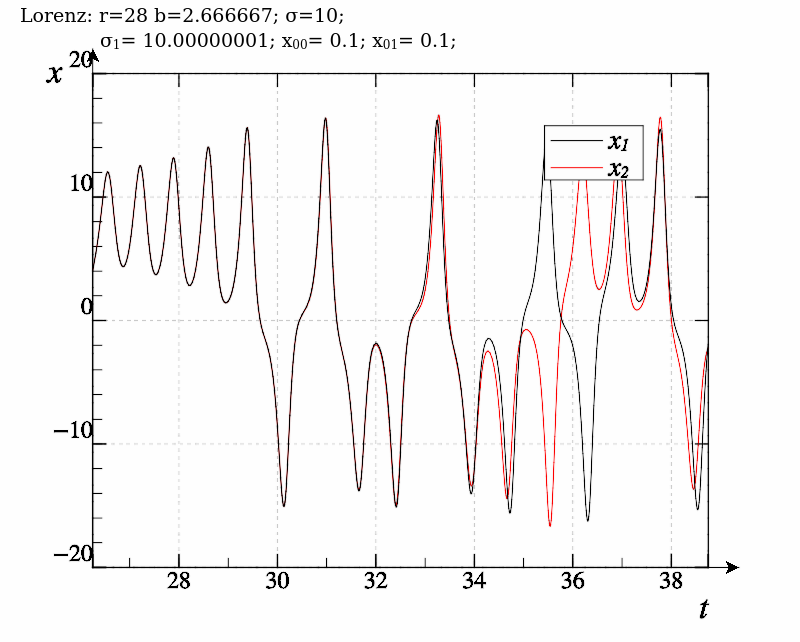
\includegraphics[width=0.49\textwidth]{p/lor_diff-p_xx_sigma.png}
    \hfill
    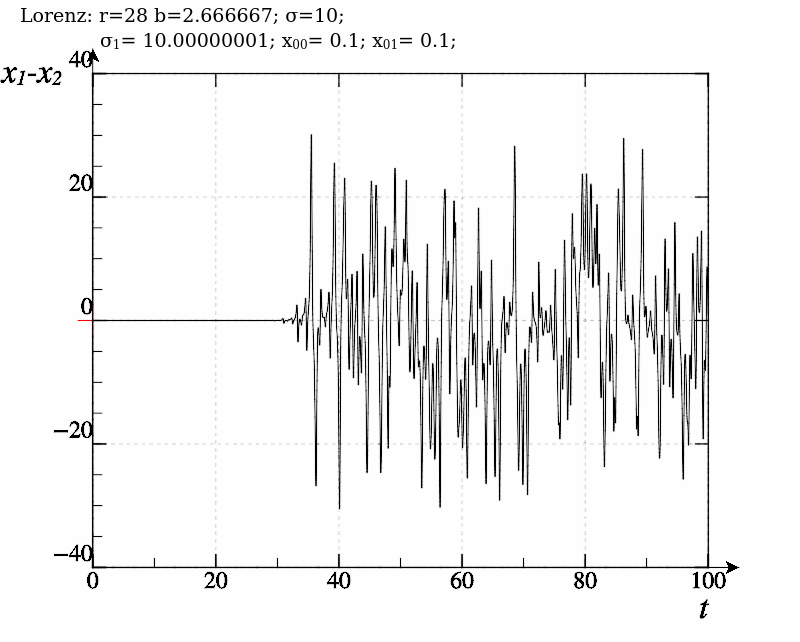
\includegraphics[width=0.49\textwidth]{p/lor_diff-p_dx_sigma.png}
  }
  \caption{Различие в поведение системы Лоренца при малом возмущении параметра $\sigma$}
  \label{atu:f:lor_diff_sigma}
\end{figure}

Эти примеры, демонстрирующие чувствительность фазовых траекторий хаотических систем
как к пренебрежимо малым изменениям параметров, так и к малым изменениям
в состоянии системы, подчёркивают тот факт, что близость
(или даже совпадение, при условии различной истории) параметров модели
и объекта не обозначает близость фазовых траекторий систем
в смысле наиболее часто используемых мер функциональных пространств.
Более того, ввиду плотного заполнения аттракторов таких систем
можно подобрать достаточно близкие траектории для систем с различными значениями параметров
на ограниченном интервале времени.


Следовательно, для синтеза системы идентификации необходимо существование
заданного скалярного критерия $q(x(t))$, близость величин
которых для объекта и модели (в смысле какой-либо меры)
и позволяет говорить о достижении цели идентификации~\cite{crit_method_is}.




Для создания возможности использования критерия
для целей идентификации динамических системы,
сам критерий должен каким-либо образом отображать
глобальные свойства системы, а не её состояния в конкретный момент времени,
то есть не изменяться (по крайней мере существенно),
если свойства системы, предъявляемые в математичкой модели параметрами,
не изменяются. В таких случаях имеет смысл использовать
термин ``интегральные критерии''.



Существует множество способов определения
критериев~\cite{atu_asau11,atu_asau12,atu_asau14,atu_khar_autodor25,atu_asau18,atu_st79,atu_apir2013}.
Для достаточно простых систем вид критерия,
подходящего для задачи идентификации, можно вывести,
определив каким-либо образом исходя из структуры
математической модели.
В некоторых случаях случаях вид критерия можно подобрать эмпирически,
на основании опыта в синтезе систем идентификации для подобных
систем~\cite{atu_asau24}. Тем не менее, наиболее обоснованным
является подход, основанный на использовании
каких-либо физических инвариантов.

Практически в каждом разделе физики существуют
определённые законы сохранения.
Прежде всего стоит назвать общеизвестные и всеобщие
законы сохранения энергии, импульса, момента импульса.
Также существуют и применяются законы сохранения
электрического, лептонного и барионного зарядов,
принцип бесцветности и~т.д~\cite{vigner_invar}.

Наиболее общим, и, следовательно, наиболее употребляемым является
закон сохранения энергии.
Помимо закона сохранения энергии, существуют области,
где имеет смысл применять другие, вплоть до синтетических
законов сохранения, но этот подход
применяется реже.

Каждый из законов сохранения является инвариантом,
и может служить для синтеза критерия в какой-либо области
при определённых условиях.
Тем не менее, непосредственно применение
физических законов сохранения не всегда
удобно и прямолинейно.
Например, в теории управления системы динамического
хаоса относят к ``диссипативным'' системам.
Сам этот термин несколько отличается от аналогичного,
применяемого в физике.
Там система считается диссипативной, если она не
получает энергию извне, а имеющуюся переводит
в не описываемую рассматриваемым комплексом взаимодействий
форму, чаще всего в тепло. \Cmt{ref}
В теории управления
считается, что система, сохраняя процесс диссипации
(перевода энергии в неконтролируемую форму),
получает энергию извне, что и обеспечивает её незатухающую
динамику~\cite{prigogine_selforganization,chernavskii_syn_info,prigogine_order_from_chaos}.
Более того, сам вид уже существующих
математических моделей хаотических систем не позволяет
явно выделить понятие энергии в чистом виде.
В таких случаях
приходится прибегать к полуэмпирическим методам,
рассматривая доступные переменные состояния системы,
проводя анализ их влияния и, в результате моделирования,
выбирая подходящий вид критерия.


Рассмотрим основные способы представления энергии:

Кинетическая энергия тела массой $m$, которое движется со скоростью $v$:
%
\begin{equation}
  E_k = \frac{mv^2}{2} = \frac{m}{2} \left( \od{x}{t} \right)^2.
  \label{atu:eq:Ek_v}
\end{equation}
%
Следует обратить внимание, что, по сравнению с классическим
представлением энергии при обработке сигналов,
здесь присутствует квадратичная зависимость от производной сигнала.

Потенциальная энергия в однородном поле (нулевой уровень выбирается произвольно):
%
\begin{equation}
  E_p = m g x .
  \label{atu:eq:Ep_g}
\end{equation}

Потенциальная энергия в упругом приближении:
%
\begin{equation}
  E_p = k \frac{x^2}{2} .
  \label{atu:eq:Ep_spring}
\end{equation}

Кинетическая энергия вращающегося тела:
%
\begin{equation}
  E_k = J \frac{\omega^2}{2} = \frac{J}{2} \left( \od{\varphi}{t} \right)^2 .
  \label{atu:eq:Ek_spin}
\end{equation}

Внутренняя тепловая энергия:
%
\begin{equation}
  E_t = \frac{im}{2M} RT.
  \label{atu:eq:Et}
\end{equation}

Электрическая энергия, накопленная в конденсаторе:
%
\begin{equation}
  E_c = \frac{C U^2}{2}.
  \label{atu:eq:Ec}
\end{equation}

Энергия магнитного поля, накопленная в катушке индуктивности:
%
\begin{equation}
  E_l = \frac{L I^2}{2} = \frac{L}{2} \left( \od{Q}{t}\right)^2 .
  \label{atu:eq:El}
\end{equation}

Энергия, превращаемая в тепло омическим сопротивлением:
%
\begin{equation}
  E_r = U I = I^2 R = \frac{U^2}{R} = U \od{Q}{t} .
  \label{atu:eq:Er}
\end{equation}



\Cmt{Chemical kinetic -- $\max(x)$}.

\Cmt{Electro-magnetic -- $x\cdot y$}.


Обобщая вышеизложенное, можно сделать вывод, что
несмотря на разнообразие физических процессов, количество способов
представления энергии (рассматриваем сосредоточенные параметры)
весьма ограничено. Основные виды зависимостей:

\begin{itemize}

  \item
    Квадратичная зависимость от координаты: $E \sim x^2$.

  \item
    Линейная зависимость от координаты: $E \sim x$.

  \item
    Квадратичная зависимость от производной координаты по времени: $E \sim \left( \od{x}{t}\right)^2$.

  \item
    Линейная зависимость от произведений координат: $E \sim x \cdot y$.

  \item
    Линейная зависимость от произведений одной координаты на производную другой: $E \sim x \cdot \od{y}{t}$.

  \item
    Максимум величины на заданном интервале времени.

\end{itemize}

Таким образом, в тех случаях, когда нет возможности
использовать явный, непосредственно вытекающий
из строгого анализа системы критерий, в качестве кандидатов
имеет смысл перебрать возможные комбинации из перечисленных выражений.
При этом следует учитывать, что, в отличие от строгих законов сохранения
полученные величины характеризуют систему (или её отдельные элементы)
в достаточно грубом приближении.
Ещё одним важным отличием критериев, построенных по такой схеме,
от строгих законов сохранения является то,
что законы сохранения выполняются строго в каждый момент
(с точностью, обеспечиваемой измерениями). Напротив,
критерии, полученные таким полуэмпирическим путём,
имеют смысл только после какого-либо усреднения.







% Физическая измеримость.

Следствием невозможности непосредственного использования выходных
сигналов объекта и моделей в качестве критерия идентификации, а также
требование физической измеримости критерия является
тот факт, что для получения оценки критерия, как правило,
требуется значительное время~\cite{atu_ich2011,atu_DSMP2016}. % TODO: more ref






% Монотонность -- как следствие одноэкстремальность?


%Зависимость (обозначение?) от времени оценивания.
%Методы измерения.



% }}}2


\subsection{Отличие задачи идентификации от задач решения нелинейного уравнения и поиска экстремума} % {{{2

% \Cmt{Перенести куда-то}

На первый взгляд, при заданном критерии идентификации, задача идентификации
сводится к классической задаче решения нелинейного уравнения: надо найти такие значения
параметров $p$, при которых критерий модели (или какой-либо из моделей)
$q_m$ принимает значение, наиболее близкое к значению критерия объекта $q_o$:
\[
  \mu( q_o, q_m(p) ) \to \min.
\]
Или же при использовании функции качества идентификации $F(q_o, q_m )$ задача
эквивалентна классической задаче поиска экстремума:
\[
  \overline{F}( q_o, q_m(p) ) \to \max.
\]
На самом деле, существуют определённые аспекты, которые делают такое
сведение практически невозможным.

Прежде всего, в задаче в обеих исходных задачах
предполагается, что наблюдаемая система статична:
значение критерия не зависит от времени, и проведя измерение
в точке один раз, можно к нему не возвращаться.
Напротив, идентификация динамической системы предполагает,
что значение критерия, даже после какого-либо усреднения на конечном
интервале времени, есть величина динамическая, причём динамика определяется
не только параметрами системы, но и свойствами самой системы измерения,
а также процессом взаимодействия системы измерения с моделями. При этом
возможны весьма нетривиальные явления, такие как параметрический
резонанс~\cite{landau1}, распространение параметрических волн на множестве моделей и~т.д.

Также существенную роль могут играть как шумы измерения, так и побочные
эффекты от процесса фильтрации шумов.
Применение практически любого фильтра приводит к запаздыванию
в процессе измерения, и игнорирование этих явлений может привести
как к нарушению устойчивости поиска, так и получению совершенно
неадекватных результатов при наличии устойчивости.

В исходных задачах предполагается, что не только
значение функции известно точно в каждой точке, но также известны все производные
(по крайней мере, необходимые для работы метода).
В реальные задачах идентификации производные непосредственно
не доступны для измерения, а их оценка требует применения специальных
методов. При этом процесс оценивания производных, как правило,
более чувствителен к шумам измерения, чем собственно измерение.


% \Cmt{ TODO: Требование конечности производных в условиях дискретного представления сигнала.}

Все эти явления делают задачу идентификации более сложной, чем
исходные задачи, чем и обусловлено
существование широкого спектра методов идентификации. Тем не менее,
некоторые алгоритмы, применимые при поиска экстремума, могут быть
полезны при синтезе системы идентификации.

% Свёртка с чем-то.

Понятие интегрального критерия, применяемого к реальным
задачам, подразумевает не только собственно взятие или оценку интеграла
та выбранном временном интервале, но и нормирование на величину этого интеграла.
Это даёт возможность применяемым критериям не иметь явной мультипликативной
зависимости от времени, и описывать собственно свойства объекта.
Таким образом, интегральный критерий можно представить как
разновидность усреднения для выражения, формирующего данный критерий.
Однако, такие виды усреднения, как среднее арифметическое, медиана и т.д.
неприменимы для формирования критерия для систем с изменяющимся параметром.
Для реализации возможности такого определения необходимо ограничить
по времени усредняемый диапазон.
Оценку этого ограничения обозначим
\label{atu:d:tau_q}$\tau_q$.
В какой-то мере это эквивалентно
применению фильтра нижних частот с частотой среза
\label{atu:d:a_q}$a_q = 1 / \tau_q$.
Рассмотрим возможные реализации такого усреднения.

Самый очевидный способ ограниченного по времени усреднения ---
скользящее среднее~\cite{greshilov_mat_met_prognoz}.
В применяемых терминах, если базовое выражение для формирования критерия
обозначить как $x(t)$, то этот способ усреднения имеет вид:
%
\begin{equation}
  q_{x,a}(t) =
  \frac{1}{\tau_q}
  \int\limits_{t-\tau_q}^{t} x(t) \, dt.
  \label{atu:eq:moving_avarage}
\end{equation}

Суффиксом ``,a'' в определении критерия будем обозначать
именно это определение.
Несмотря на простоту определения, хорошие частотные характеристики,
применения этого метода в реальных задачах довольно неудобно.
Прежде всего, при численной реализации такого интегрирования
необходимо хранить большое количество предыдущих значений,
алгоритмически обеспечить корректный старт при $\tau_q$.
Также при реализации этого метода эффективным алгоритмом,
при котором количество операций на каждом шагу не зависит от $\tau_q$,
возникают вопросы накопления ошибок вычисления.

Менее затратным (с точки зрения объёма вычислений)
является метод экспоненциального сглаживания,
динамику которого применительно к сигналу $x(t)$ можно описать уравнением:
%
\begin{equation}
\od{q_{x,l}}{t}
=
\frac{1}{\tau_q} \left( x(t) - q_{x,l}(t) \right)
\label{atu:eq:qlin}
\end{equation}

Суффикс ``,l'' в дальнейшем изложении будет применяться
для усреднения вида~(\ref{atu:eq:qlin}).
Численная реализация подобного сглаживания не представляет
проблем. Существуют эффективные, в том числе аппаратные
реализации (\ref{atu:eq:qlin}) в дискретном представлении (БИХ-фильтры).
Также возможно, в случае наличия информации о спектральном составе $x(t)$
применении более сложных фильтров для задачи усреднения.
Однако, при идентификации хаотических систем непрерывность спектра
будет препятствовать применению эффективных фильтров.


Если $q(x(t))$  --- подходящий для задачи идентификации критерий,
причём $x(t)>0 \forall t>0$,
$f(x)$ --- строго монотонная функция $\forall x > 0 $,
то и $q(f(x(t))$ --- тоже подходящий для рассматриваемой задачи критерий.
Тем не менее, близость полученной интегральной зависимости в стационарном случае $q(p)$
к линейной позволяет системе идентификации функционировать в близких режимах
на всей области определения~$p$. Для достижения этой цели
при выборе вида критерия следует, если это возможно,
использовать физические соображения для приближения к линейной зависимость $q(p)$,
или же, использовать перебор для выбора наиболее подходящего определения.
С учетом (\ref{atu:eq:Ek_v})--(\ref{atu:eq:Er}) приведём
примеры подобных определений.


\begin{equation}
\od{q_{x^2,l}}{t}
=
\frac{1}{\tau_q} \left( x^2(t) - q_{x^2,t}(t) \right)
,
\label{atu:eq:qx2l}
\end{equation}

\begin{equation}
  q_{xr,a}(t) =
  \sqrt{
    \frac{1}{\tau_q}
    \int\limits_{t-\tau_q}^{t} x^2(t) \, dt
  }.
  \label{atu:eq:qxra}
\end{equation}

\begin{equation}
  q_{|x|,a}(t) =
  \frac{1}{\tau_q}
  \int\limits_{t-\tau_q}^{t} |x|(t) \, dt
  .
  \label{atu:eq:qxma}
\end{equation}

\begin{equation}
  q_{xy^{0.5},a}(t) =
  \sqrt{
    \frac{1}{\tau_q}
    \int\limits_{t-\tau_q}^{t} x(t)y(t) \, dt
  }
  .
  \label{atu:eq:qxy05a}
\end{equation}

При этом следует отметить, что в стационарном случае, при значительных величинах $\tau_q$,
различные методы усреднения дают практически неразличимые результаты, и зависимости
как от $\tau_q$, так и от $t$ становятся пренебрежимо малыми.
Получившуюся зависимость от параметра объекта будем обозначать $q(p)$.


% }}}2

% TODO dynamic q props

% }}}1 _criteria_

\section{Основные понятия и параметры поисковых систем идентификации}  % {{{1

\subsection{Априорная и текущая информация}  % {{{2

Без априорной информации невозможно построение
работоспособной системы идентификации. Основные
априорные величины определяются на этапе постановки
задачи идентификации. В первую очередь это
параметры масштаба: множество допустимых
значений параметров \label{atu:d:p_set}\( \mathcal{P}\),
характерное время работы
идентифицируемой системы~$T$, а также
требуемая точность и скорость идентификации
(могут быть заданы различными способами).
В этот список может входить и ограничения на динамику изменения параметра.
В процессе работы эти параметры могут уточнятся по текущей информации.

Следующую часть априорной (по отношению к идентификации) информации
предоставляет процесс синтеза критерия идентификации.
В первую очередь, это сам вид критерия. Им определятся
как диапазон изменения величины этого критерия $\Delta q$, так и
динамические свойства:
зависимости $\sigma_q(\tau_q)$ или  $\sigma_q(a_q)$,
в простейших случаях, при заданной точности --- характерное/минимально время
оценивания \(\tau_{q,\min}\),
характерное время реакции системы $\tau_p$ на изменение
параметра с учётом динамики измерения \(q\).

Процесс поисковой идентификации заключается в настройке параметров одной
или нескольких моделей, определению критериев идентификации
и соответствующих функций качества, и оцениванию по этой информации
значения идентифицируемого параметра \label{atu:d:p_id}$p_\mathrm{id}$.
При использовании в целях идентификации нескольких моделей,
появляются общие действия, применяемые к каждой из них.

% }}}2


\subsection{Функции качества идентификации и безразмерный вид критерия}  % {{{2


Критерий, основанных на физических принципах --- чаще всего размерная
величина. Даже в тех случаях, когда конкретный вид критерия определён эмпирически
или подбором, критерий чаще всего является размерной величиной.
Как следствие, непосредственное использование величины критерия
достаточно неудобно. Например, при смене единиц измерения,
изменении общего масштаба объекта, значения такого критерия также будут
изменятся, что достаточно неудобно при синтезе системы идентификации.

Вторая проблема вызвана тем, что ни существование достаточно
адекватной модели, ни построение хорошего критерия качества идентификации
не даёт возможность ответить на вопрос о качестве результата,
полученного в процессе работы системы идентификации.
Необходимо внешнее условие, позволяющее оценить полученный результат.
Сравнение в пространстве параметров допустимо практически только для
искусственных модельных задач. Следовательно,
должен быть каким-либо образом задан характерный масштаб
в пространстве критериев, определяющий полученное качество
идентификации.

Есть, как минимум, два подхода к решению данной проблемы.
Первый достаточно очевиден --- все критерии приводятся к безразмерному виду путём деления
на какую-либо характерную величину той же размерности. В качестве такой величины
можно взять максимальное значение критерия при текущих ограничениях,
значение критерия для ``центральной'' точки множества $\mathcal{P}$,
а также подходящую по смыслу и размерности величину, полученную
из анализа физических размерностей.
При этом требуемое качество идентификации задаётся в
выбранных безразмерных единицах.

Второй подход используется при создании экстремальных систем управления
-- введении ``функции качества''.
\Cmt{TODO: ref.}
При использовании введённых обозначений для задачи идентификации
определим её следующим образом:
\label{atu:d:F}$F(q_o, q_m)$.
На эту функцию налагаются следующие требования:

\begin{itemize}

  \item
    Инвариантность к смещению:
    $F(a+c,b+c) = F(a,b)$.
    Невыполнение этого требования обозначает зависимость метода
    от используемой системы координат, и, как следствие --- приводит к логической
    противоречивости метода.
    Если в этом условии положить $c = -b$, то
    очевидно, что для определении функции $F(a,b)$ 
    с двумя аргументами достаточно определить функцию
    с одним аргументом: $ F(a-b,b-b) = F(a-b,0) = F(a-b)$.

  \item
    Симметричность: $ F(a,b) = F(b,a)$ или же $F(a) = F(-a)$,
    что эквивалентно заданию функции как $F(|a|)$.
    Наличие этого требования обусловлено потребностью в получении несмещённых
    оценок идентифицируемого параметра.

  \item
    Существование единственного экстремума с определенным значением, для определённости единичным:
    $F(a,b) = 1  \Leftrightarrow a = b $.
    Ил же в представлении функции с одним аргументом $F(0) = 1$.
    Наличие нескольких экстремумов делает результат процесса идентификации неоднозначным.
    Это требование совершенно не налагает требование одноэкстремальности
    на функцию $F(q(p_m), q(p_o)), \; p_o = \mathrm{const}$. Тем не менее, при
    монотонной зависимости $q(p)$ это будет выполнятся автоматически.

  \item
    Монотонность на каждой из ветвей:
    если $ a_2-b_2 > a_1-b_1, \; a_i-b_i \ge 0$, то $F(a_1,b_1) \ge F(a_2,b_2)$.
    Нарушение этого условия также может привести к нарушению процесса поиска,
    так как при этом вносятся искусственные локальные экстремумы.
    При этом условие $F(a_1,b_1) = F(a_2,b_2)$ допустимо только в удалении от
    рабочей области. Вариант с одним аргументом:
    $ a_2 > a_1, a_1 \ge 0 \to F(a_1) \ge F(a_2)$.

  \item
    Непрерывность --- используется классическое определение из математического анализа.
    Формально это требование не является строго обязательным, многие из рассмотренных
    в работе методов могут сохранить работоспособность и в этом случае. Тем не менее,
    не следует без особой необходимости создавать искусственные помехи нормальному функционированию
    системы идентификации.

\end{itemize}

Эти требования при применении на практике часто дополняются
требованием к простоте реализации функции качества,
или даже к возможности её схемотехнической реализации
без применения элементов вычислительной техники.

Для удобства использования различных функций качества
в одной и той же системе идентификации, а также для
упрощения сравнения свойств исследуемых методов,
примем:
\begin{equation}
  F(a,a) = 1;
  \quad
  \lim\limits_{b \to \pm \infty } F(a,b) = 0.
  \label{atu:eq:F_scale}
\end{equation}




С учётом обозначения
\begin{equation}
  q_r = \frac{q_o - q_m}{q_\gamma},
\label{atu:eq:q_r}
\end{equation}
%
\noindent
отображающего тот факт, что первым этапом построения функции качества
является приведение к безразмерному виду,
представлены наиболее распространённые виды таких функций~\cite{atu_ISDMCI2016,atu_asau24}:
%
\begin{equation}
  F_{\mathrm{gauss}} = \exp( - q_r^2 ),
\label{atu:eq:F_gauss}
\end{equation}
%
\begin{equation}
  F_{\mathrm{parabolic}} = 1 - q_r^2 \left( 1 - \frac{1}{e} \right),
\label{atu:eq:F_parabolic}
\end{equation}
%
\begin{equation}
  F_{\mathrm{triangle}} = 1 - |q_r| \left( 1 - \frac{1}{e} \right),
\label{atu:eq:F_triangle}
\end{equation}
%
\begin{equation}
  F_{\mathrm{hyper}} = \frac{1}{ 1 + |q_r| \left( 1 - \frac{1}{e} \right)},
\label{atu:eq:F_hyper}
\end{equation}
%
\begin{equation}
  F_{\mathrm{log}} = 1 - \ln \left( 1 + |q_r| \right) \frac{1-1/e}{\ln(2)}.
\label{atu:eq:F_log}
\end{equation}

Для всех рассмотренных функций $q_\gamma$ --- величина, обратная чувствительности
функции качества, задаёт масштаб и рабочий диапазон функции качества (рис.~\ref{atu:f:F_types}).
При этом, как правило, значения этих функций могут быть искусственно ограничены диапазоном $[0;1]$.
Каждая из рассматриваемых функций имеет свой набор преимуществ и недостатков~\cite{atu_ISDMCI2016}.
Подробнее этот вопрос будет рассмотрен в главе~\ref{atu:ch:testsys}.

\begin{figure}[htb!]
  \centerline{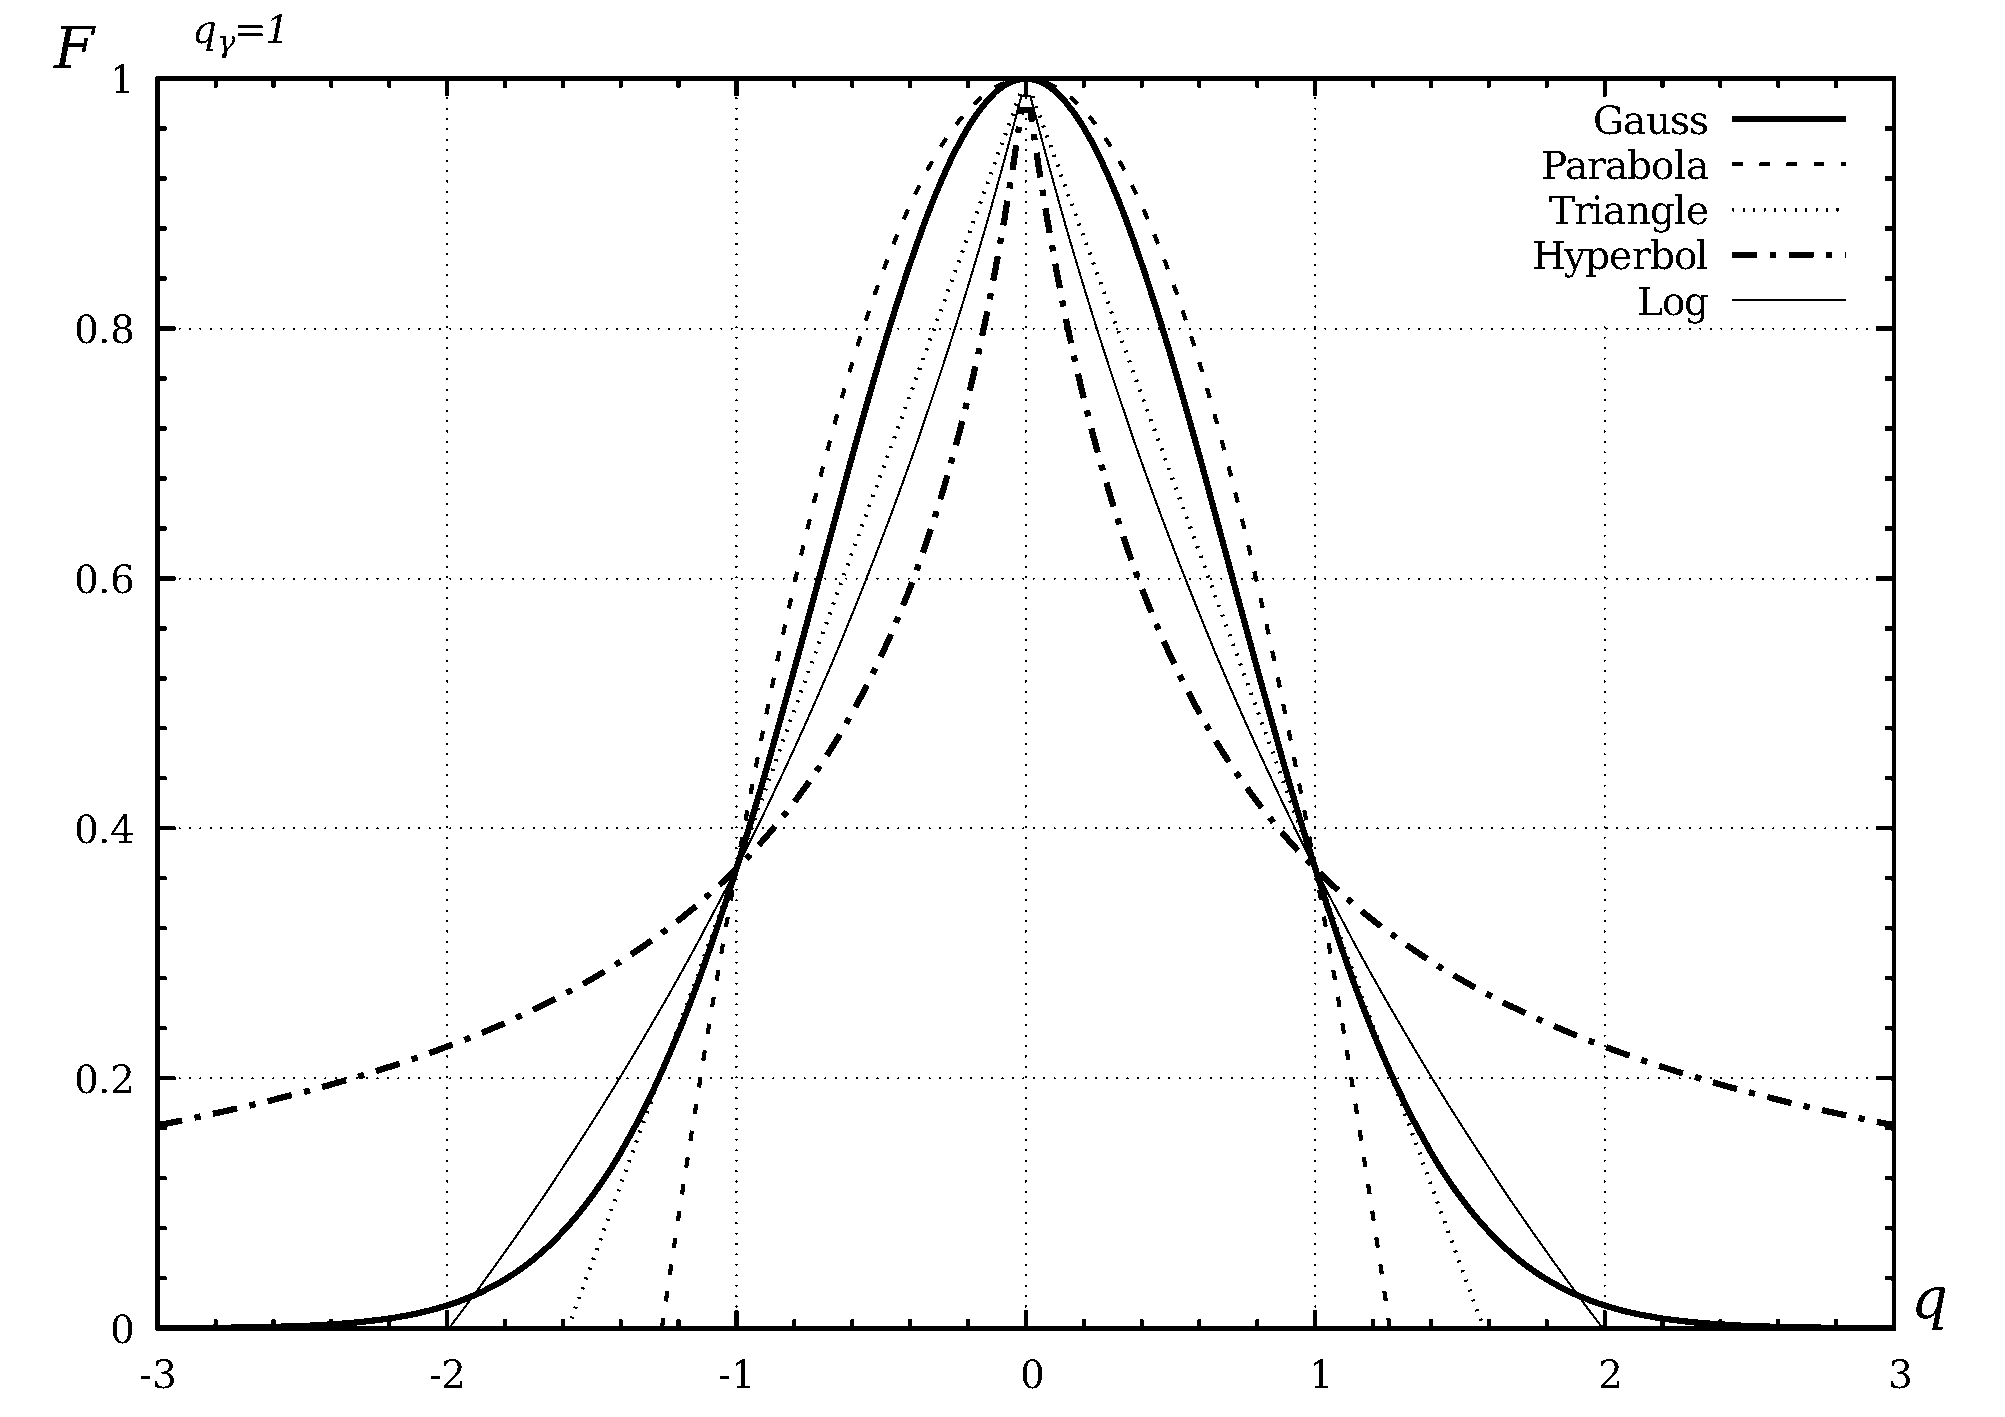
\includegraphics[width=45\TW]{p/F_types.png} }
  \caption{Функции качества идентификации (\ref{atu:eq:F_gauss})--(\ref{atu:eq:F_log})}
  \label{atu:f:F_types}
\end{figure}


% }}}2

% }}}1

\section{Структура поисковых систем}  % {{{1


Введём необходимые для дальнейшего изложения определения.

Определение: \textbf{поисковый агент} --- это динамическая система, получающая выходной ($x(t)$),
и, при необходимости входной сигнал ($u(t)$) от одной или нескольких моделей,
величину критерия идентификации, определённую для объекта $q_o(t)$,
может быть обмениваясь информацией с другими элементами поисковой системы,
на основании значения критерия идентификации
реализующая алгоритм настройки параметра модели (моделей)
таким образом, чтобы обеспечить идентификацию заданного параметра.


Определение: \textbf{координатор поиска} --- это динамическая система, получающая информацию
от поисковых агентов, и на основании этой информации определяющая
$p_\mathrm{id}(t)$ --- искомую величину идентифицируемого параметра.
Помимо этого, координатор может, на основании этой же информации,
управлять процессом адаптации всей поисковой системы.

Таким образом, система идентификации состоит
из множества агентов, и множества координаторов поиска,
совместно решающих задачу идентификации.

За исключением иерархических систем идентификации,
чаще всего используется один координатор поиска.

В простейшем случае, когда используется один поисковый агент,
обязанности агента и координатора могут быть совмещены.
Если отбросить этот вырожденный случай,
наиболее простой является ``плоская'' структура системы идентификации~(рис.~\ref{atu:f:agents_flat}).
При этом координатор единообразно получает информацию от всех поисковых агентов,
и, при необходимости, управляет ими.

\begin{figure}[htb!]
\begin{center}
../../p3/p/agents.pgf
\end{center}
\caption{Мультиагентная система идентификации с плоской структурой}
\label{atu:f:agents_flat}
\end{figure}

В более сложных случаях может использоваться иерархическая структура,
при этом каждый элемент, за исключением первого и последнего
уровня, служит как источником информации для последующего
уровня, так и координатором для предыдущего. При этом элемент
может как иметь непосредственно управляемую модель,
то есть выполнять роль агента, так и довольствоваться ролью промежуточного
координатора.

Некоторые конфигурации агентов и координаторов
в настоящее время практически применяются,
может быть под другими обозначениями и для других задач,
некоторые введены впервые.
Рассмотрим некоторые конфигурации.

\textbf{ Рой } --- множество агентов, обеспечивающее идентификацию за счёт
сосредоточения максимального количества агентов
в области предполагаемого максимума функции качества или же
заданного значения критерия. \Cmt{ref}.
Обычно --- три составляющие поведения
(движение о оцениваемому локальному экстремуму, --- к глобальному, случайная составляющая).

%\Cmt{define}

% \Cmt{Для сравнения требуется и это промоделировать.
% Достаточно накладно --- надо много агентов. Как вариант --- добавить вручную агентов вблизи
% экстремума.}

Достоинством данного подхода является простота алгоритмов,
которые должны быть реализованы агентами.
Недостатки --- требуется избыточное количество агентов.
Значительная часть агентов, находящихся вблизи экстремума,
практически не приносит информации. Роевые
алгоритмы (как и их прообразы в живой природе) ориентированы
для увеличения добычи ресурсов, а не информации. \Cmt{link}.
Также недостатком можно считать необходимость
получения информации от координатора (а именно, значение $p_\mathrm{id}$)
каждым агентом для возможности определения его динамики.

\textbf{ Строй } --- множество агентов, расположение которых,
и если необходимо, смещение, задаётся
единообразным образом.
Отсутствует индивидуальная динамика каждого агента.
Неподвижный строй образует \textbf{сетку},
как равномерно распределённую по пространству параметров,
так и нет.

Сложность алгоритмов, реализуемая каждым агентом в этом случае,
проще, чем в случае роя. Более того, передача информации от
координатора (в данном случае ``командира'') к агенту
является необязательной.
Тем не менее, возможности как адаптации,
так и просто повышения точности идентификации
у данного подхода сильно ограничены.

\textbf{ Ансамбль } --- множество агентов, обеспечивающее идентификацию за счёт
распределения агентов таким образом, который обеспечивает как
точность идентификации за счёт ограниченного скопления агентов
в областях предполагаемых максимумов, так и оперативное переключение
на другие области при изменении параметров за счёт недопущения
неоправданной скученности агентов~\cite{atu_ric2016}.

Возможно применение систем идентификации с структурами и поведением более высокого уровня,
но в данной работе они не рассматриваются.

В данной работе основное внимание уделяется именно
поисковым структурам типа ``ансамбль''.
Очевидным недостатком данного подхода является
относительная сложность алгоритмов, реализуемая поисковыми агентами.


% }}}1

\section{Свойства, параметры и алгоритмы работы поисковых агентов}  % {{{1 -----------

\subsection{Задачи, входные и выходные сигналы поисковых агентов} % {{{2 ------------

В соответствии со своим определением,
один поисковый агент может управлять как одной моделью (рис.~\ref{atu:f:agent1}, \ref{atu:f:agent1q}),
так и несколькими (рис.~\ref{atu:f:agent2}).
При этом он может использовать информацию,
как полученную непосредственно от других агентов,
так и вычисленную в результате обработки данных на других уровнях системы идентификации.

\begin{figure}[htb!]
\begin{center}
% vi:syntax=tex
\begin{tikzpicture}
  \bXStyleBloc{semiboldline,inner sep=2pt};
  \bXLineStyle{medline};
  % --- U
  \bXInput{U};
  % --- M
  \bXBlocL[2.0]{M}{$\mathbf{M}_i$}{U};
  \bXLink[$u(t)$]{U}{M};
  % --- Q
  \bXBloc[3.5]{Q}{$q(t)$}{M};
  \path (Q.east) ++(0.0,-1.0em) coordinate (Qqm);
  \path (Q.south west) ++(-0.3,-0.4) coordinate (BLKlb);
  \bXLink[$x_i(t)$]{M}{Q};
  % --- F
  \bXBloc[2.5]{F}{$F(q_o,q_{mi})$}{Q};
  \path (F.west) ++(0.0,-1.0em) coordinate (Fqm);
  \path (F.west) ++(0.0,+1.0em) coordinate (Fqo);
  \path (Fqo) ++(-1.6em,+2.8em) coordinate (Fqoi) {};  % external input
  \draw[medlinep] (Fqoi) |- (Fqo);
  \node[below right] at (Fqoi) {$q_o(t)$};
  \bXLink[$q_i(t)$]{Qqm}{Fqm};
  % --- P
  \bXBloc[2]{P}{$P$}{F};
  \draw[boldline,<->] (P.north) -- +(0,0.8);
  \path (P.north east) ++(0.1,+0.4) node (BLKrt) {};
  \bXLink[$F_i(t)$]{F}{P};
  % -- output
  \bXOutput[2.8]{Po}{P};
  \bXLink[$p_i(t)$]{P}{Po};
  \bXOutput[1.0]{Por}{P};
  \fill(Por) circle[radius=0.05];
  \bXLineStyle{semiboldline};
  \bXReturn{Por}{M}{$p_i(t)$};
  % -- block
  \draw[subelem] (BLKlb) |- (BLKrt) |- (BLKlb);
  \bXStyleBlocDefault;
  \bXDefaultLineStyle;
  %
  \TikzAddPadding
  %
\end{tikzpicture}

\end{center}
\caption{Поисковый агент, использующий функцию качества $F$, и настраивающий параметр одной модели}
\label{atu:f:agent1}
\end{figure}


\begin{figure}[htb!]
\begin{center}
% vi:syntax=tex
\begin{tikzpicture}
  \bXStyleBloc{semiboldline,inner sep=2pt};
  \bXLineStyle{medline};
  % --- U
  \bXInput{U};
  % --- M
  \bXBlocL[2.0]{M}{$\mathbf{M}_i$}{U};
  \bXLink[$u(t)$]{U}{M};
  % --- Q
  \bXBloc[3.5]{Q}{$q$}{M};
  \path (Q.east) ++(0.0,-1.0em) coordinate (Qqm);
  \path (Q.south west) ++(-0.3,-0.4) coordinate (BLKlb);
  \bXLink[$x_i(t)$]{M}{Q};
  % --- P
  \bXBloc[2]{P}{$P$}{Q};
  \draw[infoline,<->] (P.north) -- +(0,0.8);
  \path (P.west) ++(0.0,-1.0em) coordinate (Pqm);
  \path (P.west) ++(0.0,+1.0em) coordinate (Pqo);
  \path (Pqo) ++(-1.6em,+2.8em) coordinate (Pqoi) {};  % external input
  \path (P.north east) ++(0.1,+0.4) node (BLKrt) {};
  \bXLink[$q_{i}(t)$]{Qqm}{Pqm};
  \draw[medlinep] (Pqoi) |- (Pqo);
  \node[below right] at (Pqoi) {$q_o(t) \qquad A_i$};
  %\bXLink[$F_i(t)$]{F}{P};
  % -- output
  \bXOutput[2.8]{Po}{P};
  \bXLink[$p_i(t)$]{P}{Po};
  \bXOutput[1.0]{Por}{P};
  \fill(Por) circle[radius=0.05];
  \bXLineStyle{semiboldline};
  \bXReturn{Por}{M}{$p_i(t)$};
  % -- block
  \draw[subelem] (BLKlb) |- (BLKrt) |- (BLKlb);
  \bXStyleBlocDefault;
  \bXDefaultLineStyle;
  %
  \TikzAddPadding
  %
\end{tikzpicture}

\end{center}
\caption{Поисковый агент, использующий критерий $q$, и настраивающий параметр одной модели}
\label{atu:f:agent1q}
\end{figure}


\begin{figure}[htb!]
\begin{center}
% vi:syntax=tex
\begin{tikzpicture}
  %\draw[hair,step=1.0em] (0,-3) grid (12.0,3.0);
  \bXStyleBloc{semiboldline,inner sep=2pt};
  \bXLineStyle{medline};
  % --- U
  \bXInput{U};
  \path (U.center) ++(2.5em,0.0em) coordinate (UxM);
  \draw (U.center) -- (UxM);
  \fill (UxM) circle[radius=0.05];
  \node[above right] at(U) {$u(t)$};
  % --- M0
  \bXBranchy[2]{UxM}{U0};
  %\fill[red](U0) circle[radius=0.05];
  \bXBlocL[2.0]{M0}{$\mathbf{M}_{i0}$}{U0};
  \bXLinkyx{UxM}{M0};
  % --- M1
  \bXBranchy[-2]{UxM}{U1};
  %\fill[green](U1) circle[radius=0.05];
  \bXBlocL[2.0]{M1}{$\mathbf{M}_{i1}$}{U1};
  \bXLinkyx{UxM}{M1};
  % --- A
  \path (M0.east) ++(3.1em,0.0em) coordinate (X0);
  \path (X0) ++(4.0em,0.0em) coordinate (P0S);
  \path (X0) ++(0.0em,-2.0em) coordinate (Alb);
  %\fill[red](Alb) circle[radius=0.05];
  \path (M1.east) ++(3.1em,0.0em) coordinate (X1);
  \path (X1) ++(4.0em,0.0em) coordinate (P1S);
  \path (X1) ++(0.0em,2.0em) coordinate (Alt);
  \path ( $0.5*(P0S) + 0.5*(P1S)$ ) coordinate(PS);
  \path ( $0.5*(X0) + 0.5*(X1)$ ) coordinate(QO);
  \draw[medlinep] (QO) ++(-3.2em,0em) -- (QO);
  \node[above left] at(QO) {$q_{o}(t)$};
  %\fill[green](Alt) circle[radius=0.05];
  \draw[boldline] (Alb) -- ++(4.0em,0.0em) |- (Alt) -- cycle; % ----- MAIN block
  \draw[medlinep] (M0.east) -- (X0); // % inputs: x_ix(t)
  \node[above right] at(M0.east) {$x_{i0}(t)$};
  \draw[medlinep] (M1.east) -- (X1);
  \node[above right] at(M1.east) {$x_{i1}(t)$};
  \draw[semiboldlinep] (P0S) -- ++(3.0em,0em) -- ++(0em,-3.0em) -| (M0.south); % -- out params
  \node[above right] at(P0S) {$p_{i0}(t)$};
  \draw[semiboldlinep] (P1S) -- ++(3.0em,0em) -- ++(0em,+3.0em) -| (M1.north);
  \node[above right] at(P1S) {$p_{i1}(t)$};
  \draw[medlinep] (PS) -- ++(4.0em,0em);
  \node[above right] at(PS) {$p_{i}(t)$};
  \path (PS) ++(-2.1em,0.0em) coordinate (AI);
  \node at(AI) {$\mathbf{A}_{i}$};
  %
  \TikzAddPadding
  %
\end{tikzpicture}

\end{center}
\caption{Поисковый агент, настраивающий параметры двух моделей}
\label{atu:f:agent2}
\end{figure}


Для упрощения обозначений величин, относящимся к различным агентам,
ведём обозначения. Если в данном контексте важно указание
индекса агента, то он указывается явно, например:
$F_{c,i}(t)$ --- значение функции качества для центральной (``c'') модели
агента с индексом ``i''. В тех случаях, когда
выбран конкретный агент, или когда обозначение применимо
ко всему множеству агентов, индекс можно упускать, например:
$p_e(t)$\label{atu:d:p_e} --- оценка значения параметра для текущего агента
или же для агентов вообще. Для обозначения ближайшей окрестности
агента используем такие обозначения:
``c'' --- ``center'' --- обозначает центральную или единственную
модель агента, или же относится к агенту в целом,
``l'' --- ``left'' --- обозначает, в зависимости от контекста,
или величину, относящуюся к предыдущему (по индексу) агенту,
или же первую модель (из двух или трёх), используемую
данным агентом,
``r'' --- ``right'' --- аналогично,
но в противоположную сторону в пространстве индексов.
В двумерном случае для второй координаты такую же роль
выполняются обозначения ``t'' --- ``top''
и ``b'' --- ``bottom''.
Если же необходимо указать индекс агента,
а величина относительно объекта
имеет обозначение ``c'', то эту часть обозначения
можно опустить, например:
$ p_i(t) \equiv p_{i,c}(t)$, $q_{i,c} \equiv q_{i}(t)$.
Все индексы одновременно опускать нельзя,
однако, в очевидных случаях можно опускать явную
зависимость от времени:
$ q_l(t) \equiv q_l$.
При необходимости, что величина относится к модели,
без указания конкретного индекса модели,
будем использовать индекс ``m'',
например $x_m$ --- выходной сигнал какой-то
(или же единственной) модели.

В случае, когда один агент настраивает несколько моделей,
или/и, если пространство параметров имеет размерность больше единицы,
вместо простого индекса $i$ могут применяется составные.

Каждый агент на основании как собственных измерений, так и информации,
полученных от других агентов, оценивает значение $p_e(t)$,
которое, по его данным, наиболее близко к $p_o(t)$.
Часть методов использует это представление неявным образом.
При этом, если значение $p_e$ выходит за пределы
значений параметров моделей, на основании которых
было получено это значение, то его следует считать сомнительным.
Степень ``уверенности'' в вычисленном значении $p_e$
обозначим $S \in [0;1]$\label{atu:d:S}(surety).
В результате такие оценки в дальнейшем можно
как вообще исключать из рассмотрения, так и ограничить
его влияние на следующем уровне.
Или, как вариант --- можно ограничить область допустимых
значений $p_e$ значениями параметров используемых моделей.

Выходными сигналами агента являются:\label{atu:d:agent_out_list}

\begin{itemize}

  \item
    $p_c(t)$ -- текущее значение параметра.

  \item
    $p_e(t)$ -- текущее значение оценки параметра.

  \item
    $F_c(t)$ --- текущее значение функции качества
    (если используется одна  модель для агента, или же если агент каким-либо образом её усредняет
    или аппроксимирует в случае нескольких моделей).
    Может совмещать функции входного и выходного сигналов.

  \item
    $q_c(t)$ --- значение критерия качества (аналогично предыдущей величине в случае нескольких моделей);
    изначально этот сигнал был представлен как входной для агента, тем не менее
    он может использоваться и на более высоких уровнях системы идентификации.
    Если же агенту значение критерия недоступно, то и в списке выходных сигналов эта величина
    также отсутствует.

  \item
    $F_e(t)$ --- аппроксимированное значение функции качества
    в точке $p_e(t)$. Если агент не использует для работы аппроксимацию
    $F$, то и выходного сигнала нет.

  \item
    $S(t)$ --- степень ``уверенности'' агента в полученном значении.

\end{itemize}

Некоторые из этих сигналов могут не использоваться в конкретной реализации
координатора поиска. Например, системы идентификации с одним агентом
практически не нуждаются в величине $S(t)$. Величина $q_c(t)$
достаточно редко используется при работе координатора.
Достаточно часто используются производные сигналы,
например $W(t) = F_c(t) S(t)$ (worthiness), совмещающий как локальную
уверенность агента в оценке $p_\mathrm{id}(t)$,
так и глобальную функцию качества.
Также указанные сигналы могут использоваться самим агентом непосредственно,
для определения собственной динамики.


Агенты, для оценивания величины $p_e$
могут использовать как значения критериев идентификации $q$
непосредственно, так и только значения функций качества,
соответствующие критериям.

Принципиальной разницы между конфигурациями
``один агент --- пара моделей''
и
``два агента, каждый управляет одной моделью'' нет.
Для определённости будем считать, что если поддерживается
постоянная разность между значениями параметров моделей,
или же эта разность определяется единообразно,
то это --- один агент. Если же разность
не определяется напрямую, и является следствием динамики каждой модели,
то имеет смысл говорить о паре агентов.

Тем не менее, при использовании пары моделей неоправданно много времени
тратится на перемещение поисковой пары, особенно при резких изменениях
идентифицируемого параметра. Поэтому, использование множества
поисковых агентов может кардинально уменьшить время идентификации.


Рассмотрим случай, когда каждый агент взаимодействует с двумя своими ближайшими соседями.
Для того, что бы обработать границы поисковой области есть несколько подходов,
которые требуют определения дополнительных моделей, использование которых
и обеспечивает как ограничение области поиска, так и единообразность
алгоритмов для агентов внутри.
В дальнейшем будем обозначать их индексами ``ll'' и ``rr''.

Для систем идентификации, использующих только один агент с двумя моделями,
это достаточно неплохой вариант.
Если же использовать несколько агентов, каждый с парой моделей,
то модели в этой системе будут использоваться нерационально.
Рассмотрим случай, когда значения параметров моделей распределены в пространстве
параметров последовательно, и значение параметра, соответствующее $q_o$ лежит между значениями
параметров пары соседних моделей.
При этом, если пара моделей принадлежит одному агенту, то он,
а следовательно, и вся система идентификации может достаточно точно
оценить значение $q_o$. Если же модели этой пары
принадлежат разным агентам --- то нет.

Для того, что бы нивелировать этот недостаток,
попробуем создать систему идентификации,
в которой количество моделей равно количеству агентов,
не считая, может быть, дополнительных моделей на границе рабочей области.

% TODO: really define!!!!!!!!!!!!!


Первый из подходов реализуется наиболее простым способом
и практически не требует затрат.
В этом случае для единообразия множество моделей дополняется двумя
(в одномерном случае) неподвижными псевдомоделями (fake models).
Для псевдомоделей считаем $  F_{ll} = F_{rr} = 0$,
а координаты выбираются за пределами рабочего диапазона поиска.
Применение этого подхода наиболее оправданно для агентов,
вычисляющих значение $p_e$ с помощью функции качества.
При этом, платой за меньшие вычислительные затраты
является появление ``сжимающего'' воздействия на весь ансамбль в целом.
Системы с агентами, которые используют для определения $p_e$ непосредственно значение критерия,
не могут напрямую воспользоваться этом подходом,
так как нулевому (или близкому к нулевому) значению функции качества
обычно соответствует неограниченное множество значений критерия.

Второй подход отличается применением неподвижных настоящих моделей
на границе рабочей области. При этом, агенты, соседствующие с этими моделями,
могут использовать  значения как параметров, так и критериев этих
моделей естественным образом. Основным недостатком этого подхода
является дополнительный расход ресурсов для моделей на границе.
Также применение таких моделей может быть затруднительно тех случаях,
когда моделирование за пределами (или непосредственно на границе)
невозможно из-за нарушения устойчивости моделей.
Тем не менее, этот подход, с одной стороны,
позволяет корректно применять агентов, использующих $q$,
а с другой --- позволяет избавиться от ``сжимающего'' воздействия
при использовании агентов, использующих $F$.

Промежуточным вариантом является подход,
при использовании которого тоже используются
псевдомодели, но вместо нулевого значения
функции качества используется или каким-либо образом аппроксимированное
значение $F$, (применимо и к $q$), или полученное в результате
предварительного моделирования.


% }}}2



\subsection{ Методы определения искомого значения параметра одним агентом }  % {{{2

Первой из задач, стоящих перед агентом идентификации,
является определение $p_e(t)$ на основании
имеющихся данных, а также оценку уверенности $S(t)$
в полученном значении.

Системы поисковой и адаптивно-поисковой идентификации,
используемые для работы с обычными нелинейными динамическими системами,
в качестве исходных данных как для определения непосредственно
искомого параметра, так и для построения поисковой траектории
использовали непосредственно выходные сигналы объекта ($x_o(t)$) и модели~($x_m(t)$).
При этом явно или неявно использовалась функция качества.
Более того, при определённых условиях, с учётом
инерционных и усредняющих свойств системы идентификации
такой подход, неявным образом, использовал
один из энергетических критериев.

При идентификации систем хаотической динамики
использование критерия идентификации является обязательным.
Естественно, это применимо и для систем, не проявляющих
хаотическую динамику. При этом агент,
для выполнения своих задач, может использовать
как как само значение критерия, так и соответствующее ему
значение функции качества. Алгоритмы,
используемые агентами в этих случаях,
будут существенно отличаться. В первую очередь
это связано с тем, что чётный вид функций качества
побуждает использовать для определения максимума
методы, характерный для систем экстремального управления.

Для непротиворечивости и сохранения работоспособности системы идентификации в широких
пределах имеет смысл рассмотреть набор необязательных,
но желательных требований:

\begin{itemize}

  \item
    В первую очередь, при линейной зависимости $q(p)$ и отсутствии ошибок измерения
    ошибка оценивания ``своей'' точки $p_e$ должна быть достаточно малой.
    Нарушение этого требования затрудняет работу системы идентификации
    при приближении к идентифицируемому значению.

  \item
    Во-вторых,
    при этих же условиях глобальные оценки $p_o$ также должны также
    характеризоваться достаточно малыми ошибками, в противном случае
    теряется смысл использования нескольких агентов.

  \item
    Сближение и удаление поисковых агентов в пределах назначенных
    диапазонов не должно приводить к существенному изменению величины
    идентифицируемого значения. Это требование по большей части выполнимо
    только на достаточно ``хороших'' видах критериев, без
    преобладающего влияния высокочастотных нелинейных эффектов,
    однако сам метод не должен вносить существенные дополнительные
    искажения на данном этапе.

\end{itemize}

Следует также отметить, что для реальных задач
$q_o(p) \ne q_m(p)$ ввиду как ограниченности моделей,
так и помех измерения. Тем не менее,
в данной главе данный факт будет игнорироваться
с целью изучения возможностей и ошибок
собственно методов идентификации.




Как уже было отмечено, в задачи агента входит
не только определение величины $p_e$,
но и оценка собственной ``уверенности'' $S$
в полученном значении. Рассмотри факторы,
которые может учитывать агент при решении этой задачи.

\begin{enumerate}

  \item Относительная удалённость точки $p_e$ от точек, использовавшихся при
    её определении. При этом может приниматься во внимание или только центральная точка $p_c$,
    или же учитываться точки соседних агентов.

  \item
    Расположение $p_e$ относительно используемых агентов. Как правило, ошибки при интерполяции
    заметно меньше ошибок при экстраполяции, и это необходимо учитывать. Также,
    сама конфигурация используемых точек может быть более или менее благоприятна
    для оценки~$p_e$.

  \item
    В при использовании некоторых методов есть возможность оценить нелинейность
    зависимости $q(p)$, и следовательно, учесть это при определении $S$,
    с помощью коэффициента~$k_l$.

  \item
    При оценке могут возникать особые случаи, препятствующие
    нормальной работе метода. Следовательно, такие случаи требуют применения особых правил
    при вычислении~$S$.

\end{enumerate}

В учётом вышеизложенного, предлагаются
следующие способы определения $S$:
%
\begin{equation}
  S_1 = c_\mathrm{su} \exp \left( - \frac{ \big( k_l c_\mathrm{dist} ( p_e - p_c ) \big)^2 }{p_b^2} \right)
  ,
  \label{atu:eq:S1}
\end{equation}
%
\begin{equation}
  S_3 = c_\mathrm{su} \exp \left( - \frac{ \big( k_l c_\mathrm{dist} \min( |p_e - p_l|,|p_e - p_c|, |p_e - p_r| ) \big)^2 }{p_b^2} \right)
  .
  \label{atu:eq:S3}
\end{equation}
%
где
$c_\mathrm{su}$ --- коэффициент, отражающий работоспособность метода в рассматриваемом случае;
$c_\mathrm{dist}$ ---  коэффициент, определяющий ``штраф'' или ``бонус'', связанный с относительным расположением рабочих точек;
$k_l$ --- коэффициент оценки нелинейности системы;
$p_b$ --- характерный масштаб, относительно которого учитывается удаление $p_e$ от используемых точек.

В случаях, когда агенты равноправны, имеет смысл использовать определение (\ref{atu:eq:S3}),
так как ошибка определения $p_e$ в первую очередь определяется
её удалённостью от ближайшего агента, в данной работе, если не указано обратное,
будет использоваться именно оно. Использовать определение (\ref{atu:eq:S1}) имеет смысл в тех случаях,
когда информация, полученная от соседних агентов, менее надёжна, чем от текущего,
например, при использовании псевдомоделей.




\paragraph{Демонстрационная задача}

Для демонстрации способов определения поисковым агентом
величины $p_e$ в стационарном или квазистационарном случае
введём следующую искусственную зависимость $q(p)$:
%
\begin{equation}
  q_\mathrm{dem}(p) = q_{00} + c_\mathrm{lin} \tilde{p} + c_\mathrm{s1} \sin( \pi \tilde{p} ) + c_\mathrm{s2} \sin( 2 \pi \tilde{p} ) + c_\mathrm{s20} \sin( 20 \pi \tilde{p} ),
  \label{atu:eq:q_dem}
\end{equation}
%
где $q_{00}$, $c_\mathrm{lin}$, $c_\mathrm{s1}$, $c_\mathrm{s2}$, $c_\mathrm{s20}$
--- коэффициенты, позволяющие
настроить эту зависимость для проверки заданного аспекта поведения агента,
$ \tilde{p} = \frac{p - p_{\min}}{p_{\max} - p_{\min}} $ --- параметр, приведённый к безразмерному виду.
При этом $\tilde{p} \in[0;1]$, $c_\mathrm{lin} \ne 0$ определяет линейную часть зависимости,
$c_\mathrm{s1}$ и $c_\mathrm{s2}$ определяют нелинейную часть, имеющую характерный масштаб
порядка рабочего диапазона $p$,
а $c_\mathrm{s20}$ определяет высокочастотную составляющую этой зависимости.
Если $c_\mathrm{s1} = 0$, $c_\mathrm{s2}=0$, $c_\mathrm{s20}=0$,
то задача определения $p_e$ становится тривиальной,
но такой случай также является полезным для анализе поведения агента.

В дальнейшем будем использовать эти обозначения при описании
различных режимов работы методов идентификации, а также
при моделировании тестовых задач.

Рассмотрим возможные способы определения $p_e$ для агентов,
использующих как критерий идентификации непосредственно,
так и функции качества.

% }}}2


\subsection{Методы агентов, использующих значения критерия }  % {{{2

Неподвижный агент, использующий для своей работы только одну модель,
и, соответственно, характерное для неё значения критерия,
практически не имеет самостоятельного смысла. Реальная польза от такого агента
может быть только в том случае, когда координатор
каким-то образом смог оценить зависимость $q(p)$ целиком,
и передал или эту зависимость агенту, или по его запросу вычисляет $p(q)$.
Очевидно, что в таком случае никакие поисковые агенты не нужны,
и можно просто вычислить $p(q_o)$.

Если агент, использующий одну модель является подвижным,
то он может оценить своё положение, используя историю.
Представление истории может иметь различные формы.
Например, агент может хранить значения $p_c$, $q_c$
для момента времени в прошлом, отстоящем от текущего
на заданное значение. Может быть применён какой-либо
сглаживающий фильтр, в котором влияние различных моментов прошлого учитывается
с различными коэффициентами. Также в качестве функции
представления истории может использоваться
динамика самого идентифицируемого объекта~\cite{mich_92}.

Рассмотрим случай, когда один подвижный агент и получает данные с двух моделей,
$ \mathbf{M}_{il}$ и
$ \mathbf{M}_{ir}$,
и управляет ими единообразным образом, например
выдерживая постоянное расстояние $\Delta p$ между ними в пространстве параметров.
В этом случае он может оценить, какая из моделей ближе по критерию
к объекту, и оценить положение $p_o$ как $p_e$.

Рассмотрим группу из трёх агентов:
$\mathrm{A}_l$,
$\mathrm{A}_c$,
$\mathrm{A}_r$.
Агент $\mathrm{A}_c$ со значением параметра $p_c$
сам определяет величину $q_c$,
от соседних агентов получает значения
$p_l$, $q_l$, $p_r$, $q_r$.
Будем считать, что динамика агентов определена так,
что $p_l(t) < p_c(t) < p_r(t) \; \forall t$.
Система идентификации обеспечивает каждого
агента значением $q_o$. С учётом всего вышеперечисленного,
задача определения $p_e$ заключается в нахождении такого $p$,
которое соответствует пересечению неизвестной кривой,
заданной тремя точками, с прямой $q=q_o$.
Формально, с учётом введённых ограничений,
три точки однозначно определяют параболу.
Однако, применение параболической аппроксимации в условиях
высокого уровня помех чаще всего неоправданно~\cite{atu_asau27}. Более того,
в этом случае потребуется дополнительная логика как для
выбора подходящего корня, так и для определения
``уверенности'' в полученном решении. Поэтому, будем рассматривать
кусочно-линейное приближение с анализом полученной конфигурации.

Рассмотри возможные конфигурации в порядке,
обеспечивающем непротиворечивость алгоритма.

\paragraph{Случай 1.}
Это особый случай, когда значение $p_c$ агента
достаточно хорошо совпадает с искомым значением.
Понятие ``достаточно хорошо'' в данном случае определяется
поставкой задачи, и может быть задана предельным значением
функции качества: $F_c > F_{\mathrm{good}}$, где $F_{\mathrm{good}}$
выбирается достаточно близко к единице.
При этом считаем:
%
\[
p_e = p_c, \; c_\mathrm{su} = 1, \;  c_\mathrm{dist} = 1, \;  k_l = 1, \;  p_b = p_r - p_l,
\]
%
что даёт $S = 1$, т.е. агент полностью ``уверен''
в полученном значении $p_e$. Если есть явное ограничение
на использование функции качества непосредственно агентом,
то следует задать допуск на значение критерия:
$ |q_c-q_o| < q_{\min}$.

Практически, для нескольких агентов может одновременно
может выполнится данное условие, и
дальнейшее определение $p_\mathrm{id}$ в этом противоречивом случае
возлагается на координатора поиска. Если данная
ситуация в процессе поиска случается достаточно редко,
то это, как правило, не нарушает общую динамику поиска.
Если же этот случай проявляется достаточно часто,
то это свидетельствует о грубых просчётах
при синтезе системы идентификации.
Например, такое поведение может вызвать применение
критерия, неподходящего для данной задачи,
или же предельно заниженная чувствительность функции качества.

Следует отметить, что в этом случае у агента нет необходимости
анализировать значения, полученные от соседних агентов.
Это позволяет избежать ряда ситуаций, в которых
алгоритм поиска будет давать сбои, связанные неопределённостью
алгоритмов поиска в вырожденных случаях.
В первую очередь,
если $F_c \le F_\mathrm{good}$, то $q_o -q_c \ne 0$,
и можно применить следующие преобразования:
%
\[
  \tilde{p}_l = p_l - p_c;
  \quad
  \tilde{p}_c = p_c - p_c = 0;
  \quad
  \tilde{p}_r = p_r - p_c;
  \quad
  \tilde{p}_e = p_e - p_c;
\]
\begin{equation}
  \tilde{q}_l = \frac{q_l-q_c}{q_c-q_o};
  \quad
  \tilde{q}_c = \frac{q_c-q_o}{q_c-q_o} = 1;
  \quad
  \tilde{q}_l = \frac{q_l-q_c}{q_c-q_o}.
  \label{atu:eq:q_agent_rel}
\end{equation}
%
При этом критерий приводится к безразмерному виду,
причём точку отсчёта и единичную длину определяют величины
$q_c$ и $q_o$, так как $\tilde{q_c} = 1$ и $\tilde{q_o} = 0$.
В пространстве параметров происходит только смещение точки отсчёта.

С учётом этих обозначений определим оценку $\tilde{p}_e$
для каждого из участков независимо:
%
\begin{equation}
  \tilde{p}_{el} = \frac{\tilde{p}_l}{1-\tilde{q}_l},
  \quad
  \tilde{p}_{er} = \frac{\tilde{p}_r}{1-\tilde{q}_r}.
  \label{atu:eq:pr_ex}
\end{equation}

Случай точного равенства нулю знаменателя в этих выражениях соответствует
бесконечно далёкому расположению $p_e$, полной неуверенности в полученном решении
($S = 0$) и алгоритмически исключается.


\paragraph{Случай 2.} % brIdx = 3,4,5,6
Все значения $q_l$, $q_c$, $q_r$ лежат по одну сторону
сторону от прямой $q=q_o$,
что эквивалентно условию $\tilde{q}_l > 0  $ и $\tilde{q}_r > 0  $.
В этом случае следует принять,
что $p_e \notin [p_l, p_r]$, то есть по данным текущих трёх моделей
нет возможности достаточно уверенно определить $p_e$. Тем не менее,
задача оценить $p_e$ всё равно остаётся актуальной.
Если система идентификации использует только одного агента,
то значение $p_e$, пусть даже ненадёжное, необходимо для
определения динамики агента, и соответственно, смещении
его в сторону области, где оценка будет более обоснованной.
Если же используется мультиагентная система,
то полученное значение $p_e$ достаточно или ограничить искусственно,
или уменьшить его значимость за счёт снижения величины $c_\mathrm{su}$.

При анализе данного случая необходимо рассмотреть несколько
вариантов.

Вариант A.\label{atu:d:p_eql_2A} % brIdx = 3
Центральная точка --- наилучшая~(рис.~\ref{atu:f:pq_2A}),
т.е $\tilde{q}_l > 1 $ и $\tilde{q}_r > 1  $.

\begin{figure}[htb!]
  \centerline{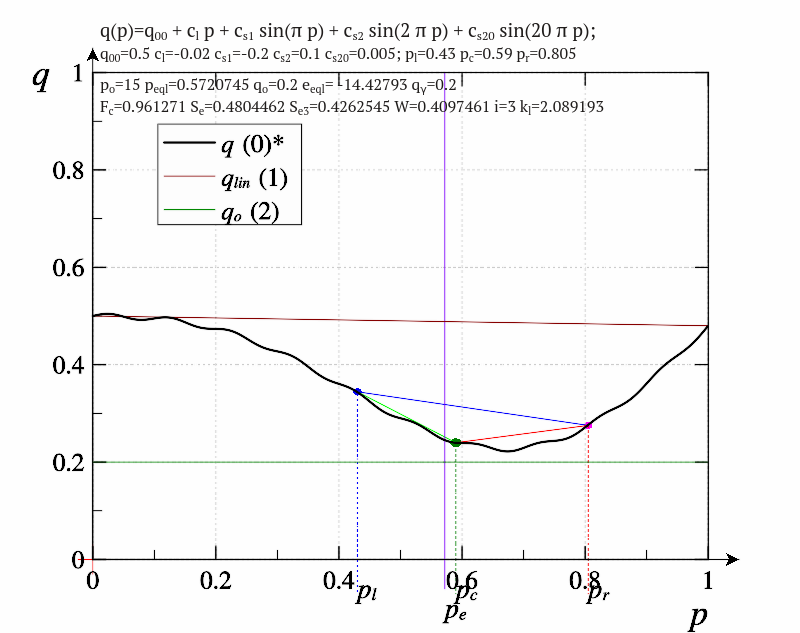
\includegraphics[width=60\TW]{p/pq_sin-p_pq_cgood.png} }
  \caption{Конфигурация точек, соответствующая случаю 2A}
  \label{atu:f:pq_2A}
\end{figure}

Как видно из графика, это достаточно нетривиальная конфигурация,
которая может соответствовать локальному приближению
$q(p)$ к $p_o$, что для хорошего критерия нехарактерно,
временной конфигурации рабочих точек из-за влияния помех,
а также возможности реального нахождения $p_o$
в текущем рабочем диапазоне, но из-за определённых причин,
прежде всего сильной нелинейности $p(q)$
неправильной оценке его положения.
На основании имеющейся информации сложно сделать вывод
о реальных причинах, поэтому
в этом случае производится минимальная корректировка положения,
и уверенность в полученном решении невелика:
%
\begin{equation}
  \tilde{p}_e = 0.1 ( \tilde{p}_{el} + \tilde{p}_{er} ),
  \;
  c_\mathrm{su} = 0.2, \;  c_\mathrm{dist} = 4, \;   p_b = p_r - p_l,
  \label{atu:eq:pr_e_2A}
\end{equation}



Вариант B.\label{atu:d:p_eql_2B} % brIdx = 4,5
Центральная точка --- промежуточная~(рис.~\ref{atu:f:pq_2B}).
Соответствует условию
$ ( \tilde{q}_l -1 ) \cdot ( \tilde{q}_r -1 ) < 0 $.

\begin{figure}[htb!]
  \centerline{
    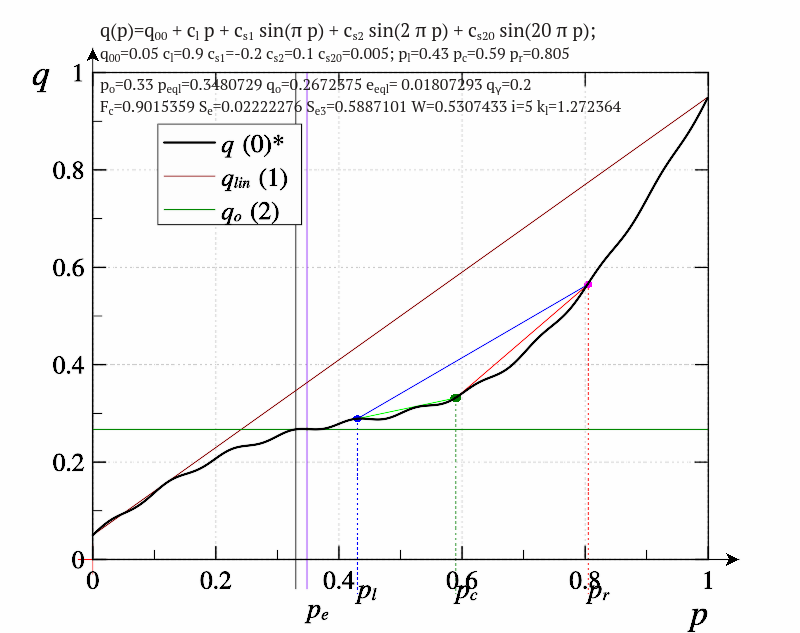
\includegraphics[width=49\TW]{p/pq_sin-p_pq_po=033.png}
    \hfill
    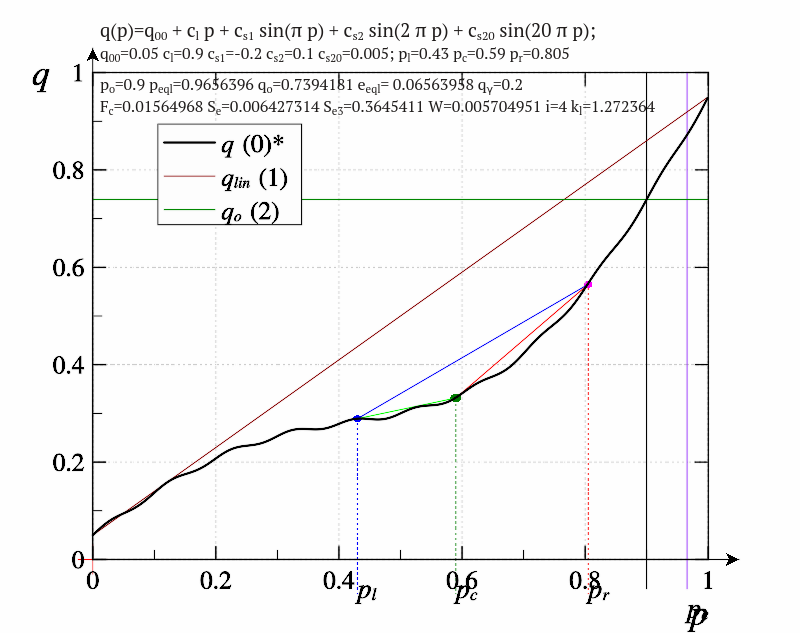
\includegraphics[width=49\TW]{p/pq_sin-p_pq_po=090.png}
  }
  \caption{Конфигурации точек, соответствующие случаю 2B}
  \label{atu:f:pq_2B}
\end{figure}

Эта конфигурация не является неопределённой, как в предыдущем случае,
и соответствует экстраполяции зависимости за пределы $[p_l, p_r]$.
В этом случае будем использовать
%
\begin{equation}
  \tilde{p}_e
  =
  \begin{cases}
    \tilde{p}_{el}, & \tilde{q}_l < \tilde{q}_r
    \\
    \tilde{p}_{er}, & \text{ otherwise}.
  \end{cases}
  ,
  c_\mathrm{su} = 0.9, \;  c_\mathrm{dist} = 2,  \;
  p_b =
  \begin{cases}
    -\tilde{p}_l, & \tilde{q}_l < \tilde{q}_r
    \\
    \tilde{p}_r, & \text{ otherwise}.
  \end{cases}.
  \label{atu:eq:pr_e2B}
\end{equation}

Относительно высокое значение
$ c_\mathrm{su}$ и достаточно ограниченное значение $c_\mathrm{dist}$
подчёркивают тот факт, что несмотря на наличие экстраполяции,
метод в этом случае может давать неплохие результаты.


Вариант C. \label{atu:d:p_eql_2C}% brIdx = 6
Центральная точка --- наихудшая~(рис.~\ref{atu:f:pq_2C}).

\begin{figure}[htb!]
  \centerline{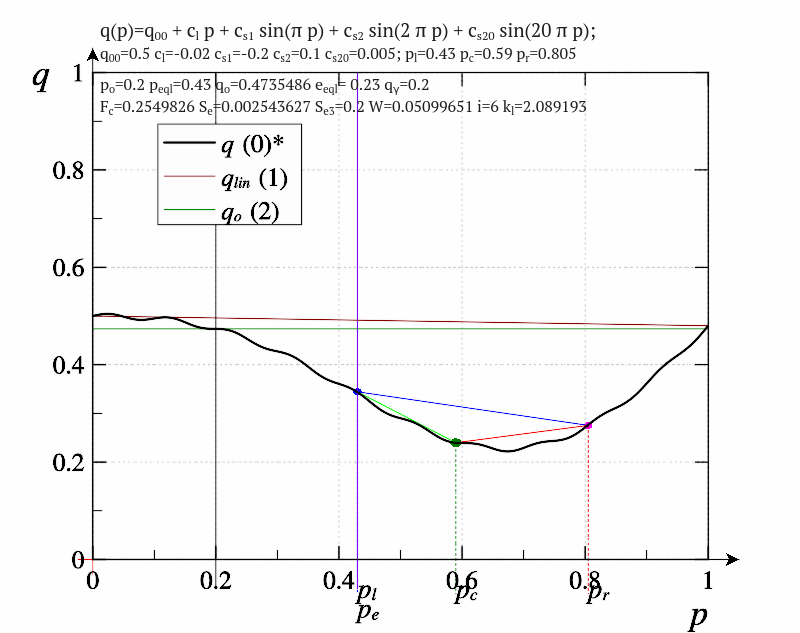
\includegraphics[width=60\TW]{p/pq_sin-p_pq_cbad.png} }
  \caption{Конфигурация точек, соответствующая случаю 2C}
  \label{atu:f:pq_2C}
\end{figure}

Этот вариант один из наименее благоприятных для определения $p_e$,
ещё более неопределённый по сравнению со случаем 2A.
В этом случае в качестве $p_e$ можно взять лучшую из крайних точек,
при этом нулевое расстояние от этой точки в определении $S$
необходимо скомпенсировать существенным штрафом в значении $c_\mathrm{su}$,
остальные коэффициенты при этом значения не имеют:
%
\begin{equation}
  \tilde{p}_e
  =
  \begin{cases}
    \tilde{p}_{l}, & \tilde{q}_l < \tilde{q}_r
    \\
    \tilde{p}_{r}, & \text{ otherwise}.
  \end{cases}
  ,
  c_\mathrm{su} = 0.1 .
  \label{atu:eq:pr_e2C}
\end{equation}

\paragraph{Случай 3.} % brIdx = 10
Значения $q_l$ и $q_r$ лежат по одну сторону от прямой $q=q_o$,
а $q_c$ --- по другую, то есть существуют два корня в рассматриваемой области~(рис.~\ref{atu:f:pq_3}).

\begin{figure}[htb!]
  \centerline{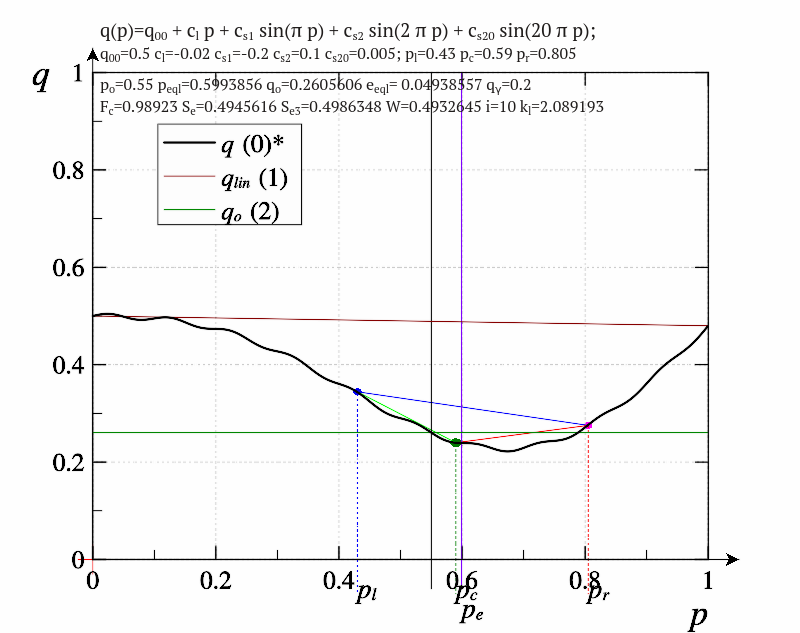
\includegraphics[width=60\TW]{p/pq_sin-p_pq_double.png} }
  \caption{Конфигурация точек, соответствующая случаю 3}
  \label{atu:f:pq_3}
\end{figure}

Это достаточно нетривиальный случай,
и при правильном критерии и идеальных условиях
встречаться не должен. Однако, в реальных условиях,
при наличии ошибок изменения и несовершенстве критерия
данный случай вполне возможен (пусть и достаточно редко), и требует отдельной обработки.
Более того, в отличие от неопределённых случаев 2A и 2C,
данный свидетельствует о том, что искомое значение
действительно лежит в текущем рабочем диапазоне,
но помехи и нелинейности не дают возможности установить его
точное положение. При этом, если для определения $p_e$
выбрать один из интервалов $[p_l,p_c]$ и $[p_c, p_r]$,
то этот выбор, с учётом помех, будет практически случайным,
и малые изменения в значениях критерия могут переключить на другую ветвь.
Поэтому, для определения $p_e$ используем подход, аналогичный применённому
в случае 2A, но с другими коэффициентами:
%
\begin{equation}
  \tilde{p}_e = 0.1 ( \tilde{p}_{el} + \tilde{p}_{er} ),
  \;
  c_\mathrm{su} = 0.5, \;  c_\mathrm{dist} = 2, \;   p_b = \frac{p_r - p_l}{2}.
  \label{atu:eq:pr_e_3}
\end{equation}


\paragraph{Случай 4.}
Две последовательные точки лежат по одну сторону от прямой $q=q_o$,
а оставшаяся --- по другую, то есть в рабочем диапазоне
существует только одно пересечение~(рис.~\ref{atu:f:pq_4}).


\begin{figure}[htb!]
  \centerline{
    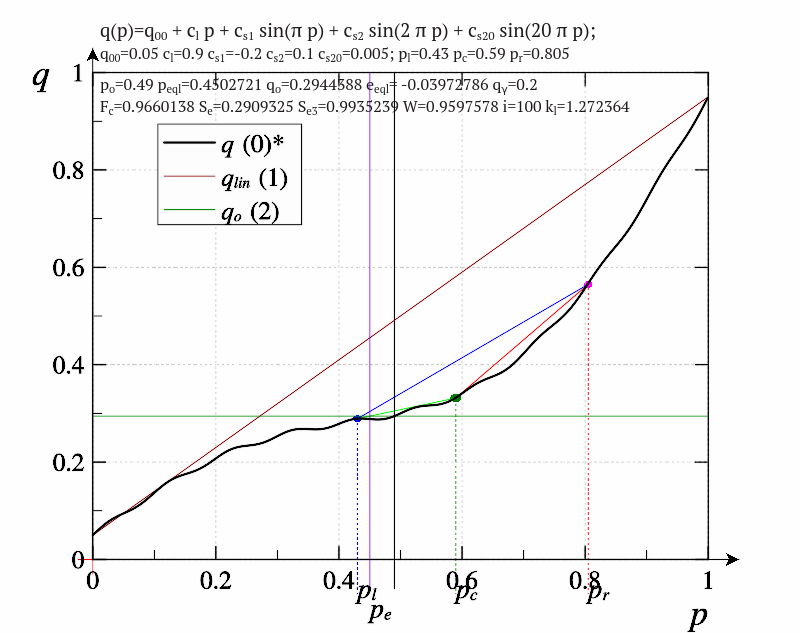
\includegraphics[width=49\TW]{p/pq_sin-p_pq_po=049.png}
    \hfill
    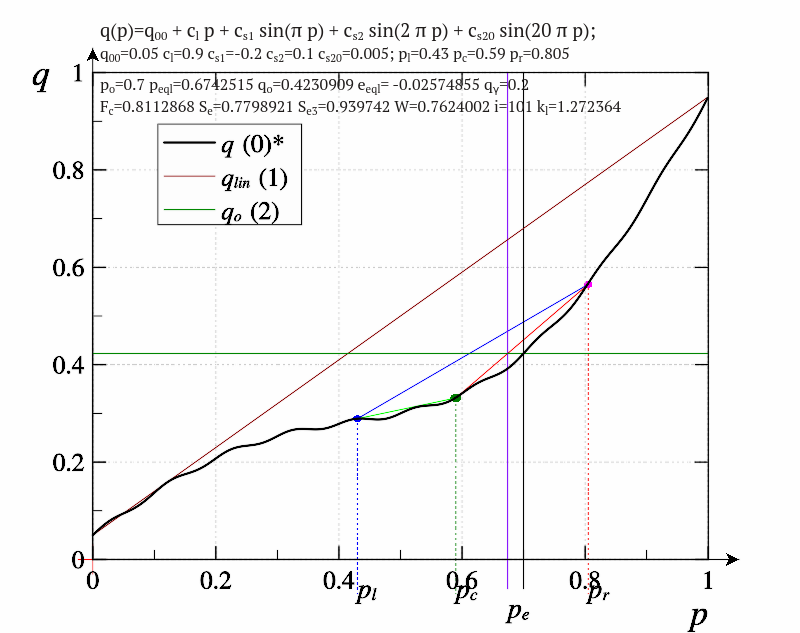
\includegraphics[width=49\TW]{p/pq_sin-p_pq_po=070.png}
  }
  \caption{Конфигурации точек, соответствующие случаю 4}
  \label{atu:f:pq_4}
\end{figure}

В этом, самом благоприятном случае
производится интерполяция,
а не экстраполяция зависимости $q(p)$,
и достаточно выбрать тот участок, на котором
гарантированно происходит пересечение.
При этом значения всех коэффициенты подчёркивают
уверенность агента в определённом значении $p_e$:
%
\begin{equation}
  \tilde{p}_e
  =
  \begin{cases}
    \tilde{p}_{el}, & \tilde{q}_l < 0
    \\
    \tilde{p}_{er}, & \text{ otherwise}.
  \end{cases}
  ,
  c_\mathrm{su} = 1.0, \;  c_\mathrm{dist} = 0.5,  \;
  p_b =
  \begin{cases}
    -\tilde{p}_l, & \tilde{q}_l < 0
    \\
    \tilde{p}_r, & \text{ otherwise}.
  \end{cases}.
  \label{atu:eq:pr_e4}
\end{equation}

В любом из рассмотренных случаев, имеет смысл ввести дополнительное ограничение
на значение $p_e$, так как из-за ошибок измерения и моделирования
оно может оказаться даже вне диапазона $[p_{\min}, p_{\max}]$.
С практической точки зрения достаточно хорошо зарекомендовало себя ограничение
$ \tilde{p}_r \in [2\tilde{p}_l, 2\tilde{p}_r ]$.
С учётом низкого значения $S$ для агентов, попавшим под такое ограничение,
их влияние на общий результат будет минимальным,
так как нормальном течении процесса идентификации существует
хотя бы один агент с высоким значением $S$.
Более строгие ограничения достаточно редко оправдывают себя,
так как при этом не используются экстраполяционные свойства агентов.

Описанный данными правилами способ
определения
$p_e$ в дальнейшем изложении будем обозначать $p_{eql}$\label{atu:d:p_eql}.

\paragraph{Учёт влияния оценки линейности зависимости $q(p)$}

В предшествующих рассуждениях при вычислении коэффициента ``уверенности'' $S$
в расчёт принималось только расстояние от текущих значений параметров модели для $p_e$.
При этом не учитывалась возможность оценки линейности аппроксимации $q(p)$
по имеющимся данным. При этом оценка должна быть независима от изменения масштаба
как параметров, так и критериев, иметь удобную форму для дальнейшего
использования, и не требовать вычислений, сильно чувствительным к помехам измерений.

Так как в рассматриваемом случае один агент наблюдает значения $p$ и $q$
для трёх моделей, то оценить влияние нелинейных факторов он может
следующим образом. В первую очередь, по значениям, соответствующим крайним точкам
линейной интерполяцией оценивается значение $q_c$ (или же после нормализации --- $\tilde{q}_c$):
%
\begin{equation}
 q_{c,\mathrm{lin}}
  =
  \frac{  q_l \left( p_r - p_c \right) + q_r \left( p_c - p_l \right) }{p_r-p_l},
  \label{atu:eq:q_clin}
\end{equation}
%
\begin{equation}
  \tilde{q}_{c,\mathrm{lin}}
  =
  \frac{ \tilde{q}_l \tilde{p}_r - \tilde{q}_r \tilde{p}_l }{\tilde{p}_r-\tilde{p}_l}  .
  \label{atu:eq:qr_clin}
\end{equation}

Для обеспечения корректности и малой чувствительности полученных оценок
к ошибкам измерения следует обеспечить достаточное расстояние между соседними агентами.
Это требование необходимо учитывать при определении динамики агентов.
С другой стороны, проведении всех предыдущих оценках величины $p_e$
неявно предполагалось $\tilde{p}_l < 0$ и $\tilde{p}_r > 0$.
Следовательно, на начальном этапе работы метода случай чрезмерной близости агентов
детектироваться автоматически и обрабатываться отдельно особым образом.
Например, в этом случае имеет смысл принять $p_e = p_c$
при сохранении достаточно высоких значений $S$ --- если метод привёл
несколько агентов в малую окрестность одной точки, то
или точка действительно близка к искомой, или же весь метод
недостаточно пригоден для решения поставленной задачи.


Из полученных оценок $q_{c,\mathrm{lin}}$, $\tilde{q}_{c,\mathrm{lin}}$
сформируем следующие безразмерные коэффициенты, позволяющие оценить
нелинейность $q(p)$:
%
\begin{equation}
  k_l = 1 + \frac{|q_c - q_{c,\mathrm{lin}}|}{|q_r-q_l|} ,
  \label{atu:eq:k_l1}
\end{equation}
%
\begin{equation}
  k_l = 1 + \frac{|\tilde{q}_c - \tilde{q}_{c,\mathrm{lin}}|}{ |\tilde{q}_r-\tilde{q}_l|} .
  \label{atu:eq:k_l2}
\end{equation}

Данное представление $k_l$ было выбрано с целью непосредственного использования
этой величины в $S$, т.е. если $\tilde{q}_{c,\mathrm{lin}} \to \tilde{q}_c$,
то $k_l \to 1$, и есть основания полагать, что на расстояниях порядка $p_r-p_l$
оценка $p_e$ достаточно состоятельна. С другой стороны,
если $k_l \gg 1 $, то нелинейные эффекты в рассматриваемой области
преобладают над линейными, и оценку $p_e$  стоит рассматривать как недостоверную.
При практическом использовании имеет смысл искусственно ограничить эту величину,
например $k_l < 100 $, так как неограниченный рост при стремлении знаменателя
к нулю принципиально ничего не меняет в работе метода, но при этом
возможны проблемы чисто вычислительного характера.





% }}}2

\subsection{Методы агентов, использующих значения функции качества }  % {{{2

Единственный неподвижный агент,
использующий значение функции качества,
ещё более бесполезен (с точки зрения синтеза системы идентификации),
чем один неподвижный агент,
использующий значение критерия, так как в этом случае даже наличие
зависимости $q(p)$ не даёт возможности однозначно определить
значение параметра.
Он может сигнализировать о том, что в пределах
\(\tau\) модель была или не была достаточно адекватна
объекту.




Наличие истории и возможность перемещаться дают возможность
построить систему идентификации и на одном агенте.
В качестве истории могут использоваться, в том числе,
динамические свойства идентифицируемого объекта
(оригинальный метод АПИ). Также могут быть
применены интегрирующие элементы агента идентификации
(синхронный детектор, \ldots).

В простейших случаях возможно построение системы идентификации
с одной моделью и, соответственно, одним поисковым агентом.
Примерами такого похода могут служить
метод синхронного детектора \cite{adopt_cont_sys}
и оригинальный адаптивно-поисковый метод \cite{mich_92}.
Применение методов с одной моделью требует определённого механизма
сохранения истории процесса поиска, по крайней мере в пределах
одного поискового ``периода''. Это сильно ограничивает диапазон
применимости данных методов, в первую очередь --- из-за значительных
временных затрат на повторяющийся поиск.

Применение пары моделей \cite{atu_asau3} % \Cmt{figure, or link to p1?}
(в этом случае имеет смысл говорить об одном поисковом агенте)
позволяет с меньшими временными затратами оценить градиент функции качества,
и, как следствие --- определить значение параметра. Также значительным преимуществом
такого подхода является меньшая скорость изменения параметров моделей.


Пара агентов, взаимодействующая между собой,
способна оценить градиент функции качества,
и, следовательно, обеспечить смещение в требуемом направлении.

С учетом глобальной информации возможна адаптация параметров пары.
В свою очередь, информация, полученная от пары может
использоваться для уточнения глобальных параметров.



Каждый поисковый агент, определяя величину $q_{i}(t)$, и получая $q_o(t)$,
вычисляет безразмерную функцию качества идентификации
$F(q_o,q_i)$. Как вариант, агент (или даже вся управляемая часть системы идентификации)
не имеет непосредственного доступа к критерию,
и получает собственно значения~$F$.




Три соседних агента, взаимодействующие между собой,
способны не только оценить градиент функции качества в своей окрестности,
но и определить (опять же, оценочно) наличие там максимума.

В отличие от методов, использующих значение критерия непосредственно,
в этом случае нет возможности обрабатывать
каждую из пар точек ($p_l,p_c$) и ($p_c,p_r$) независимо.
По трём точкам вблизи  $M_{i}$
функция $F(p)$ аппроксимируется параболой, и абсцисса её вершины задаёт искомое
значение параметра. Сместим начало координат в точку
$ ( p_c, F_c ) $. Тогда
%
\[
  \tilde{p}_c = 0, \,
  \tilde{p}_l = p_l - p_c, \,
  \tilde{p}_r = p_r - p_c.
\]
%
\[
  \tilde{F}_c = 0, \,
  \tilde{F}_l = F_l - F_c, \,
  \tilde{F}_r = F_r - F_c.
\]
%
\[
  \left\{
    \begin{array}{l}
      a_2 \tilde{p}_l^2 + a_1 \tilde{p}_l  = \tilde{F}_l
      \\
      a_2 \tilde{p}_r^2 + a_1 \tilde{p}_r  = \tilde{F}_r
    \end{array}
  \right. .
\]
%
\[
  a_1 = \frac{\tilde{F}_r \tilde{p}_l^2 - \tilde{F}_l \tilde{p}_r^2 }
             { \tilde{p}_l^2 \tilde{p}_r  - \tilde{p}_l \tilde{p}_r^2 }.
\]
%
\[
  a_2 = - \frac{\tilde{F}_r \tilde{p}_l - \tilde{F}_l \tilde{p}_r }
               { \tilde{p}_l^2 \tilde{p}_r  - \tilde{p}_l \tilde{p}_r^2 }.
\]

\begin{equation}
  \tilde{p}_e = - \frac{a_1}{2 a_2};
  \;
  p_e = p_c - \frac{a_1}{2 a_2}.
  \label{atu:eq:p_eFq}
\end{equation}


При этом, если
$ a_2 \ge 0 $
то эта ситуация аналогична случаю 2C метода $p_{eql}$~(см.~стр.~\pageref{atu:d:p_eql_2A}),
что требует соответствующей коррекции величин $c_\mathrm{su}$ и $c_\mathrm{dist}$.
Если же $ p_e \notin [ p_l, p_r ] $, то значение $p_e$ искусственно
ограничивается определённым диапазоном, аналогично случаю 2B.

Определение $p_e$ по (\ref{atu:eq:p_eFq}) будем обозначать $p_{eFq}$.

Рассмотрим работу этого метода при тех же условиях,
при которых иллюстрировался метод $p_{eql}$.
Прежде всего проиллюстрируем вариант,
когда центральная точка --- наихудшая~(рис.~\ref{atu:f:p_eFq_bad}).


\begin{figure}[htb!]
  \centerline{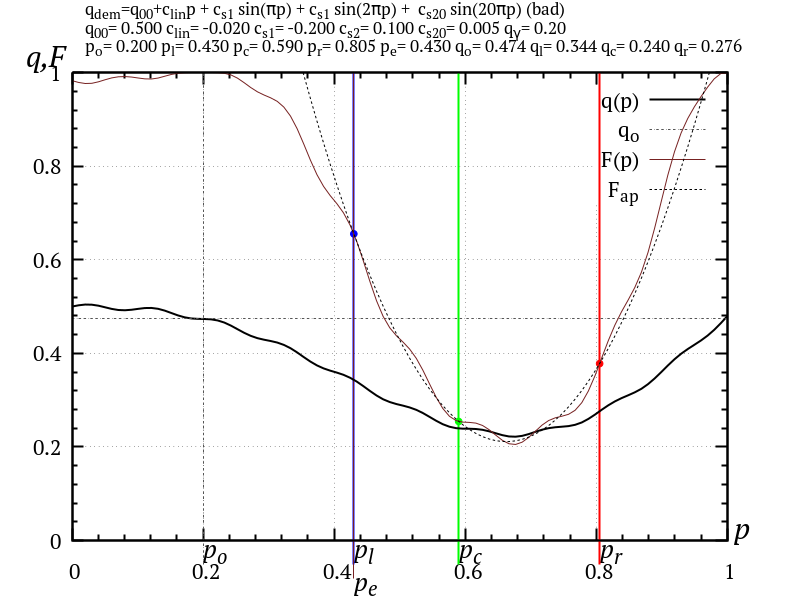
\includegraphics[width=60\TW]{p/p_eFq/q_p_eFq_bad.png}}
  \caption{Определение точки $p_e$ методом $p_{eFq}$ в худшем случае}
  \label{atu:f:p_eFq_bad}
\end{figure}

Как видно из графика, в этом случае аппроксимация зависимости $F(p)$
параболой $F_{ap}(p)$ достаточно точная, но положительная определённость величины
$a_2$ показывает, что найденный экстремум соответствует минимуму,
что совершенно не помогает в определении $p_e$. В то же время,
действие метода в этом случае --- выбор одной из граничных точек
правильно указывает направление.

Противоположный случай, когда центральная точка --- наилучшая,
но всё же недостаточно ``хорошая'', представлен на рис.~\ref{atu:f:p_eFq_good}.

\begin{figure}[htb!]
  \centerline{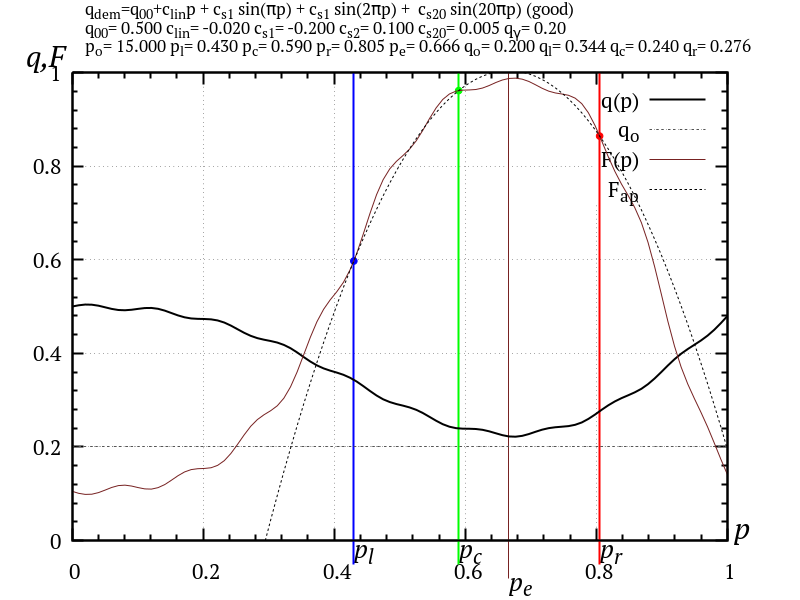
\includegraphics[width=60\TW]{p/p_eFq/q_p_eFq_good.png}}
  \caption{Определение точки $p_e$ методом $p_{eFq}$ в случае, когда центральная точка --- наилучшая, но нет пересечения $q(p)$ с $q_o$ }
  \label{atu:f:p_eFq_good}
\end{figure}

В отличие от метода $p_{eql}$, для рассматриваемого метода
этот случай не является особым. Найденное значение $p_e$
достаточно хорошо соответствует точке, в которой
$q(p)$ максимально приближается к $q_o$. Это вполне разумное поведение,
с учётом того, что при приближении к этой точке, по уточнённым данным
может быть найдено пересечение $q(p) = q_o$. С другой стороны,
это может быть локальный экстремум, не соответствующий искомому значению $p_o$,
как и представлено в этом примере.

Пример неопределённого случая, когда на рабочем интервале есть
два пересечения $q(p)$ с $q_o$, представлен на рис.~\ref{atu:f:p_eFq_double}.

\begin{figure}[htb!]
  \centerline{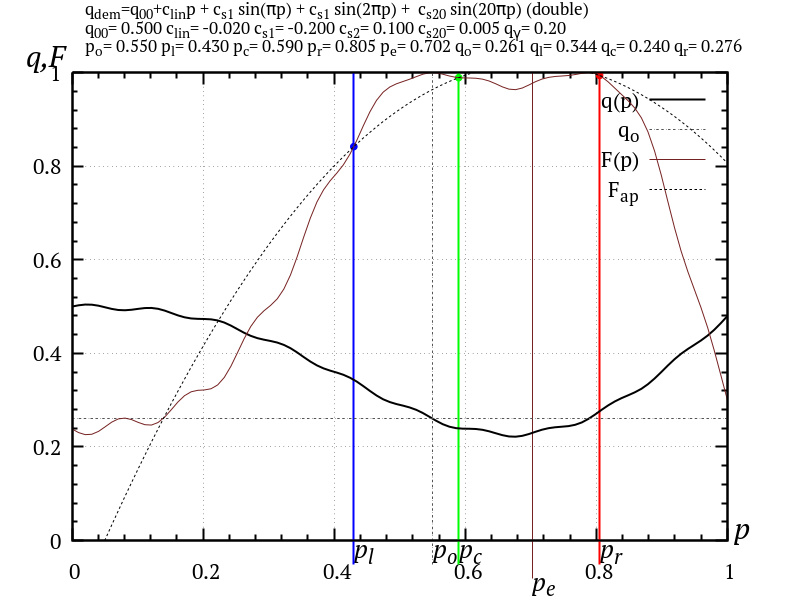
\includegraphics[width=60\TW]{p/p_eFq/q_p_eFq_double.png}}
  \caption{Определение точки $p_e$ методом $p_{eFq}$ в случае двух пересечений $q(p)$ с $q_o$ }
  \label{atu:f:p_eFq_double}
\end{figure}

Неопределённость условия не позволяет выбрать какое-либо определённое и
наилучшее в любом случае поведение. В данном конкретном случае
был выбран вариант, уводящий от исходного $p_o$.
Более того, в отличие от метода $p_{eql}$,
алгоритмически данный случай выделить невозможно, опираясь только на значения
функции качества. Как результат --- нет возможности отметить этот случай снижением
величины $S$.

Рассмотрим более определённый случай, для которого метод $p_{eql}$
получал оценку $p_e$ путём экстраполяции (рис.~\ref{atu:f:p_eFq_extra}).

\begin{figure}[htb!]
  \centerline{
    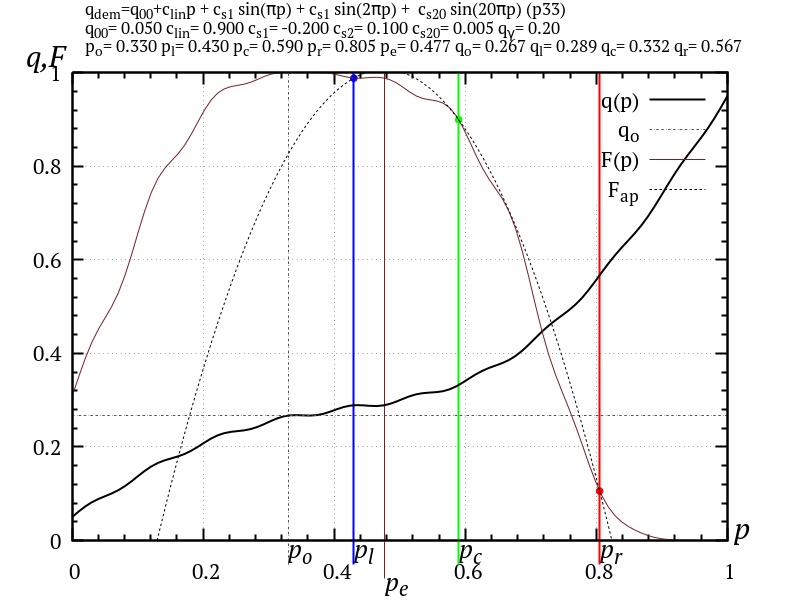
\includegraphics[width=49\TW]{p/p_eFq/q_p_eFq_p33.png}
    \hfill
    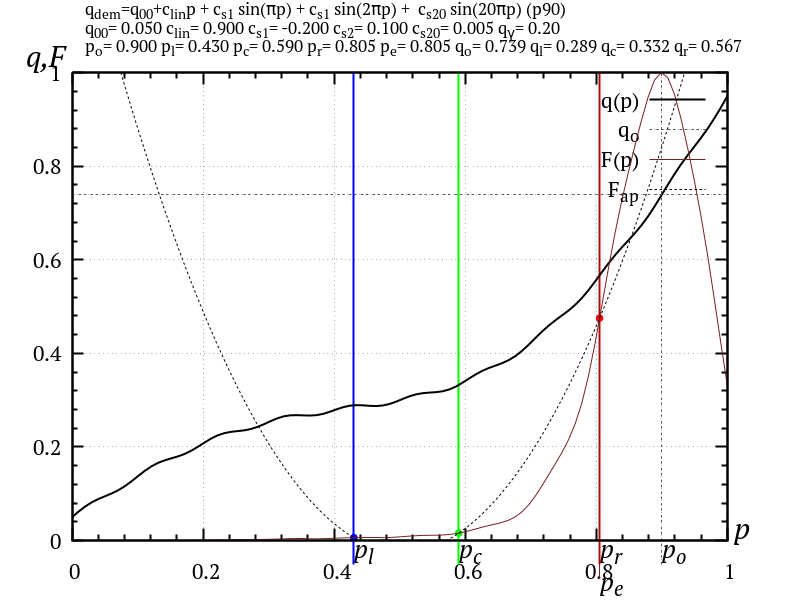
\includegraphics[width=49\TW]{p/p_eFq/q_p_eFq_p90.png}
  }
  \caption{Определение точки $p_e$ методом $p_{eFq}$ при экстраполяции за пределы $[p_l,p_r]$ }
  \label{atu:f:p_eFq_extra}
\end{figure}

Здесь наблюдаются серьёзные отличия от метода $p_{eql}$.
Прежде всего, поведение предыдущего метода
в этом, достаточно простом случае, было достаточно однозначным.
Достаточно было по заданным правилам уменьшать величину $S$
при удалении от рабочего интервала, для отображения
уменьшения степени уверенности в полученном значении.
Данный метод, как видно на представленных графиках,
в сходных случаях может давать совершенно различные результаты.
Первый график, соответствующий $p_o=0.33$,
демонстрирует не только значительную ошибку идентификации,
но и тот факт, что нет возможности отделить этот случай от
наиболее благоприятного, при $p_o \in [p_l,p_r]$.
Второй график ($p_o=0.9$), хотя исходные условия принципиально не отличаются
от первого, реализует условие $a_2 \ge 0 $, т.е. невозможность
определить $p_e$ за счёт аппроксимации второго порядка, и следовательно,
вынуждает в качестве приближения использовать $p_r$.

Действия метода в наиболее благоприятном случае, когда
 $p_o \in [p_l,p_r]$, представлены на рис.~\ref{atu:f:p_eFq_intra}.


\begin{figure}[htb!]
  \centerline{
    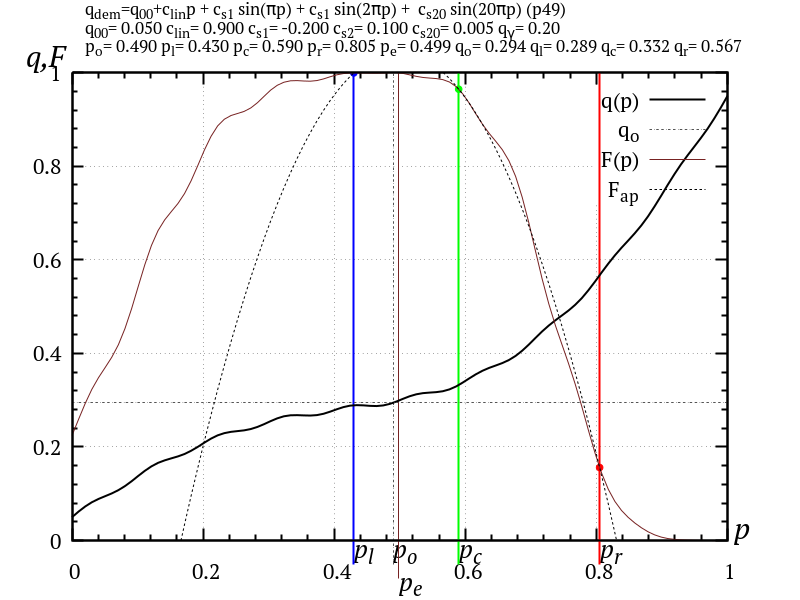
\includegraphics[width=49\TW]{p/p_eFq/q_p_eFq_p49.png}
    \hfill
    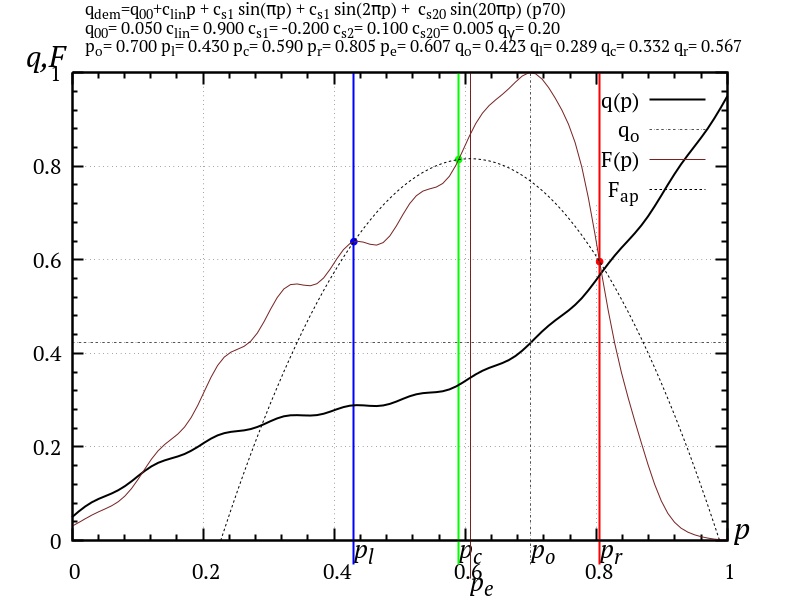
\includegraphics[width=49\TW]{p/p_eFq/q_p_eFq_p70.png}
  }
  \caption{Определение точки $p_e$ методом $p_{eFq}$ при   $p_o \in [p_l,p_r]$}
  \label{atu:f:p_eFq_intra}
\end{figure}

Как и следовало ожидать, оценка $p_e$ в этом случае вполне состоятельна,
несмотря на то, что в схожих условиях
наблюдается различный уровень ошибки идентификации.

Рассмотрим влияние на работоспособность рассматриваемого метода
чувствительности функции качества, определяемой величиной $q_\gamma$.
Исходное значение этой величины ($q_\gamma=0.2$) для
тестовой задачи было подобрано экспериментально~\cite{atu_asau22}.
Рассмотрим изменение результатов работы метода в при $p_o \in [p_l,p_r]$
в условиях сильно завышенной чувствительности $q_\gamma=0.05$ (рис.~\ref{atu:f:p_eFq_intra_005}).


\begin{figure}[htb!]
  \centerline{
    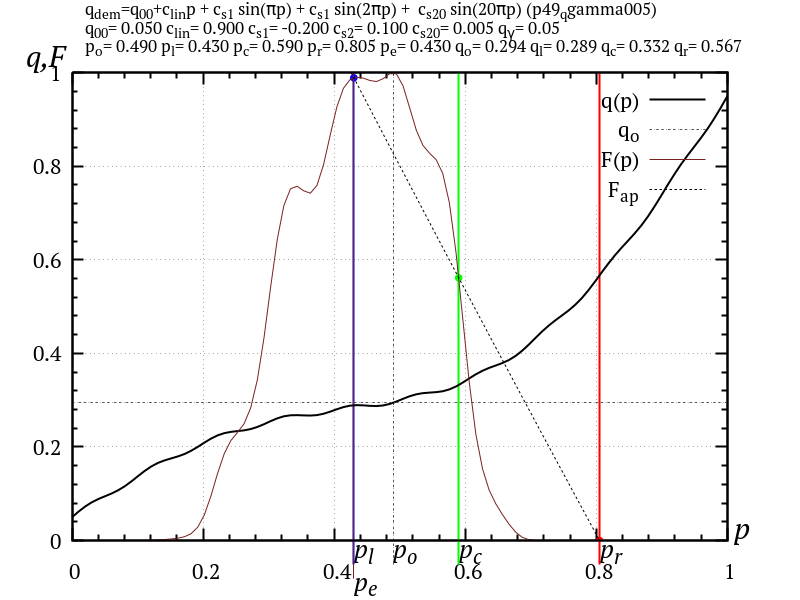
\includegraphics[width=49\TW]{p/p_eFq/q_p_eFq_p49_qgamma005.png}
    \hfill
    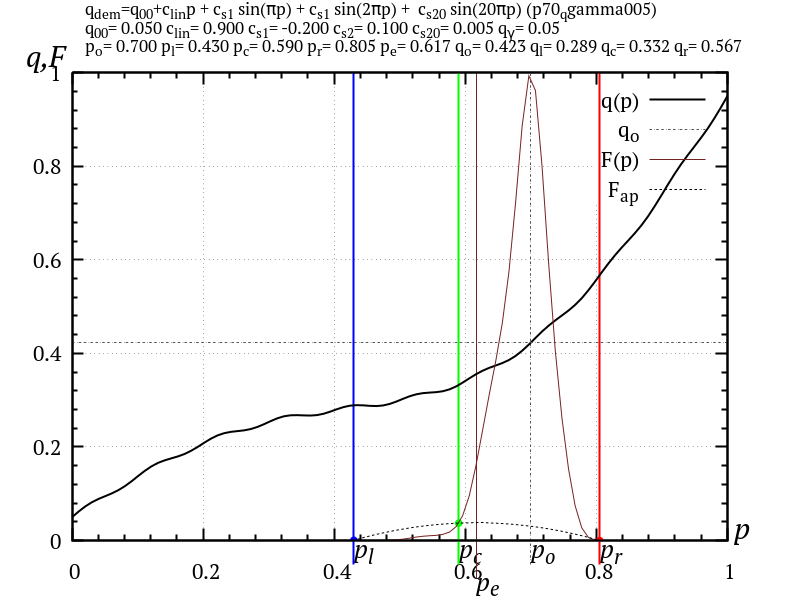
\includegraphics[width=49\TW]{p/p_eFq/q_p_eFq_p70_qgamma005.png}
  }
  \caption{Определение точки $p_e$ методом $p_{eFq}$ при завышенной чувствительности функции качества}
  \label{atu:f:p_eFq_intra_005}
\end{figure}

Как и следовало ожидать, избыточная чувствительность приводит к тому,
что функция качества отлична от нуля в очень узком диапазоне значений параметра,
что приводит к  практической бессмысленности используемой аппроксимации,
и неадекватным результатам идентификации.

Существенно другие результаты показывает метод в условиях
недостаточной чувствительности, то ест при
относительно больших значениях $q_\gamma$ (рис.~\ref{atu:f:p_eFq_intra_200}).

\begin{figure}[htb!]
  \centerline{
    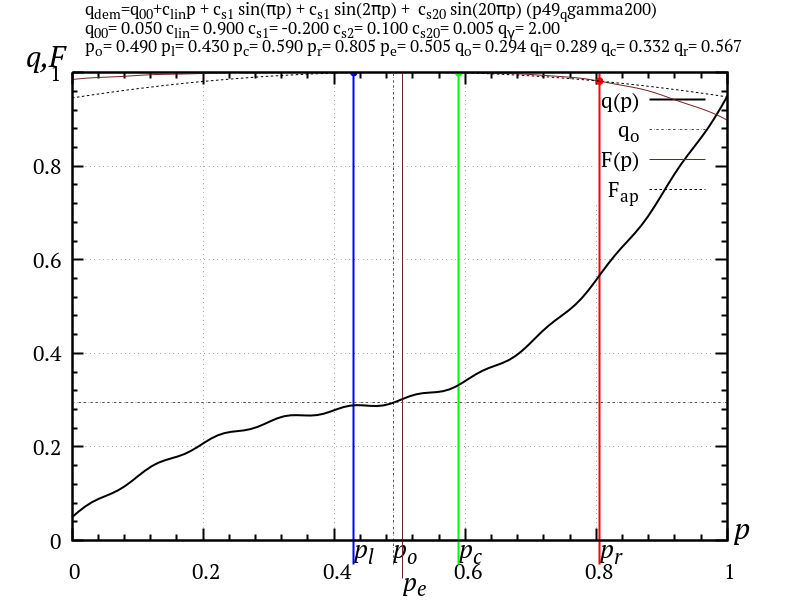
\includegraphics[width=49\TW]{p/p_eFq/q_p_eFq_p49_qgamma200.png}
    \hfill
    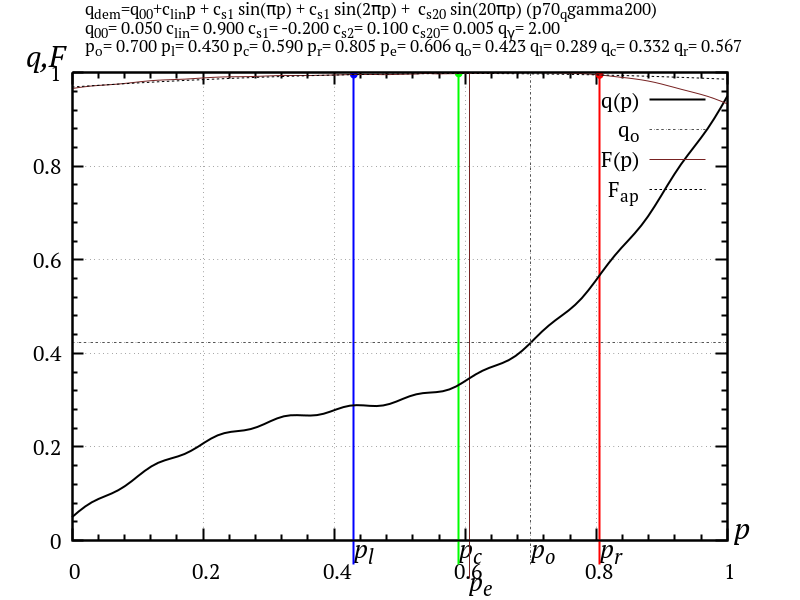
\includegraphics[width=49\TW]{p/p_eFq/q_p_eFq_p70_qgamma200.png}
  }
  \caption{Определение точки $p_e$ методом $p_{eFq}$ при недостаточной чувствительности функции качества}
  \label{atu:f:p_eFq_intra_200}
\end{figure}

Довольно странным является тот факт, что при значительном уменьшении
чувствительности ошибка идентификации растёт очень слабо.
В первую очередь это связано с тем, что в этих условиях
сама аппроксимация кривой Гаусса параболой становится более точной.
Для других видов функции качества это не так.
Более того, приведённые примеры рассчитывались при условии
отсутствия ошибок измерения. При недостаточной чувствительности
$F_l \approx F_c \approx F_r \approx 1$, и малые изменения $F$
приведут к значительной ошибке идентификации.

% TODO: good q_\gamma


В целом, на основании полученных результатов, можно данный метод
демонстрирует несколько худшие результаты, чем $p_{eql}$.
Наиболее серьёзным недостатком следует считать
невозможность в произвольном случае достаточно уверенно
определить величину $S$, которая на уровне координатора поиска
позволяет выбрать наиболее значимых агентов, а на уровне агента ---
избежать избыточной динамики вдали от $p_o$.
Вторым по важности недостатком является необходимость
корректной настройки величины $q_\gamma$, пусть и в достаточно широких пределах.
Среди достоинств метода следует отметить более простую
алгоритмическую организацию, что может быть существенно
при реализации системы идентификации в условиях с ограниченным вычислительными
ресурсами.



\paragraph{Определение $p_e$ методом COG по значениям функции качества в 3 точках}

Достаточно простым и малозатратным с точки зрения вычислений
является метод оценивания $p_e$ методом COG (``Center of gravity'')
по значениям функции качества:
%
\begin{equation}
  p_e =
  \frac{p_l F_l + p_c F_c + p_r F_r}{ F_r + F_c + F_r}  .
  \label{atu:eq:p_eFc}
\end{equation}

Условие ограниченности оценки
$p_e \in [p_l;p_r]$ в этом случае выполняется автоматически.
Единственная сложность --- обработка особого случая для тех видов
$F(q)$, которые обращаются в ноль на удалении от центральной точки.
В этом случае знаменатель (\ref{atu:eq:p_eFc}) обращается в ноль,
в в качестве $p_e$ имеет смысл выбрать $p_c$.
Для тех видов функций качества, которые не принимают строго нулевых
значений, формально такой проблемы нет. Нем не менее,
данное состояние сильно подвержено влиянию помех измерения.

Для этого способа не представляется возможным
достаточно полезным способом определить величину $S$,
поэтому, для сохранения единообразия положим $S=1$.

Определение $p_e$ по (\ref{atu:eq:p_eFc}) в дальнейшем будем обозначать $p_{eFc}$.



% }}}2

\subsection{Оценка работоспособности и эффективности методов оценивания идентифицируемого параметра одним поисковым агентом}  % {{{2

Для определения работоспособности и свойств различных методов оценивания $p_e$
в контролируемых условиях без учёта динамики агентов, была выбрана следующая
тестовая задача: зависимость $q(p)$ определялась по (\ref{atu:eq:q_dem}),
$p_{\min}=20$, $p_{\max}=60$,
$q_{00}=7$, $c_\mathrm{lin}=-4.0$.
Изначальное расположение агентов равномерное, и искусственно  зафиксированное:
$p_l=30$, $p_c=40$,  $p_r=50$.

Значения коэффициентов
$c_\mathrm{s1}$, $c_\mathrm{s2}$, $c_\mathrm{s20}$
выбирались по одному из трёх наборов:
%
\begin{equation}
  c_\mathrm{s1} = 0.2, c_\mathrm{s2} = -0.4, c_\mathrm{s20} = 0.02,
  \label{atu:eq:q_dem_all}
\end{equation}
%
\begin{equation}
  c_\mathrm{s1} = 0, c_\mathrm{s2} = 0, c_\mathrm{s20} = 0.02,
  \label{atu:eq:q_dem_s20}
\end{equation}
%
\begin{equation}
  c_\mathrm{s1} = c_\mathrm{s2} = c_\mathrm{s20} = 0 .
  \label{atu:eq:q_dem_lin}
\end{equation}

При этом набор параметров (\ref{atu:eq:q_dem_all})
позволяет исследовать поведение ошибки идентификации при
влиянии как низкочастотных, так и высокочастотных
нелинейных компонент,
(\ref{atu:eq:q_dem_s20}) --- только высокочастотных,
а (\ref{atu:eq:q_dem_lin}) представляет собой
простейший линейный случай.

\begin{figure}[htb!]
  \centerline{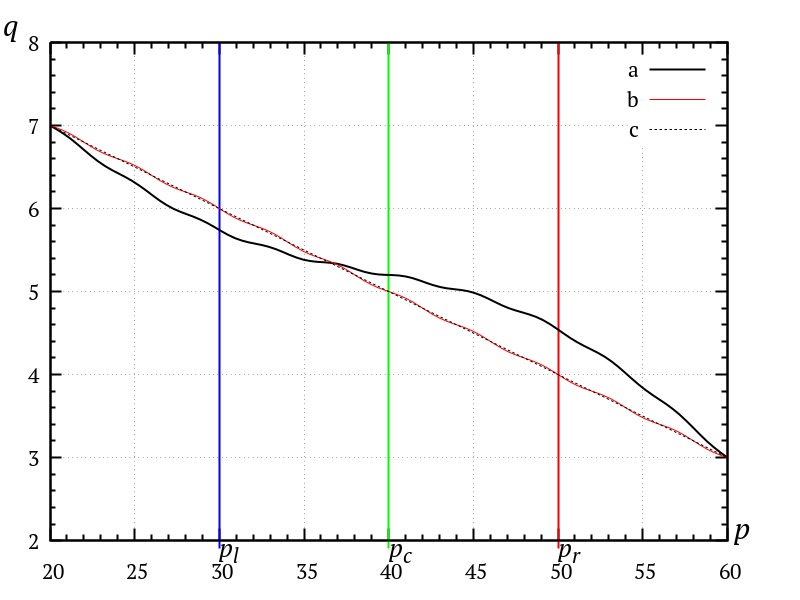
\includegraphics[width=0.7\textwidth]{p/q_p_dem.png} }
  \caption{Вид тестовой функции $q_\mathrm{dem}(p)$:
     a --- условия (\ref{atu:eq:q_dem_all}),
     b --- условия (\ref{atu:eq:q_dem_s20}),
     c --- условия (\ref{atu:eq:q_dem_lin})
  }
  \label{atu:f:q_dem}
\end{figure}

В первой серии вычислительных экспериментов
значение параметра объекта $p_o$
изменялось в диапазоне  $[ p_{\min}; p_{\max}]$
при фиксированном расстоянии между агентами $A = p_c - p_l = p_r - p_c$.
Это позволило оценить как интерполяционные (при $p_o \in [p_l,p_r] $),
так и экстраполяционные возможности методов. Так как
часть методов при определении $p_e$ использует значения
функции качества, то при проведении экспериментов
величина $q_\gamma$ также варьировалась.
Для метода $p_{eql}$ непосредственной зависимости от этой величины нет,
но для единообразия представленных результатов
все графики приведены как зависимости от $p_o$ и $q_\gamma$.
Все представленные графики, для удобства сравнения,
выполнены в одном масштабе и одной и той же проекции.
Масштаб по оси $Z$, использующейся для представления
модуля ошибки идентификации, был выбран $Z_{\max} = A/2 = 5$
для наглядного сравнения с расстоянием между агентами,
при этом величины, большие $A/2$ соответствуют
неоправданно большой ошибке, и находятся за пределами графика.

На рис.~\ref{atu:f:qsl_pe_po_qg_all} представлены зависимости ошибок идентификации
для тестовой задачи (\ref{atu:eq:q_dem})
при полном комплекте нелинейных членов (\ref{atu:eq:q_dem_all})
тремя неподвижными агентами тремя рассмотренным методами определения $p_e$.

\begin{figure}[htb!]
  \centerline{
    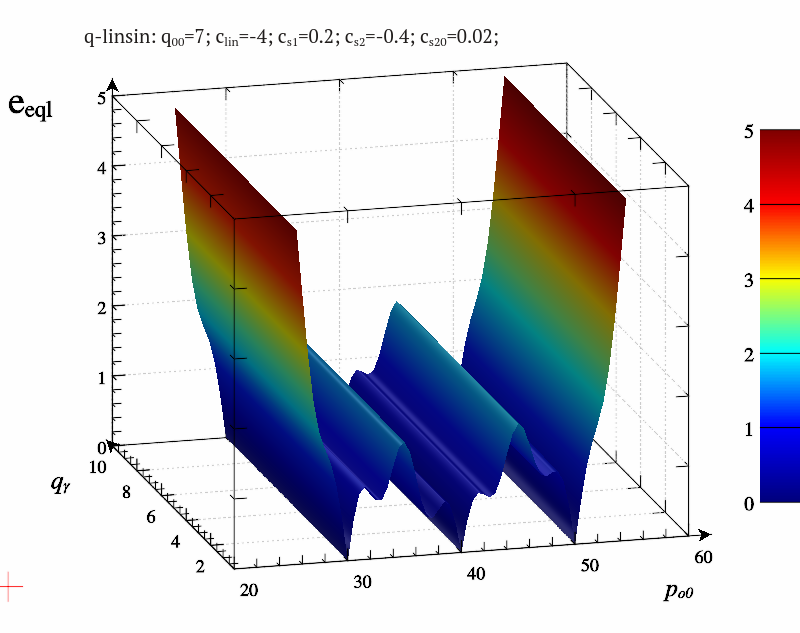
\includegraphics[width=0.32\textwidth]{p/qls_pe-p_po_qg_eql_all.png}
    \hfill
    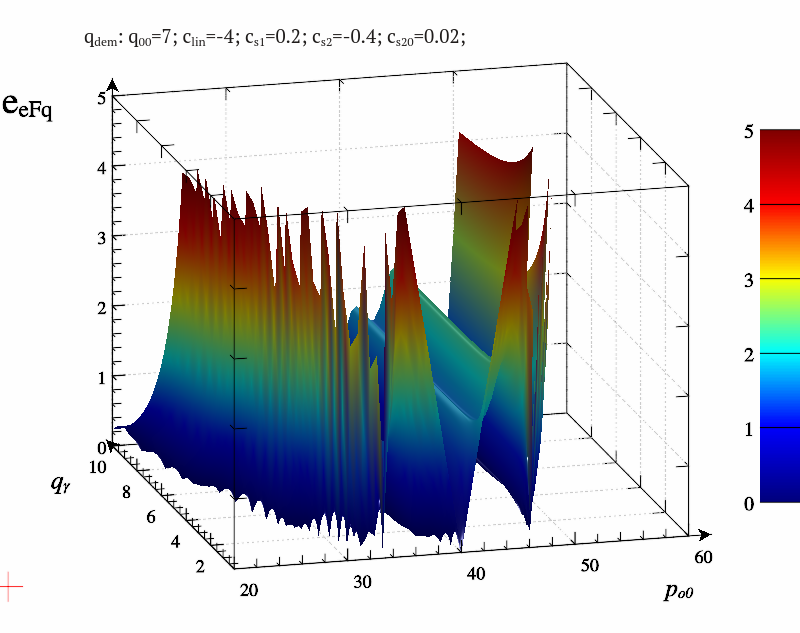
\includegraphics[width=0.32\textwidth]{p/qls_pe-p_po_qg_eFq_all.png}
    \hfill
    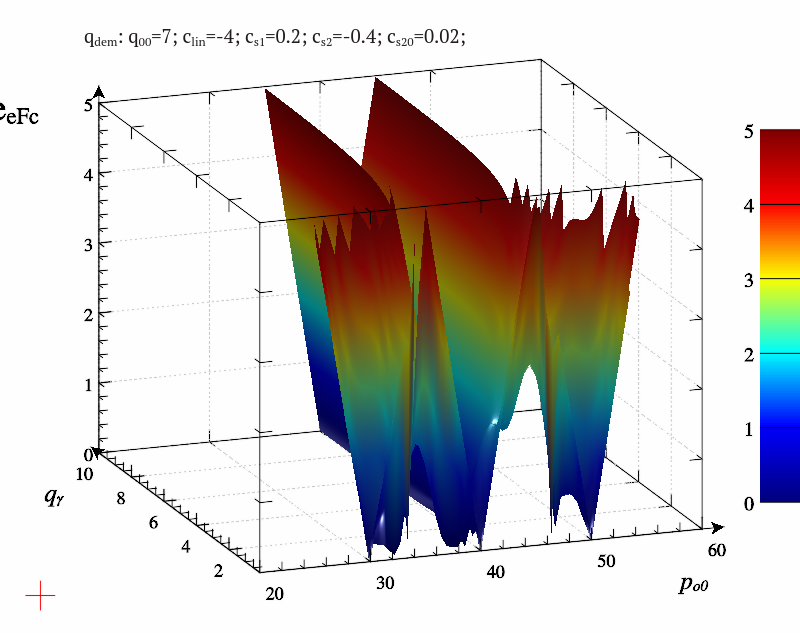
\includegraphics[width=0.32\textwidth]{p/qls_pe-p_po_qg_eFc_all.png}
  }
  \caption{Зависимости $e(p_o,q_\gamma)$ для методов $p_{eql}$, $p_{eFq}$, $p_{qFc}$ для условий (\ref{atu:eq:q_dem_all})}
  \label{atu:f:qsl_pe_po_qg_all}
\end{figure}

Метод $p_{eql}$ демонстрирует достаточно ограниченную ошибку идентификации
при $p_o \in [p_l; p_r]$, и достаточно быстрый, но линейно ограниченный рост ошибки
за пределами этого рабочего диапазона.
Метод $p_{eFq}$ обнаруживает существенную зависимость от величины $q_\gamma$:
малые значения % TODO define
приводят к существенному росту ошибки, а с дальнейшим ростом
уровень ошибки в пределах рабочего диапазона примерно
одного порядка с ошибкой в методе $p_{eql}$.
При этом, за пределами рабочего диапазона наблюдается более существенный рост ошибки.
Метод $p_{qFc}$ демонстрирует приемлемые результаты
только в очень узком диапазоне значений $q_\gamma$,
что ставит под серьёзное сомнение применимость этого метода
для реальных задач, так как при этом нет возможности предсказать
то значение этого параметра, при котором метод будет работоспособен.


На рис.~\ref{atu:f:qsl_pe_po_qg_s20} представлены аналогичные зависимости ошибок идентификации,
но из нелинейных членов оставлен самый высокочастотный (\ref{atu:eq:q_dem_s20}).

\begin{figure}[htb!]
  \centerline{
    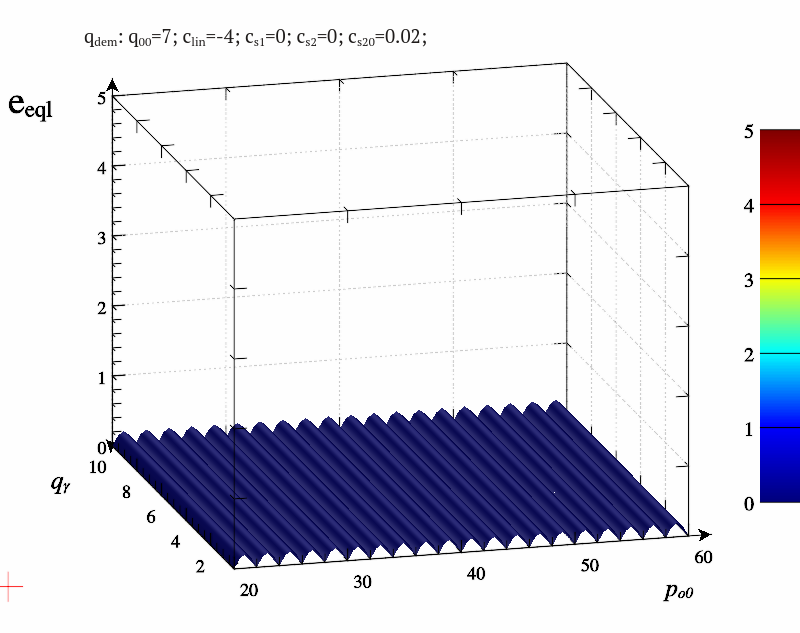
\includegraphics[width=0.32\textwidth]{p/qls_pe-p_po_qg_eql_s20.png}
    \hfill
    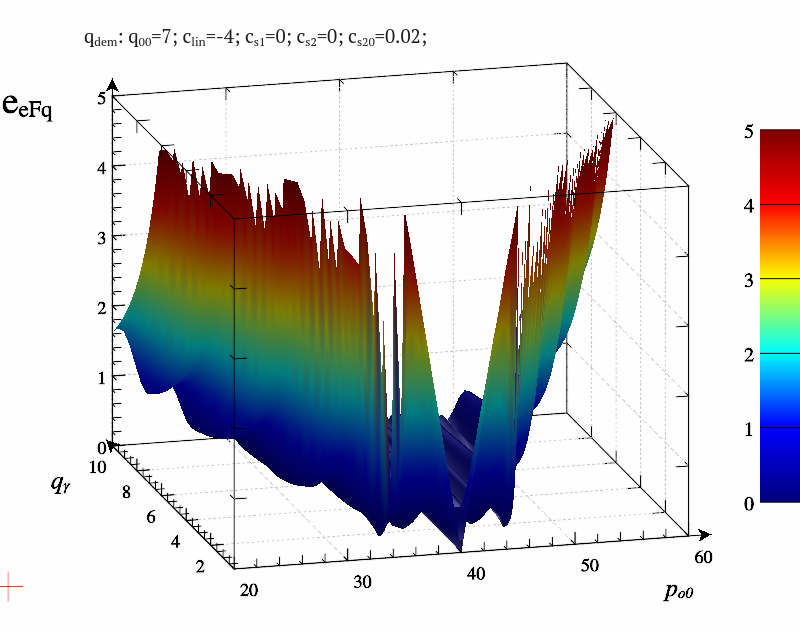
\includegraphics[width=0.32\textwidth]{p/qls_pe-p_po_qg_eFq_s20.png}
    \hfill
    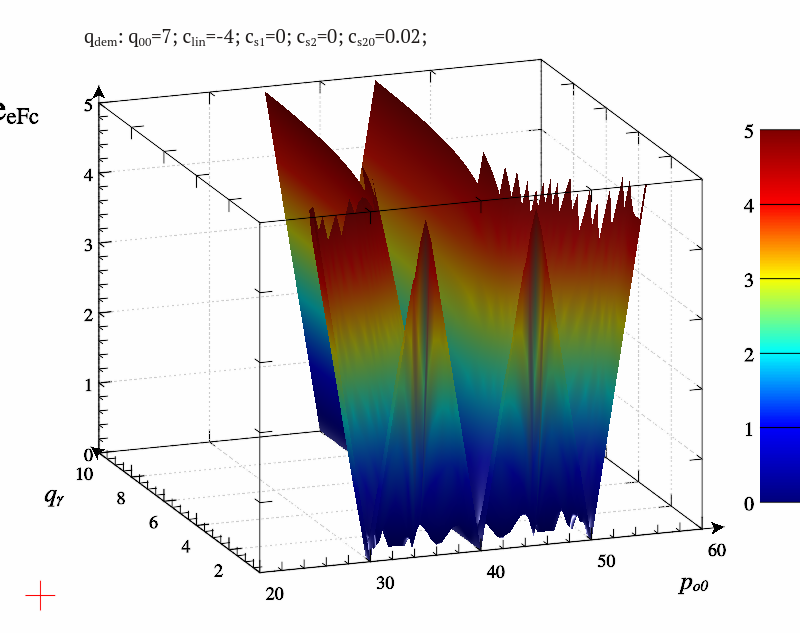
\includegraphics[width=0.32\textwidth]{p/qls_pe-p_po_qg_eFc_s20.png}
  }
  \caption{Зависимости $e(p_o,q_\gamma)$ для методов $p_{eql}$, $p_{eFq}$, $p_{qFc}$ для условий (\ref{atu:eq:q_dem_s20})}
  \label{atu:f:qsl_pe_po_qg_s20}
\end{figure}

В этих условиях метод $p_{eql}$ демонстрирует результаты, близкие к идеальным,
мелкая ``рябь'' на поверхности ошибки соответствует малым периодическим
возмущением $q(p)$, а в целом даже экстраполяция по приводит к росту ошибки.
В какой-то мере это обусловлено тем, что на рабочий диапазон приходится целое
число периодов возмущения. Зависимость ошибки для метода
$p_{eFq}$ проявляет меньшее значение ошибок для
тех участков, где и наблюдался небольшой уровень ошибок для
предыдущего случая, и практически неизменный --- в остальной области.
Принципиальной разницы в поведении метода $p_{qFc}$
по сравнению с предыдущим случаем нет.

На рис.~\ref{atu:f:qsl_pe_po_qg_lin} представлены те же зависимости,
в тривиальном случае (\ref{atu:eq:q_dem_lin}),
когда зависимость $q(p)$ линейна.

\begin{figure}[htb!]
  \centerline{
    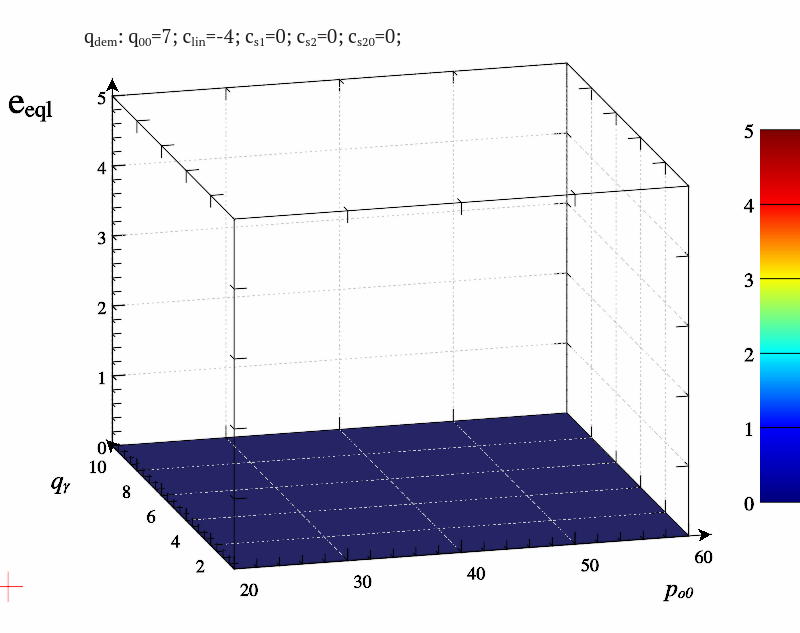
\includegraphics[width=0.32\textwidth]{p/qls_pe-p_po_qg_eql_lin.png}
    \hfill
    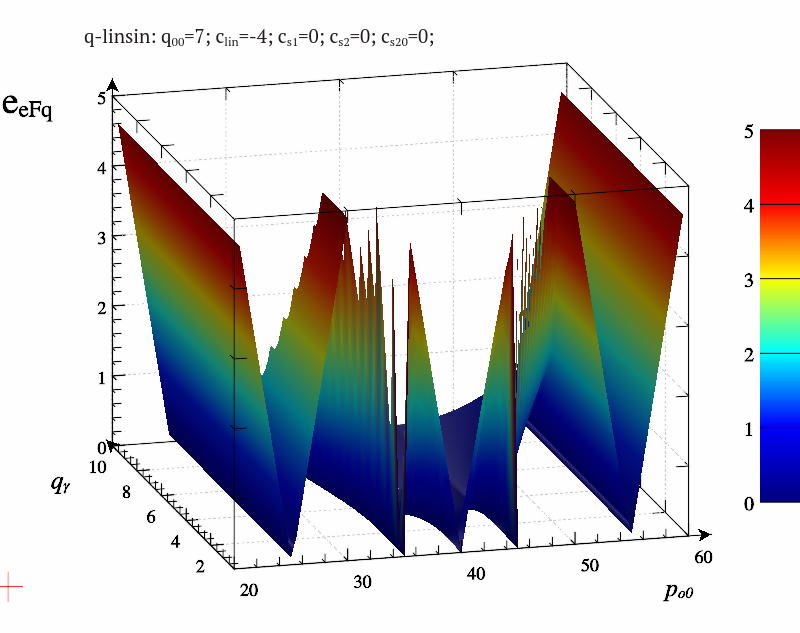
\includegraphics[width=0.32\textwidth]{p/qls_pe-p_po_qg_eFq_lin.png}
    \hfill
    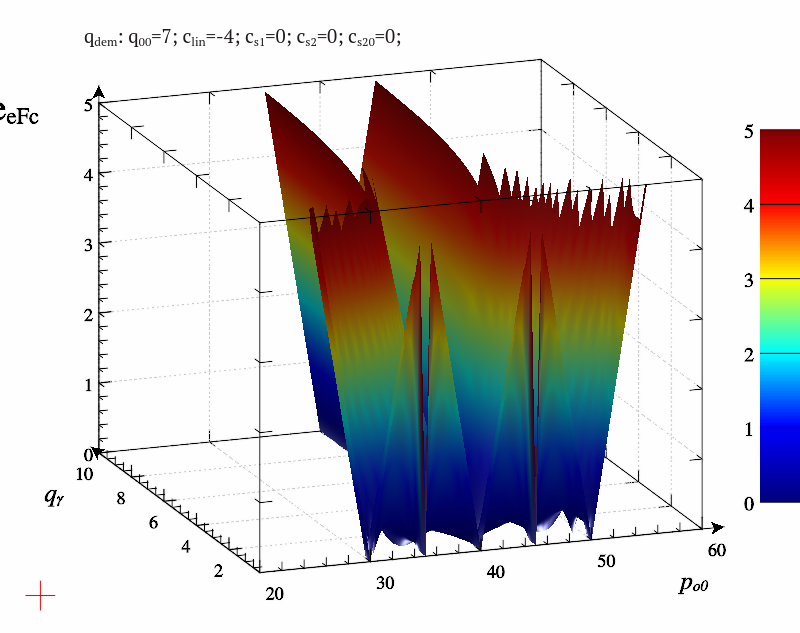
\includegraphics[width=0.32\textwidth]{p/qls_pe-p_po_qg_eFc_lin.png}
  }
  \caption{Зависимости $e(p_o,q_\gamma)$ для методов $p_{eql}$, $p_{eFq}$, $p_{qFc}$ для условий (\ref{atu:eq:q_dem_lin})}
  \label{atu:f:qsl_pe_po_qg_lin}
\end{figure}

Как и следовало ожидать, метод $p_{eql}$
демонстрирует идеальные результаты.
График зависимости для метода $p_{eFq}$
очерчивает его диапазон применимости --- несмотря
на линейность $q(p)$ метод становится неработоспособным при
излишне чувствительной функции качества.
И наконец, поверхность графика для метода $p_{eFc}$,
практически одинаковая для всех рассмотренных вариантов,
подтверждает его слабую применимость.



На рис.~\ref{atu:f:qsl_S_po_qg_all} представлены зависимости $S(p_o,q_\gamma)$
при полном комплекте нелинейных членов (\ref{atu:eq:q_dem_all}),
т.е. при тех же условиях, при которых был получен рис.~\ref{atu:f:qsl_pe_po_qg_all}.
Использовалось определение (\ref{atu:eq:S3}), как потенциально более
адекватное ошибке идентификации.

\begin{figure}[htb!]
  \centerline{
    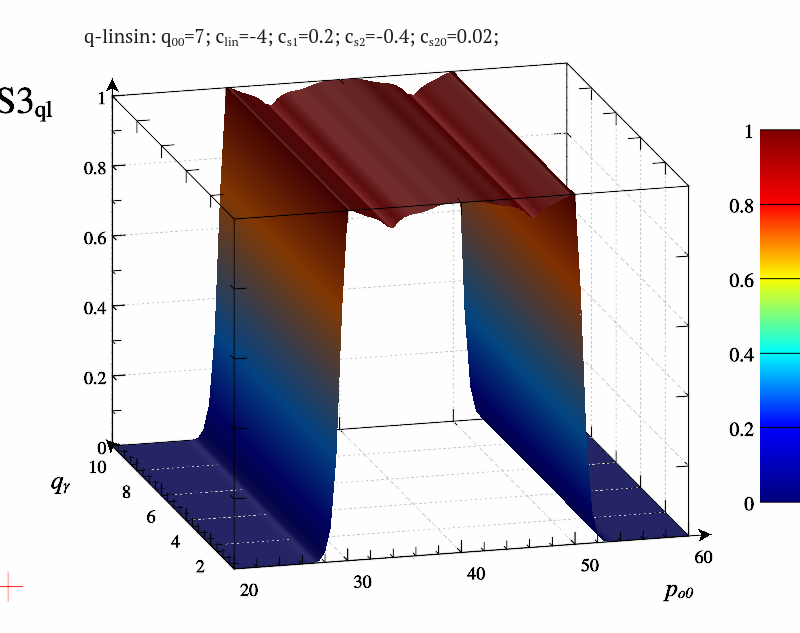
\includegraphics[width=0.32\textwidth]{p/qls_pe-p_po_qg_Sql_all.png}
    \hfill
    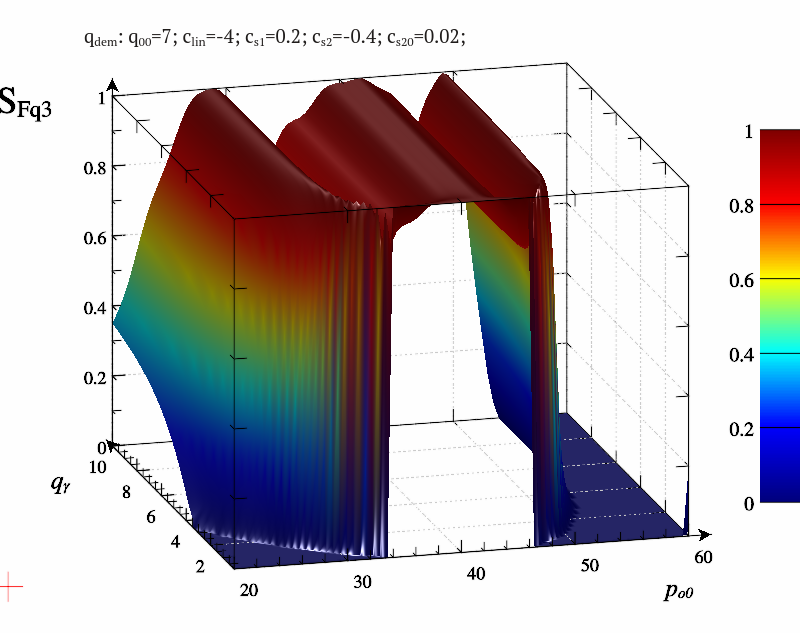
\includegraphics[width=0.32\textwidth]{p/qls_pe-p_po_qg_SFq_all.png}
    \hfill
    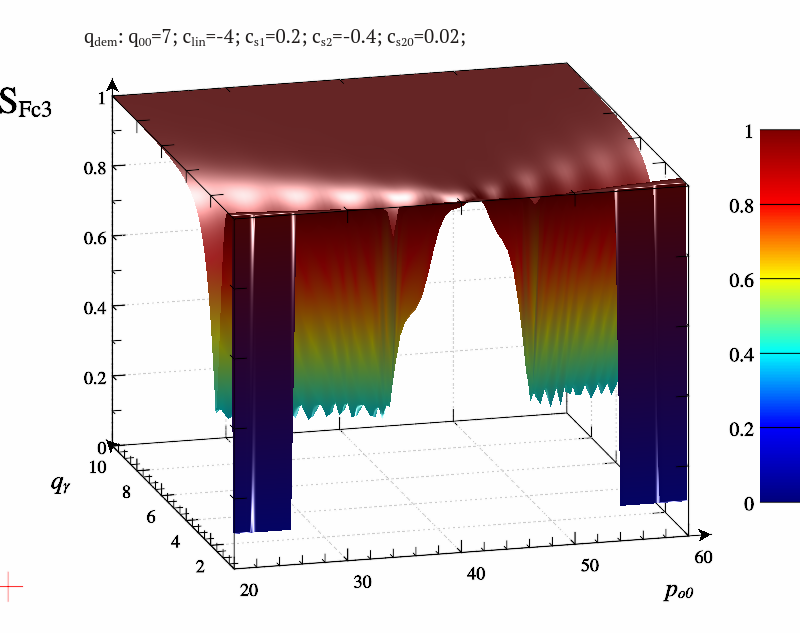
\includegraphics[width=0.32\textwidth]{p/qls_pe-p_po_qg_SFc_all.png}
  }
  \caption{Зависимости $S(p_o,q_\gamma)$ для методов $p_{eql}$, $p_{eFq}$, $p_{qFc}$ для условий (\ref{atu:eq:q_dem_all})}
  \label{atu:f:qsl_S_po_qg_all}
\end{figure}

Для метода $p_{eql}$ близкие к единице значения $S$, как и планировалось,
наблюдаются в тех же областях, где и низкий уровень ошибки идентификации,
в первую очередь --- внутри рабочего диапазона. При этом,
рассматриваемая величина не повторяет уровень ошибки, так как
это невозможно определить по трём точкам. Метод
$p_{eFq}$ также характеризуется достаточно осмысленным видом этой зависимости,
включая низкий уровень уверенности при завышенной чувствительности функции качества.
Напротив, для метода $p_{eFc}$ график показывает, что для него
данное определение $S$ не имеет смысла.


На рис.~\ref{atu:f:qsl_S_po_qg_s20} представлены аналогичные зависимости,
но из нелинейных членов оставлен самый высокочастотный (\ref{atu:eq:q_dem_s20}).

\begin{figure}[htb!]
  \centerline{
    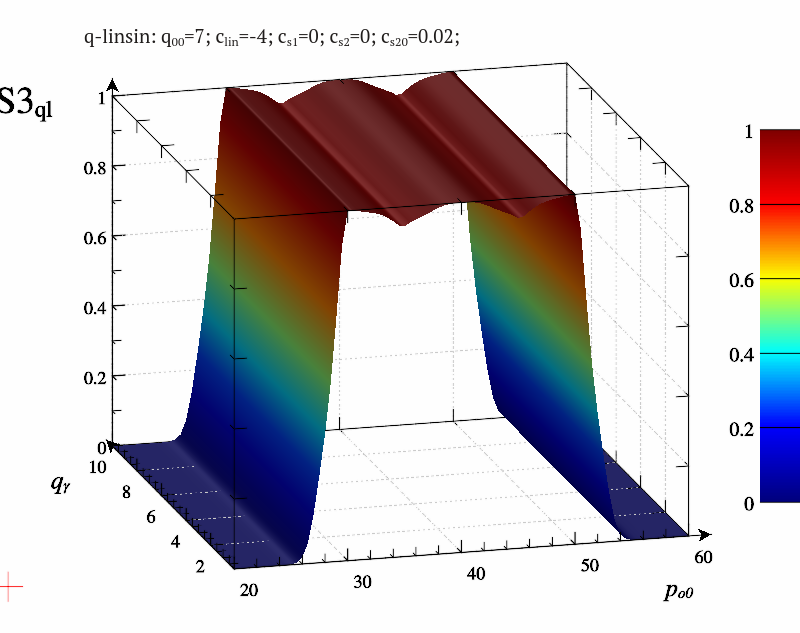
\includegraphics[width=0.32\textwidth]{p/qls_pe-p_po_qg_Sql_s20.png}
    \hfill
    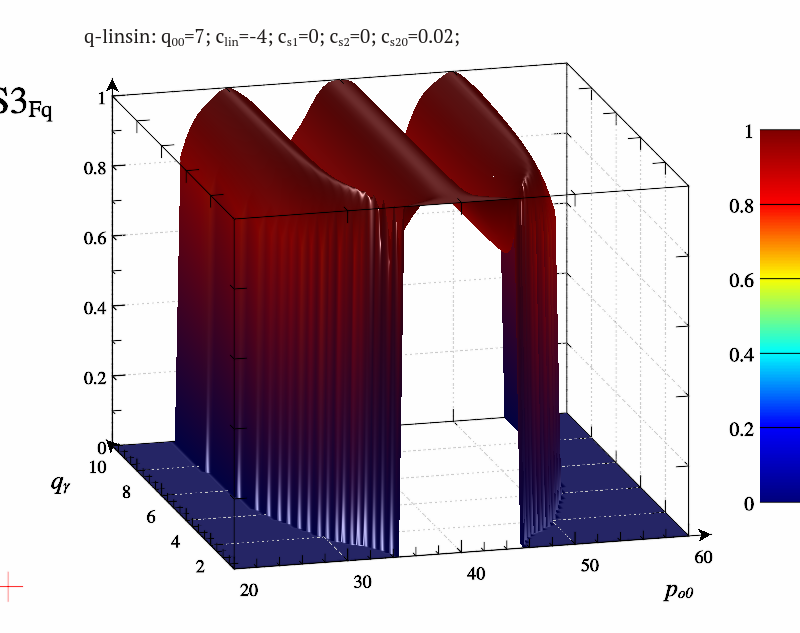
\includegraphics[width=0.32\textwidth]{p/qls_pe-p_po_qg_SFq_s20.png}
    \hfill
    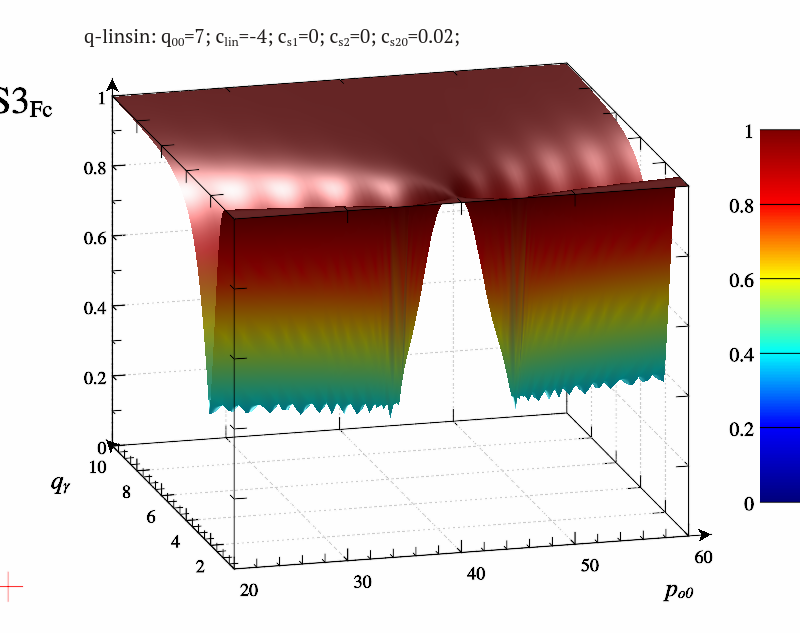
\includegraphics[width=0.32\textwidth]{p/qls_pe-p_po_qg_SFc_s20.png}
  }
  \caption{Зависимости $S(p_o,q_\gamma)$ для методов $p_{eql}$, $p_{eFq}$, $p_{qFc}$ для условий (\ref{atu:eq:q_dem_s20})}
  \label{atu:f:qsl_S_po_qg_s20}
\end{figure}

По сравнению с предыдущим случаем, график для метода $p_{eql}$
имеет ненамного больший охват, при сохранении общей формы.
Это связано с тем, что для данного случая $k_l=1$,
диапазон уверенного определения $p_e$ соответственно расширяется,
что даже избыточно подтверждается невозрастающим уровнем ошибок.
Изменения для метода $p_{qFq}$ не столь заметны,
так как для него не учитывается оценка уровня линейности.
Для метода $p_{eFc}$ сохраняется бессмысленная зависимость.

На рис.~\ref{atu:f:qsl_S_po_qg_lin} представлены те же зависимости зависимости,
но в линейном случае (\ref{atu:eq:q_dem_lin}).

\begin{figure}[htb!]
  \centerline{
    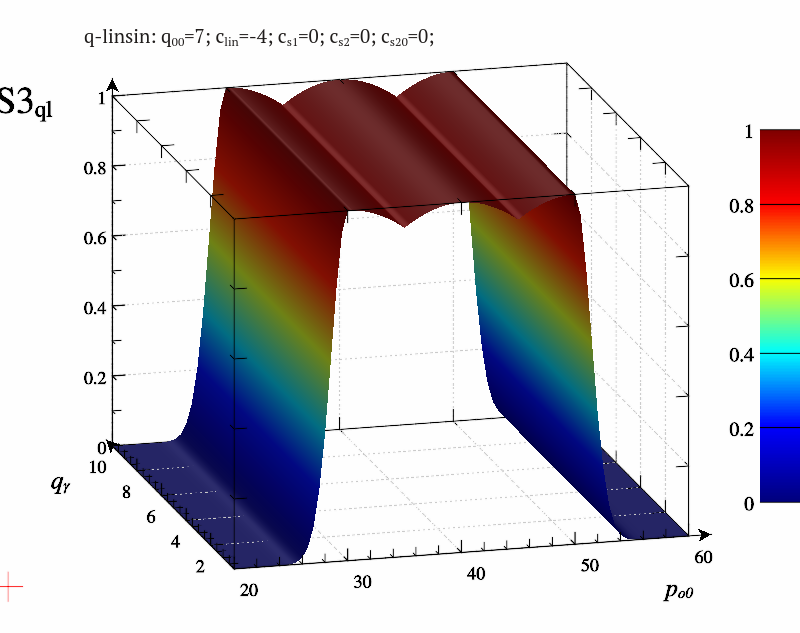
\includegraphics[width=0.32\textwidth]{p/qls_pe-p_po_qg_Sql_lin.png}
    \hfill
    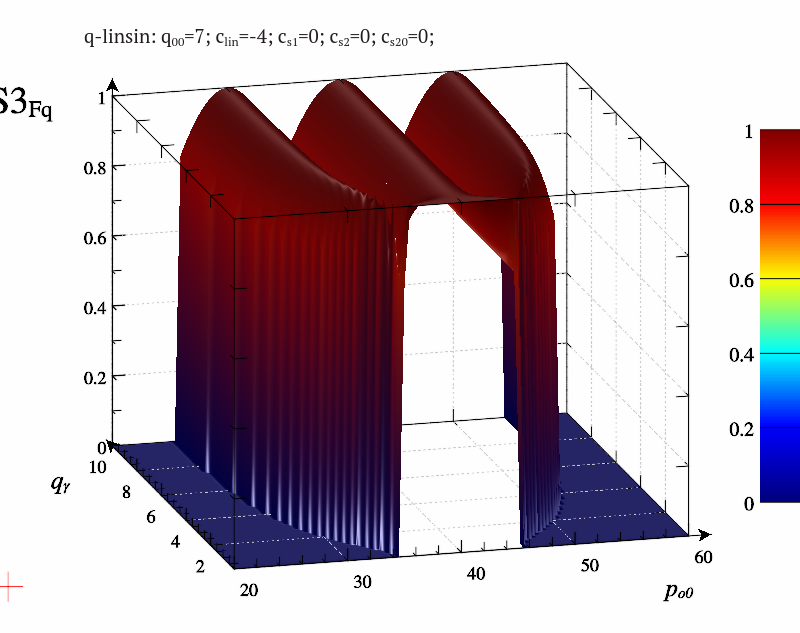
\includegraphics[width=0.32\textwidth]{p/qls_pe-p_po_qg_SFq_lin.png}
    \hfill
    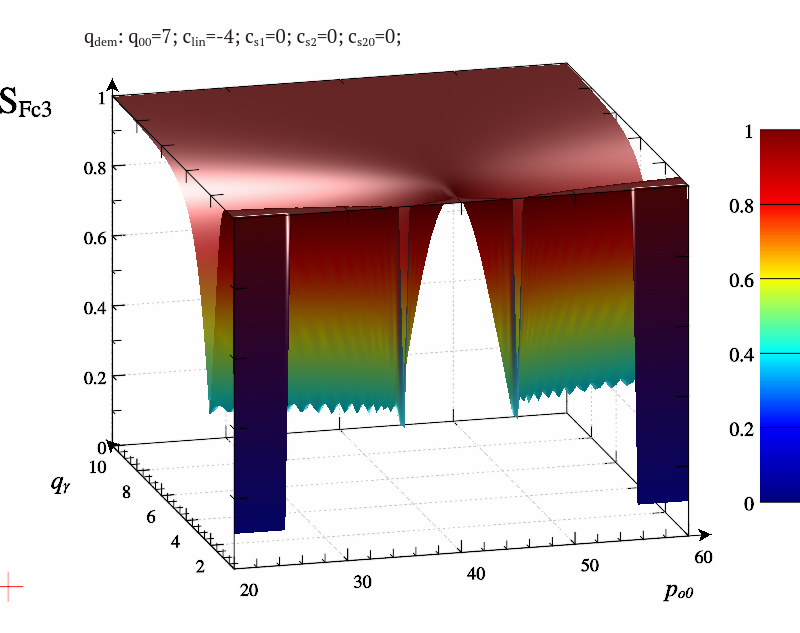
\includegraphics[width=0.32\textwidth]{p/qls_pe-p_po_qg_SFc_lin.png}
  }
  \caption{Зависимости $S(p_o,q_\gamma)$ для методов $p_{eql}$, $p_{eFq}$, $p_{qFc}$ для условий (\ref{atu:eq:q_dem_lin})}
  \label{atu:f:qsl_S_po_qg_lin}
\end{figure}

Принципиальной разницы с предыдущими графиками нет, так отличие
в условиях проявляется на относительно мелком масштабе,
и не влияет на довольно грубую оценку $S$.

На рис.~\ref{atu:f:qsl_W_po_qg_all}, \ref{atu:f:qsl_W_po_qg_s20}, \ref{atu:f:qsl_W_po_qg_lin},
представлены зависимости $W(p_o,q_\gamma)$
для всех рассмотренных вариантов.

\begin{figure}[htb!]
  \centerline{
    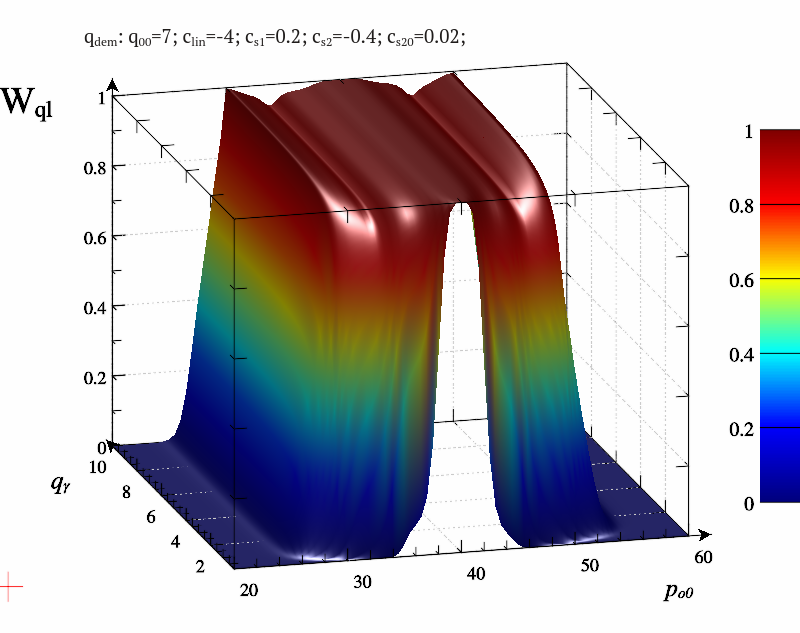
\includegraphics[width=0.32\textwidth]{p/qls_pe-p_po_qg_Wql_all.png}
    \hfill
    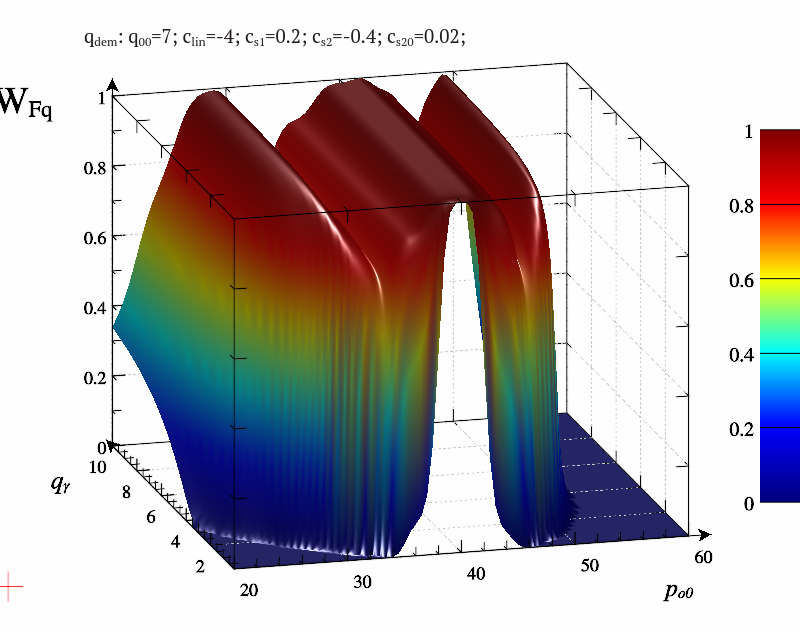
\includegraphics[width=0.32\textwidth]{p/qls_pe-p_po_qg_WFq_all.png}
    \hfill
    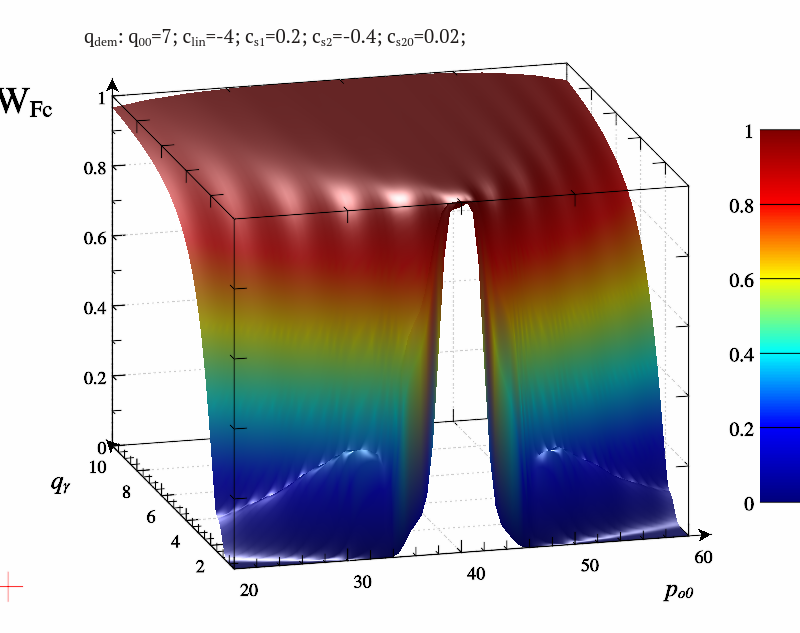
\includegraphics[width=0.32\textwidth]{p/qls_pe-p_po_qg_WFc_all.png}
  }
  \caption{Зависимости $W(p_o,q_\gamma)$ для методов $p_{eql}$, $p_{eFq}$, $p_{qFc}$ для условий (\ref{atu:eq:q_dem_all})}
  \label{atu:f:qsl_W_po_qg_all}
\end{figure}


\begin{figure}[htb!]
  \centerline{
    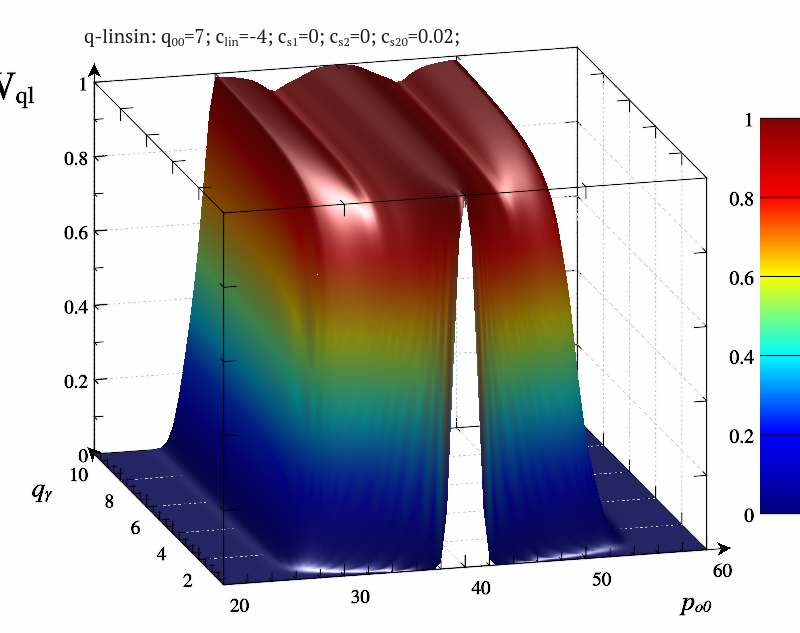
\includegraphics[width=0.32\textwidth]{p/qls_pe-p_po_qg_Wql_s20.png}
    \hfill
    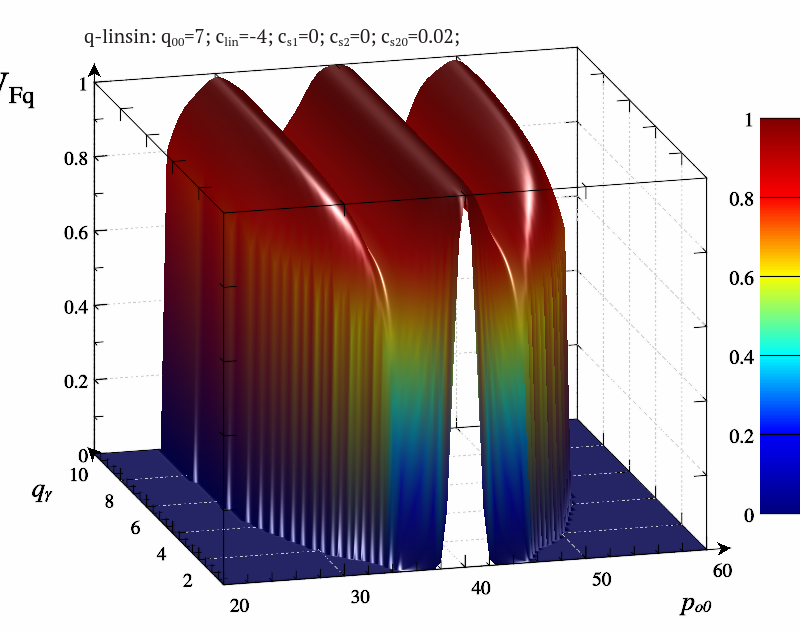
\includegraphics[width=0.32\textwidth]{p/qls_pe-p_po_qg_WFq_s20.png}
    \hfill
    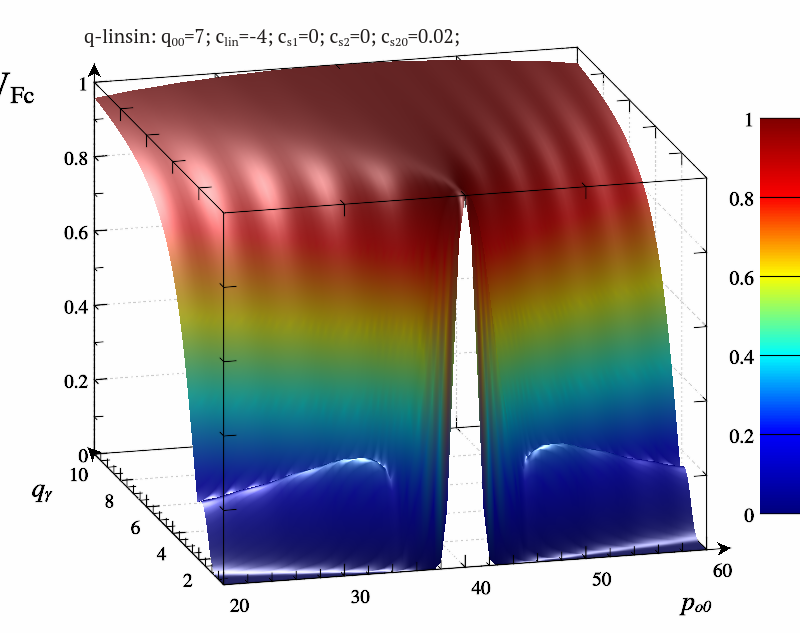
\includegraphics[width=0.32\textwidth]{p/qls_pe-p_po_qg_WFc_s20.png}
  }
  \caption{Зависимости $W(p_o,q_\gamma)$ для методов $p_{eql}$, $p_{eFq}$, $p_{qFc}$ для условий (\ref{atu:eq:q_dem_s20})}
  \label{atu:f:qsl_W_po_qg_s20}
\end{figure}

\begin{figure}[htb!]
  \centerline{
    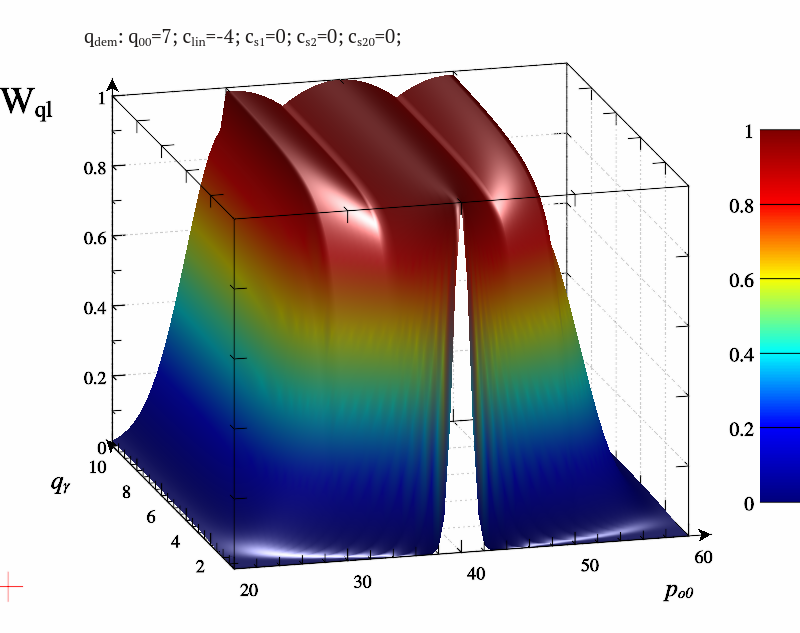
\includegraphics[width=0.32\textwidth]{p/qls_pe-p_po_qg_Wql_lin.png}
    \hfill
    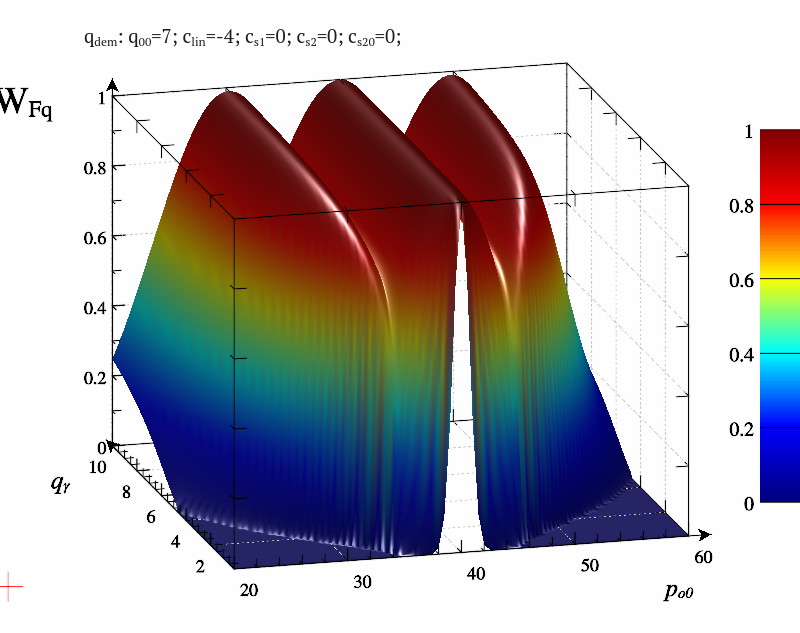
\includegraphics[width=0.32\textwidth]{p/qls_pe-p_po_qg_WFq_lin.png}
    \hfill
    \includegraphics[width=0.32\textwidth]{p/qls_pe-p_po_qg_WFc_lin.png}
  }
  \caption{Зависимости $W(p_o,q_\gamma)$ для методов $p_{eql}$, $p_{eFq}$, $p_{qFc}$ для условий (\ref{atu:eq:q_dem_lin})}
  \label{atu:f:qsl_W_po_qg_lin}
\end{figure}

Наиболее серьезное отличие от зависимостей $S(p_o,q_\gamma)$ наблюдается
для метода $p_{eql}$ --- начинает играть роль ``штраф'' за
избыточную чувствительность функции качества, которая в самом методе
практически не используется. Однако, для рассматриваемой области,
вблизи рабочего диапазона, отличие $W$ от $S$ не имеет особого значения.
Основное предназначение $W$ --- ограничивать динамику агентов,
находящихся вдали от искомого значения~$p_o$.


Во второй серии вычислительных экспериментов
значение параметра объекта
было фиксированным $p_o=39$,
а расстояние между агентами $A$
изменялось от $0.1$ до $20$.
При этом, при $A<1$
точка $p_o$ находилась за пределами интервала $[p_l,p_r]$,
и положение $p_e$ определялось с помощью экстраполяции.
Значительная часть этих графиков отображает противоположный случай ---
$p_O \in [p_l, p_r]$, и значение $p_e$ определяется
интерполяцией на расширяющемся (с ростом $A$) диапазоне.

На рис.~\ref{atu:f:qsl_pe_A_qg_all} представлены поверхности зависимости ошибок идентификации
при наличии всех нелинейных членов.


\begin{figure}[htb!]
  \centerline{
    \includegraphics[width=0.32\textwidth]{p/qls_pe-p_A_qg_eql_all.png}
    \hfill
    \includegraphics[width=0.32\textwidth]{p/qls_pe-p_A_qg_eFq_all.png}
    \hfill
    \includegraphics[width=0.32\textwidth]{p/qls_pe-p_A_qg_eFc_all.png}
  }
  \caption{Зависимости $e(A,q_\gamma)$ для методов $p_{eql}$, $p_{eFq}$, $p_{qFc}$ для условий (\ref{atu:eq:q_dem_all})}
  \label{atu:f:qsl_pe_A_qg_all}
\end{figure}

Для метода $p_{eql}$
форма этого графика достаточно предсказуема --- нет зависимости от $q_\gamma$,
на участке экстраполяции величина ошибки линейно падает при $A \to p_c - p_o$. При дальнейшем росте $A$
ошибка умеренно растёт, причём в этом росте можно выделить два участка.
Первый характеризуется относительно резким ростом ошибки, связанным
с увеличением влияние высокочастотных нелинейных членов,
второй --- достаточно плавным подъемом.

График, соответствующий методу $p_{eFq}$ проявляет явную зависимость
ошибки от $q_\gamma$. Для широкого диапазона величины $A$
существует достаточно узкая область значений $q_\gamma$,
при которых ошибка минимальна. Как избыточная, так и недостаточная чувствительность
функции качества приводит к росту ошибки. К сожалению,
даже для простейших случаев, подобных рассматриваемому,
получение аналитической зависимости этой области затруднено.
Также этот график отличается меньшей ошибкой в режиме экстраполяции,
но в целом этот метод проигрывает предыдущему.

График ошибки для метода $p_{eFc}$ подчёркивает ограниченную применимость этого метода.
Аналогично предыдущему методу, существует область наиболее благоприятных для
проведения идентификации значений $q_\gamma$. Однако,
уровень ошибки практически не падает при $p_l \to p_o$,
то есть этот метод не выигрывает в точности при концентрации
агентов в окрестности $p_o$.

Графики (рис.~\ref{atu:f:qsl_pe_A_qg_s20}), построенные с использованием
только высокочастотных нелинейных членов,
подтверждают представленные выше предположения
о влиянии нелинейностей различного частотного масштаба
на ошибку идентификации.

\begin{figure}[htb!]
  \centerline{
    \includegraphics[width=0.32\textwidth]{p/qls_pe-p_A_qg_eql_s20.png}
    \hfill
    \includegraphics[width=0.32\textwidth]{p/qls_pe-p_A_qg_eFq_s20.png}
    \hfill
    \includegraphics[width=0.32\textwidth]{p/qls_pe-p_A_qg_eFc_s20.png}
  }
  \caption{Зависимости $e(A,q_\gamma)$ для методов $p_{eql}$, $p_{eFq}$, $p_{qFc}$ для условий (\ref{atu:eq:q_dem_s20})}
  \label{atu:f:qsl_pe_A_qg_s20}
\end{figure}

При этом метод $p_{eql}$ характеризуется практическим отсутствием роста
ошибки как в режиме экстраполяции, так и при значительном росте $A$.
Метод $p_{eFq}$ также характеризуется существенно меньшим ростом
ошибки, за исключением области избыточной чувствительности.
Вид графика для метода $p_{eFc}$ практически не изменился.

В идеальном случае, при линейной зависимости $q_\mathrm{dem}(p)$~(рис.~\ref{atu:f:qsl_pe_A_qg_lin}),
метод $p_{eql}$ демонстрирует идеальные результаты.
Следует отметить, что в данной тестовой задаче отсутствуют
ошибки измерения.
Метод $p_{eFq}$ позволяет достичь пренебрежимо малой, но не нулевой
ошибки везде, за исключением области экстраполяции и завышенной чувствительности.
При этом, уровень ошибок даже в неблагоприятных областях
относительно мал. Напротив, метод $p_{eFc}$,
даже в идеальных условиях продолжает показывать
посредственные результаты.

\begin{figure}[htb!]
  \centerline{
    \includegraphics[width=0.32\textwidth]{p/qls_pe-p_A_qg_eql_lin.png}
    \hfill
    \includegraphics[width=0.32\textwidth]{p/qls_pe-p_A_qg_eFq_lin.png}
    \hfill
    \includegraphics[width=0.32\textwidth]{p/qls_pe-p_A_qg_eFc_lin.png}
  }
  \caption{Зависимости $e(A,q_\gamma)$ для методов $p_{eql}$, $p_{eFq}$, $p_{qFc}$ для условий (\ref{atu:eq:q_dem_lin})}
  \label{atu:f:qsl_pe_A_qg_lin}
\end{figure}

Таким образом, на основании результатов моделирования
можно сделать выводы о применимости рассмотренных методов:

\begin{itemize}

  \item
    Метод $p_{eFc}$ имеет предельно ограниченную применимость,
    единственные преимущества --- простота реализации,
    отсутствие особых случаев и естественная ограниченность
    $p_e$ не компенсируют все недостатки, поэтому в
    дальнейших исследованиях в данной этот метод применяться не будет.

  \item
    При нормальном функционировании метод $p_{eql}$
    обеспечивает лучшие результаты. При этом он сложнее
    в реализации, требует обработки ряда особых случаев.

  \item
    Метод $p_{eFq}$ демонстрирует результаты,
    сравнимые с методом $p_{eql}$, при этом
    он проще в реализации. В тех случаях,
    когда величина критерия самому агенту непосредственно не известна,
    этот метод, в отличие от методов, основанных и аппроксимации $q(p)$,
    сохраняет работоспособность. Недостатком является существенная зависимость от
    величины $q_\gamma$, однако, даже методы, которые
    не используют функцию качества на уровне агента, все равно
    применяют её на уровне координатора поиска, и задача выбора адекватной величины $q_\gamma$
    всё равно остаётся.

  \item
    Методы $p_{eql}$ и $p_{qFq}$ позволяет достичь меньшей ошибки идентификации
    при сближении поисковых агентов к $p_o$, при условии $p_o \in [p_l,p_r]$.
    Следовательно, для повышения точности идентификации необходимо
    или реализовывать поисковую динамику объекта, или же
    наращивать количество неподвижных агентов, что может быть недостижимо в условиях ограниченности
    ресурсов.


\end{itemize}




% }}}2

\subsection{Динамика поисковых агентов}  % {{{2

Значение $p_e$, полученное поисковым агентом, может использоваться непосредственно и
мгновенно в качестве значения параметров для управляемых моделей только в том случае,
если объект, и следовательно модели, не проявляют собственной динамики,
то есть являются статическими. Идентификация статических объектов не
является задачей в данной работе.

При моделировании произвольной нелинейной динамической системы,
а особенно хаотических систем, нет возможности строго
определить допустимую динамику изменения параметров
в процессе идентификации. Более того, существуют
даже линейные системы, для которых малые, но специальным
образом подобранные параметрические воздействия
приводят к неограниченному росту значений, отображающих
состояние системы. Одним из самых известных примеров
такого поведения является параметрический резонанс~\Cmt{ref:Sivuhin1}.
Для систем динамического хаоса более известным явлением является
сигнальная синхронизация систем, однако,
возможность аналогичных параметрических влияний достаточно очевидна.

Тем не менее, если исключить достаточно редкие особые случаи,
можно оценить допустимую динамику изменения параметров.
Прежде всего, в процессе синтеза критерия идентификации
одним из этапов является определение корректного значения $\tau_q$.
Чаще всего, данная величина неявно задаёт и допустимую
скорость изменения параметров моделей в процессе идентификации.

При моделировании динамики тела без учёта вращения в механике достаточно
задать все силы, действующие на это тело.
Аналогично, определяя  поисковую динамику агента
требуется определить эквивалент ``сил'',
вызывающих смещение параметров моделей, контролируемых агентом.
При этом задачу определения динамики можно упростить,
разделив ``силы'' на две группы. В первую входят
силы, приводящие к ``движению''. Во вторую входят силы сопротивления,
и вместо рассмотрения самих сил достаточно
определить правила динамики, при этом возможно
использование правил, не имеющих прямого отображения
на реальные физические системы.
Такое разделение позволяет позволяет более простым образом классифицировать
способы задания поисковой динамики.


\subsubsection{Определения сил, используемых при описании динамики поискового агента}  % {{{3

Рассмотрим способы определения основных действующих сил.

$f_e$ --- ``сила притяжения'' к локальной
оценке $p_e$, обеспечивает смещение агента в направлении этой точки,
и, следовательно, увеличению ``плотности'' агентов в окрестностях $p_o$.
Рассмотрим возможные способы определения.

Самым простым,  очевидным, и имеющим прозрачный физический смысл является
следующее определение:
%
\begin{equation}
  f_e(t) = - k_e \left( p_c(t) - p_e(t) \right)  ,
  \label{atu:eq:f_e_lin}
\end{equation}
%
где $k_e$ --- коэффициент пропорциональности, соответствующий
коэффициенту жёсткости условной ``пружины'', деформирующейся
при удалении $p_c$ от $p_e$. Это определение достаточно универсально,
и имеет смысл при реализации многих поисковых тактик. Тем не менее,
это определение не лишено недостатков. Прежде всего,
потенциальная яма, образованная силой вида~(\ref{atu:eq:f_e_lin}),
имеет параболическую форму, и если агент находится на дне этой
ямы, малые внешние силы легко выводят агента из центра данной ямы,
что, в свою очередь, может приводить к снижению точности идентификации.

Вышеупомянутого недостатка лишено следующее определение:
%
\begin{equation}
  f_e(t) = - k_e \sign \left( p_c(t) - p_e(t) \right) ,
  \label{atu:eq:f_e_sign}
\end{equation}
%
образующее треугольную потенциальную яму. При этом,
устранение одного недостатка приводит к появлению
нескольких других. Прежде всего, наличие разрыва
этой функции требует принятия специальных мер по обеспечению
вычислительной устойчивости алгоритмов при
численном моделировании. С другой стороны,
постоянное значение этой функции при отдалении
$p_c$ от $p_e$ может привести к снижению скорости поиска.
В первую очередь этому недостатку будут подвержены
методы идентификации с одним агентом.

Промежуточный способ определения рассматриваемой ``силы''
даёт следующее определение:
%
\begin{equation}
  f_e(t)
  = - k_e \cdot
  \begin{cases}
    1 &  p_c(t) - p_e(t)  > p_\mathrm{sat}
    \\
    \frac{p_c(t)-p_e(t)}{p_\mathrm{sat}} & | p_c(t)-p_e(t)| \le p_\mathrm{sat}
    \\
    -1 &  p_c(t) - p_e(t)  < -p_\mathrm{sat}
  \end{cases},
  \label{atu:eq:f_e_sat}
\end{equation}
%
где  $p_\mathrm{sat}$ --- малая по сравнению с областью поиска величина.
Это определение в какой-то мере объединяет преимущества и недостатки
двух предыдущих.  Нет разрыва в нуле, малые внешние возмущения
приводят к достаточно ограниченным смещениям, но
ограниченность этой зависимости, как и предыдущей,
делает неудобным использование этого определения для систем с одним агентом.

Общим недостатком определения силы $f_e$ по выражениям
(\ref{atu:eq:f_e_lin})--(\ref{atu:eq:f_e_sat})
является то, что сила определяется только по локальным параметрам
в окрестности агента.
Более того, игнорируется даже локальное значение уверенности агента в оценке $p_e$.
Для агентов, находящихся в непосредственной близости к
$p_o$, такое определение силы оправданно. Все остальные агенты
в случае правильного определения направления, будут этой силой прижиматься
к краю своей полосы, если она есть, или же проявлять тенденцию
к сильному скучиванию в противном случае. Более того,
для агентов, находящихся вдали от искомого значения, влияние ошибок измерения
приводит к постоянной смене оценки направления к $p_o$, и как
следствие --- к сильному ``рысканью'' таких агентов.
Следовательно, необходимо ограничение этой силы,
на основании локальных, глобальных, или же и тех и других оценок.
Например:
%
\begin{equation}
  f_e(t) = - k_e S(t) \left( p_c(t) - p_e(t) \right) ,
  \label{atu:eq:f_e_lin_S}
\end{equation}
%
\begin{equation}
  f_e(t) = - k_e F_c(t) \left( p_c(t) - p_e(t) \right) ,
  \label{atu:eq:f_e_lin_F}
\end{equation}
%
\begin{equation}
  f_e(t) = - k_e W(t) \left( p_c(t) - p_e(t) \right) ,
  \label{atu:eq:f_e_lin_W}
\end{equation}

% \Cmt{примеры}

Наличие только силы $f_e$ приводит к тому, что поведение агентов
будет практически независимым, и для реализации свойств
``ансамбля'' агентов необходимо введение сил,
регламентирующих коллективное поведение.
В первую очередь, следует определить силу $f_n$,
определяющую взаимодействие агента с ближайшими соседями.
В достаточно общем случае эту силу можно определить как
%
\begin{equation}
  f_n( p_r, p_c, p_l ) = f_{nr}(p_r-p_c) + f_{nl}(p_c-p_l).
  \label{atu:eq:f_n_gen}
\end{equation}

В случае линейности и одинаковых определений функций $f_{nr}$ и $f_{nl}$
эта зависимость приобретает вид
%
\begin{equation}
  f_n = k_n ( p_r - 2 p_c + p_l ),
  \label{atu:eq:f_n_lin}
\end{equation}
%
где $k_n$ --- масштабный коэффициент, соответствующий
коэффициенту жёсткости ``пружин'', соединяющих агенты.
При этом следует отметить, что эта функция будет принимать нулевые значения
при любом равномерном распределении агентов, вне зависимости
от расстояния между ними. И, соответственно, будет
противодействовать влиянием, приводящим
к неравномерному распределению. При
этом нет понятия ``естественного расстояния''
между объектами, на котором они находятся в состоянии
устойчивого равновесия при $f_e = 0$.

При определённых соотношениях между $k_e$ и $k_n$
возможна ситуация, когда траектории двух агентов пересекаются.
Для некоторых типов агентов, например $p_{eFc}$
это не представляет проблемы. Для большинства других
наличие таких пересечений представляет собой случай,
когда метода определения $p_e$ даёт принципиально
неверные, в том числе неопределённые результаты.
Одним из способов недопущения подобных состояний
является назначение агентам рабочих диапазонов, которые не пересекаются.
Другим --- использование нелинейной функции $f_n$,
обеспечивающей сильное, вплоть до неограниченного отталкивание
агентов при сближении, например:
%
%
\begin{equation}
  f_n = k_n \left( \log\left( \frac{p_r-p_c}{p_{d0}} \right) -  \log\left( \frac{p_c-p_l}{p_{d0}}\right) \right),
  \label{atu:eq:f_n_log}
\end{equation}
%
где
$p_{d0}$ --- ``естественное'' расстояние между агентами, обычно равное начальному расстоянию:
$p_{d0} = \frac{\Delta p}{N-1}$.





Наличие функции $f_n$ обеспечивает определённые аспекты
коллективного поведения агентов, противодействуя неоправданной
скученности агентов. Том не менее, наличие этой функции во многих задачах
недостаточно для построения работоспособной системы идентификации.
В первую очередь, базовый вид этой функции не препятствует равномерному
сжатию или растяжению, противодействие вызывает лишь неравномерность этих процессов.
Более того, ``пилообразная'' зависимость параметра объекта от времени
может приводить к ситуации, когда  значение параметра агента будут
отслеживать последовательно разные агенты, и как следствие,
весь ансамбль агентов будет
последовательно смещаться в одну сторону.
Таким образом, требуется как минимум ещё одна сила,
которая будет препятствовать таким нежелательным эффектам.
В качестве такой силы можно использовать
$f_c$  --- ``силу притяжения'' к начальному значению
параметра ($p_{c}(0)$)
для данной модели. В линейной постановке эта сила определяется как
%
\begin{equation}
  f_c = -k_c (p_c - p_{c}(0)) ,
  \label{atu:eq:f_c}
\end{equation}
%
где $k_c$ --- коэффициент, соответствующий жёсткости ``пружины'',
связывающей агента с его начальным положением, то есть в какой-то
мере ``привязывающей'' его к определённому диапазону
в пространстве параметров.

Наличие сил $f_n$ и $f_c$ не даёт всем моделям принять одно
и то же значение параметра вблизи экстремума, и, следовательно,
прекратить процесс поиска. Это также позволяет быстро переключиться
на другую модель в случае быстрого изменения параметра объекта.

Результаты моделирования показали, что в большинстве случаев
имеет смысл введение дополнительных сил ``барьерного'' вида,
для исключения пересечения траекторий поисковых агентов,
или же их ухода из рабочего диапазона.

Системы идентификации с одним агентом не требуют описания
динамики коллективного поведения, и для
них силы $f_n$ и $f_c$ разумно считать нулевыми.
Тем не менее, в этом случае постановка задачи может потребовать
ограничения значений параметра модели. Этого можно достичь
как введением дополнительных функций ``барьерного''
вида на границе, так и алгоритмическими ограничениями.

% TODO: searching force

С учетом вышеизложенного, определим
сумму всех ``сил'', действующих на поисковый агент:
\begin{equation}
  f_t = f_c + f_n + f_e .
  \label{atu:eq:f_t}
\end{equation}


% }}}3



\subsubsection{Способы определения поисковой динамики агента при заданной силе}  % {{{3

\paragraph{Метод ``тяжёлого шарика''}

В этом случае поисковая динамка задаётся следующим образом~\Cmt{ref}:
%
\begin{equation}
  m \ddot{p}_c + \nu \dot{p}_c = f_t(t),
  \label{atu:eq:heavy_ball}
\end{equation}
%
где $m$ --- эквивалент массы шарика,
$\nu$ --- коэффициент условной вязкости.
Применение этого подхода оправданно,
в первую очередь, при использовании системы идентификации с одним поисковым агентом.
В этом случае ослабляются требования на монотонность зависимости $q(p)$,
или же одноэкстремальности $F(p)$.
К недостаткам данного подхода следует отнести
большие вычислительные затраты,
и повышенные требования к устойчивости поиска.


\paragraph{Метод ``вязкой динамики''}

В приближении динамики тела в вязкой жидкости,
когда влияние инерции пренебрежимо мало по сравнению  с вязкостью,
изменения параметров моделей (поисковых агентов) задаётся следующим образом:
%
\begin{equation}
  \od{p_c}{t} = v_f f_t(t),
  \label{atu:eq:v_f}
\end{equation}
%
\noindent
где $f_t$ --- сумма всех действующих ``сил'', $v_f = 1/\nu$ --- коэффициент
пропорциональности. Данный подход,
по сравнению с предыдущим,
требует меньших вычислительных затрат,
и проявляет большую устойчивость. Более слабые поисковые способности
компенсируются применением множества агентов. Поэтому, в дальнейшем
изложении для многомодельных систем будет применяются именно этот подход.

\paragraph{Специальные подходы}

Существуют методы адаптивно-поисковой идентификации,
определяющие свои правила описания поисковой динамики.
При этом, могут не вводится понятия $p_e$, $f_t$  и другие.
Тем не менее, в целом, эти специальные способы определения динамики
можно свести к используемой терминологии.

Так, например, оригинальный адаптивно-поисковый метод~\Cmt{ref}
использует поисковые колебания и для определения скорости смещения,
и для реализации смещения как такового. При этом,
после усреднения на интервале поискового периода,
динамика поиска может быть описана выражением~(\ref{atu:eq:v_f}).

Метод с двумя моделями и двумя УГПК~\Cmt{ref}
также задаёт поисковую динамику
специальным образом. В отличие от предыдущего случая,
для определения скорости смещения параметров используется пара
моделей, и смещение реализуется за счёт разности срабатывания двух УГПК.
Тем не менее, и это случае, после усреднения, динамика
может быть описана выражением~(\ref{atu:eq:v_f}).



% }}}3


% }}}2






% }}}1

\section{Методы, параметры и алгоритмы работы поисковых координаторов}  % {{{1

\subsection{Методы определения значения идентифицируемого параметра координатором поиска} % {{{2


Рассмотрим набор подходов к определению поисковым координатором
точки максимума функции качества,
а следовательно --- значения идентифицируемого параметра \cite{atu_st99,atu_jacs2015,atu_st103}.

Из всего списка выходных сигналов поисковых агентов (см.~стр.\pageref{atu:d:agent_out_list})
координатор использует только необходимое ему подмножество.
В любом случае, ему необходимы координаты агентов в пространстве параметров, а также величины,
определяющие уровень важности данных данного агента для определения $p_\mathrm{id}$.
В качестве координат может использоваться как $p_c$, так и $p_e$.
В качестве уровня важности может использоваться $F$, $S$, $W$.
Возможны и более сложные методы, использующие большее
количество выходных сигналов агента.


В качестве первого приближения можно просто в качестве $p_\mathrm{id}$
использовать значение $p_c$ той модели, для которой функция качества максимальна:
%
\begin{equation}
  p_{bcF}
  =
  p_{c,i};
  \quad
  i : F_i = \max{F_j}, \, j=0 \ldots N-1 .
  \label{atu:eq:p_bcF}
\end{equation}

Аналогично определяются зависимости $p_{bcS}$ и $p_{bcW}$.
Применение величины $p_{bcS}$ представляется достаточно сомнительным,
так как величина $S$ определяется каждым агентом только на основании
локальных данных, и агенты могут быть полностью ``уверенны''
в своей оценке $p_o$, даже в том случае, если они находятся
достаточно далеко от этого значения $F \approx 0$,
но за счёт помех измерения получившие вполне правдоподобную аппроксимацию
$q(p)$ или $F(p)$.

Единственным достоинством данного метода является простота реализации.
При этом, никак не используются аппроксимирующие способности агентов.
Более того, зависимости $p_{bcA}(t)$ подвержены
скачкообразным изменением в момент переключения
с одной модели на другую.

Следует отметить, что для методов, использующих
одну модель это практически единственный метод определения $p_\mathrm{id}(t)$.

Для того, что бы использовать аппроксимирующие возможности каждого агента,
в определении (\ref{atu:eq:p_bcF}) вместо $p_c$ можно использовать $p_e$.
Соответствующие методы получат обозначения
$p_{beS}$, $p_{beS}$ и $p_{beW}$.
Такие определения, в отличие от (\ref{atu:eq:p_bcF}) позволяют,
при достаточно хорошей аппроксимации $q(p)$
по крайней мере одним лучшим агентом, реализовать идентификацию
для любого $p_o \in [p_{\min}, p_{\max}]$ при неподвижных агентах.
Естественно, при этом точность идентификации будет падать,
особенно при выраженной нелинейности $q(p)$, но значения $p_\mathrm{id}$
не будут ограничены ограниченным набором точек~$p_{i,0}$.
При этом следует отметить, что
значение $p_e$
параметра не соответствует ни одной модели,
следовательно,
значение как функции качества $F$,
так и производной от неё величины $W$
для этой точки неизвестно.
Для тех методов оценки $p_e$, которые позволяют аппроксимировать
значение $F_e$, надёжность этой оценки может быть сомнительна.
Тем не менее, ошибки, возникающие при такой замене,
должны минимизироваться в процессе поиска при $p_{e,i} \to p_o$.


Следующий метод --- реализация
метода COG (Center of gravity, Такаги-Сугено) \cite{atu_asau25,atu_csit2015,atu_asau16},
используемого при дефаззификации систем нечёткой логики для всего ансамбля:
%
\begin{equation}
  p_{gcF}
  =
  \frac{\sum\limits_{i=0}^{N-1} F_{i} p_{i}}
       {\sum\limits_{i=0}^{N-1} F_{i} }
  .
  \label{atu:eq:p_gcF}
\end{equation}

Аналогично определяются методы
$p_{gcS}$,
$p_{gcW}$,
$p_{geF}$,
$p_{geS}$ и
$p_{geW}$.


Следующий подход призван уменьшить зависимость первого
от влияния локальных экстремумов и границ. В этом
случае определяется модель $M_{i_{m}}$ с максимальным значением
$F$, а в оценке используется только ближайшая окрестность этой модели:
%
\begin{equation}
  p_{lcF}
  =
  \frac{ F_{i-1} p_{c,i-1} + F_{i} p_{c,i} + F_{i+1} p_{c,i+1} }
       { F_{i-1}           + F_{i}         + F_{i+1}         }
  ;
  \quad
  i : F_i = \max{F_j}, \, j=0 \ldots N-1 .
  \label{atu:eq:p_lcF}
\end{equation}
%
или, с учётом введённых локальных обозначений при $i=c$:
%
\begin{equation}
  p_{leF}
  =
  \frac{ F_{l} p_{l} + F_{c} p_{c} + F_{r} p_{r} }
       { F_{l}       + F_{c}       + F_{r}       }
  .
  \label{atu:eq:p_lcFl}
\end{equation}

Аналогично определяются методы
$p_{lcS}$,
$p_{lcW}$,
$p_{leF}$,
$p_{leS}$ и
$p_{leW}$.

Так же в окрестности лучшего агента можно использовать
интерполяцию по $F$, аналогично
(\ref{atu:eq:p_eFq}). В обозначении таких методов будем использовать
первый символ ``q'', например $p_{qeF}$.


Ошибки идентификации в пространстве параметров
для рассмотренных подходов обозначим соответственно:
%
\begin{equation}
  e_{gcF} = p_{gcF} - p_o,
  \quad
  e_{leF} = p_{leF} - p_o,
  \quad
  \ldots
  \quad
  e_{leW} = p_{leW} - p_o.
  \label{atu:eq:e_xx}
\end{equation}
%
Если нет необходимости указывать конкретно $F$, $S$ или $W$,
то последний символ в индексе будем опускать.



% }}}2


% }}}1


\section{Классификация и обозначения систем идентификации}  % {{{1
\label{atu:id_classification}

В данной работе рассматривается набор методов идентификации нелинейных динамических
систем. При этом, большинство из них имеют общие свойства, и система идентификации в  целом
состоит из ``набора'' модулей и алгоритмов, комбинация которых
позволяют выбрать конкретный метод, подходящий для данной задачи.
Следовательно, возникает вопрос корректного и непротиворечивого обозначения
используемого метода. Ввиду значительного количества методов, полученных
путём комбинации их элементов, не имеет смысла давать каждому
отдельное названия. Возникает потребность в унификации обозначений
методов, и соответственно, введения определённой классификации.
Часть классификации уже использовалась при
определении методов работы агентов и поисковых координаторов.

Предлагается к использованию следующая система обозначений,
последовательно определяющая компоненты системы идентификации, начиная с агентов:

\begin{enumerate}

  \item  Первый символ определяет, какая величина ($q$ или $F$) используется
    каждым агентом для определения $p_e$. Соответственно, первым символом
    будет ``q'' или ``F''.
    Для обозначения методов, для которых в качестве критерия используется
    непосредственно выходы моделей и объектов, будет использоваться символ ``x''.
    При необходимости, при появлении новых подходов,
    могут быть назначены дополнительные символы.

  \item
    Второй символ задаёт способ определения величины $p_e$
    одним агентом.

    \begin{description}

      \item[l]  --- ``linear'' --- используется линейная аппроксимация, возможно кусочно-линейная;

      \item[q]  --- ``quadratic'' --- используется аппроксимация второго порядка;

      \item[с] --- ``COG'' ---  метод ``Center of Gravity'' по окрестности агента;

      \item[i] --- ``implicit'' --- в явном виде $p_e$ не задаётся, динамика агента задаётся в неявном виде;

      \item[s] --- ``special'' --- способ определения выбран на основании особых априорных сведений о виде зависимости $q(p)$;

    \end{description}

  \item
    Третий символ определяет локальную поисковую геометрию, чаще всего --- количество агентов в
    в поисковой группе, например: ``2'' --- поисковая пара, ``3'' --- триплет.
    При применении методов, использующих только один поисковый агент,
    этот элемент классификации указывает количество моделей, управляемых этим агентом.

  \item
    Четвёртый символ, описывает
    поведение дополнительных моделей, находящихся на границе:
    \begin{description}

      \item[z]  --- ``zero'' --- реальная модель не используется, функция качества $F$ для неё считается нулевой;

      \item[r] --- ``real'' ---  используется реальная модель, но без возможности её смещения;

      \item[а] --- ``approximate'' --- значение критерия и функции качества каким-то образом аппроксимируются;

      \item[n] --- ``none'' --- дополнительные модели не используются;

    \end{description}

  \item
    Пятый символ обозначает выбранную зависимость для величины $f_e$ (или аналогичной величины, если $f_e$ напрямую не используется):
    \begin{description}

      \item[c]  --- ``const'' --- величина $f_e$ не участвует в описании
        динамики поискового агента;

      \item[l] --- ``linear'' ---  величина $f_e$ линейно зависит
        от $p_e$~(\ref{atu:eq:f_e_lin});

      \item[s] --- ``sign'' --- используется зависимость вида~(\ref{atu:eq:f_e_sign});

      \item[u] --- ``saturate'' ---  используется зависимость вида~(\ref{atu:eq:f_e_sat});

    \end{description}

  \item
    Шестой символ определяет множитель, используемый для величины $f_e$ при определении динамики объекта:
    \begin{description}

      \item[o]  --- ``one'' --- дополнительный множитель не используется (=1);

      \item[F] ---  используется значение функции качества;

      \item[S] --- используется значение ``уверенности'';

      \item[W] --- используется значение ``достоинства''.

    \end{description}

  \item
    Седьмой символ указывает, каким образом величина $f_t$ (или её эквивалент) влияет на динамику агента:
    \begin{description}

      \item[z]  --- ``zero'' --- агент неподвижен;

      \item[v] --- ``viscous'' ---  используется модель вязкого трения~(\ref{atu:eq:v_f});

      \item[b] --- ``ball'' --- используется подход ``тяжёлого шарика''~(\ref{atu:eq:heavy_ball});

      \item[s] --- ``special'' --- особый вид, задаётся методом непосредственно.

    \end{description}

  \item
    Восьмой символ позволяет указать, какое дополнительное поисковое движение
    реализует агент
    \begin{description}

      \item[n]  --- ``none'' --- дополнительное поисковое движение не используется,
        при этом, если не возникает неоднозначности в классификации, данный символ можно упустить;

      \item[t] --- ``triangle'' ---  используется пилообразное поисковое движение, например, реализуемое
        с помощью УГПК;% \Cmt{ref};

      \item[d] --- ``dual'' --- используется поисковое движение, реализуемое, например, парой УГПК;

      \item[s] --- ``sin'' ---  используется гармоническое поисковое движение, применяемое, например, методом синхронного детектора;

      \item[r] --- ``random'' ---  используется случайное поисковое движение (различные варианты случайного поиска).

    \end{description}




  \item
     Девятый символ задаёт способ определения идентифицируемого параметра по всему ансамблю:
    \begin{description}

      \item[b]  --- ``best'' --- выбирается лучший агент без дальнейшей обработки;

      \item[g]  --- ``global COG'' --- метод ``Center of Gravity'' по всему ансамблю~(\ref{atu:eq:p_gcF});

      \item[l] --- ``local COG'' ---   метод ``Center of Gravity'' по окрестности лучшего агента~(\ref{atu:eq:p_lcF});

      \item[q] --- интерполяция второго порядка в окрестности лучшего агента~(\ref{atu:eq:p_eFq});


    \end{description}

    В случае, если вместо ансамбля используется 1--2 агента, то для определённости будет
    использован символ ``b''


  \item
     Десятый символ определяет, какой из выходных сигналов поискового агента используется
    \begin{description}

      \item[с]  ---  используется $p_c$;

      \item[e]  --- используется $p_e$.

    \end{description}

  \item
     Одиннадцатый символ указывает, какая величина используется для задания веса каждого агента:
    \begin{description}

      \item[F]  ---  используется $F_c$;

      \item[S]  --- используется $S$, без дополнительного уточнения --- $S_{3}$ (\ref{atu:eq:S3});

      \item[W]  ---  используется $W$.

    \end{description}


\end{enumerate}

Если возникает потребность указать конкретный вид критерия,
то в конец данного обозначения, через точку, добавляется обозначение используемого критерия.
Для обозначения подмножеств методов
вместо обозначения элемента используется символ ``A'' --- ``any''.
Этим же символом будем обозначать ситуацию,
когда выбор для данного компонента классификации не имеет смысла.

Дополнительное компоненты добавляются в конец после двоеточия.
При необходимости, дополнительно может быть указана группа символов, обозначающая количество
и расположение активных агентов.
В одномерном случае это или просто число, или символ ``N'', если
конкретное количество несущественно. В двумерном случае
используются варианты ``NxM'' для сеточного расположения агентов,
и ``NpM'  --- для конфигурации ``крест''. В случае большей размерности
пространства параметров можно использовать аналогичные обозначения,
но, при необходимости, с дополнительными индексами, например:
``10x10p5'', ``$\mathrm{N_1 p N_2 x N_3 p N_4}$''.



Примеры обозначений:
% ``Fglv5.3z.$q_{x^2}$''
``Fq3zlovngcW.$q_{x^2}$:5''
--- метод, агенты которого
для оценивания величины $p_e$ используют функцию качества и квадратичную аппроксимацию
по данным каждых трёх соседних агентов, 2 псевдомодели на границе,
зависимость $f_e(p_e-p_c)$ --- линейная, ``вязкая'' динамика,
единичный коэффициент при этой силе,
``global COG'' для результирующего значения параметра по значением $p_c$ и $W$,
критерий ``$q_{x^2}$'', 5 подвижных агентов.


%``qAuv7.3r.$q_{dx}$''
``ql3ruWvnAeF''
--- группа методов,
для оценивания величины $p_e$ используется критерий и линейная аппроксимацию на триплетах агентов,
2 настоящие модели на границах,
зависимость $f_e$ от $p_e$ --- с насыщением и множителем $W$, ``вязкая'' динамика,
используются все доступные методы для определения  результирующего значения параметра
по значениям $p_e$ и $F_c$.

``xi1nlostbcA'' --- Оригинальный адаптивно-поисковый метод.

``xl2nlosdlcA'' --- Адаптивно-поисковый метод с двумя моделями и двумя УГПК с общим сбросом
 и непосредственным использованием выходов объекта и моделей.

``Fl2nlosdlcA.$q_{x^2}$'' --- Адаптивно-поисковый метод с двумя моделями и двумя УГПК с общим сбросом,
 использующий функцию качества применительно к критерию $q_{x^2}$.

% \Cmt{Может имеет смысл использовать псевдонимы для самых полезных или часто используемых методов?}


% }}}1


% ----------------------------------------- ERR -------------------------
\section{Качество идентификации}  % {{{1

Среди множества способов оценивания качества идентификации
можно выделить две группы.
К первой группе относятся те, которые производят оценивание
только на основе критерия идентификации, или,
что в какой-то мере эквивалентно, по функции качества идентификации.
В реальных задачах, когда нет возможности определить реальные значения
параметров объекта, это практически единственный вариант.
При этом подразумевается, что как критерий идентификации, так и
функция качества выбраны корректно.

В процессе синтеза новых критериев и методов идентификации
такой подход, с одной стороны, слишком строг,
с другой --- не даёт проверить корректность полученного результата,
так как в этом случае ни близость критериев модели и объекта,
ни, тем более, близкое к единице значение функции качества не
обозначает работоспособность системы идентификации.
Следовательно, при анализе работоспособности,
которые проводятся как на модельных задачах,
так и на реальных физических объектах в контролируемых
условиях, необходимо использовать методы из второй группы,
основанные на сравнении собственно параметров модели и объекта,
то есть на оценивании параметрической
ошибки идентификации $e(t)=p_o(t)-p_\mathrm{id}(t)$.

В работах~\cite{info_cipkin,straton_inf,atu_phd_thesis,karabut} были предложены информационные методы
оценивания качества идентификации.
Они отличаются универсальностью, и отображают
успешность решения одной из основных задач
идентификации --- получения информации то объектах.
Однако, для построения информационных оценок
требуется значительно больше ресурсов, чем
для проведения собственно идентификации. В некоторых случаях,
например, при получении данных с реального оборудования,
это может быть просто невозможно.



При таких условиях, качество идентификации для процесса
в целом задаётся мерой:
%
\[
  \overline{e} = \mu( p_o(t), p_\mathrm{id}(t) ),
  \quad
  t \in [0;T].
\]

Конкретный вид меры определяется задачей.
Если в конкретной постановке важно знать максимальное
отклонение идентифицируемого параметра модели от объекта,
то имеет смысл выбрать меру $C[0;T]$~\cite{kolmogorov_fun_ana} или же
$R_{\infty}^n$ для дискретного представления:
%
\begin{equation}
  \overline{e_c}(p_o(t),p_\mathrm{id}(t))
  =
  \max \big| p_o(t)-p_\mathrm{id}(t) \big|,
  \quad
  t \in [0;T].
  \label{atu:eq:e_c}
\end{equation}

Более распространённым является случай,
когда интерес представляет не максимальное значение $|e(t)|$,
а какой-то вариант усреднения этой величины, например
%
\begin{equation}
  \overline{e_2}(p_o(t),p_\mathrm{id}(t))
  =
  \sqrt{ \frac{1}{T} \int\limits_{0}^{T} \big( p_o(t)-p_\mathrm{id}(t) \big)^2 \, \mathrm{d}t },
  \label{atu:eq:e_2}
\end{equation}
%
или
\begin{equation}
  \overline{e_1}(p_o(t),p_\mathrm{id}(t))
  =
  \frac{1}{T} \int\limits_{0}^{T} \big| p_o(t)-p_\mathrm{id}(t) \big| \, \mathrm{d}t .
  \label{atu:eq:e_1}
\end{equation}
%
Этот подход особенно оправдан в тех случаях, когда
значение параметра объекта претерпевает резкие изменения.
При этом, никакая система идентификации не будет успевать за такими
изменениями, особенно с учётом времени, необходимого для
оценивания критерия. Следовательно, если оценивать в таких условиях
качество идентификации, используя \ref{atu:eq:e_c},
то в качестве результата получим всего лишь величину
скачков параметра, а не какие-либо характеристики процесса идентификации.

В тех, достаточно редких случаях, когда из априорной
информации о системе известно, что $p_o(t) = \mathrm{const}$,
имеет смысл в выражениях~(\ref{atu:eq:e_c})--~(\ref{atu:eq:e_1})
ограничить диапазоны для времени, например $[T-\tau_p,T]$,
где $\tau_p$ --- время, достаточное для измерения
критерия идентификации с требуемой точностью.
Это позволит избежать влияния переходных процессов
идентификации на интегральную оценку ошибки.
В остальных случаях, представляет интерес именно реакция
на изменения параметра, поэтому в данной работе преимущественно будет
использоваться выражение~(\ref{atu:eq:e_2}).




Само значение как ошибки идентификации, так и соответствующей меры --- величина размерная,
и в таком виде не пригодно для
независимого от конкретной ситуации оценивания качества работы метода.
Рассмотрим возможные величины, дающие возможность привести ошибку идентификации
к безразмерному виду.

В первую очередь, предположим, что вообще не проводим никакой идентификации,
а в качестве значения параметра используем или геометрический центр $p_{00}$ множества $\mathcal{P}$,
или, если это по какой-либо причине известно, точку с максимальным значением плотности вероятности.
Тогда обозначим
%
\begin{equation}
  \overline{e}_{00}
  =
  \overline{e}(p_o(t),p_{00})
  \label{atu:eq:e_00}
\end{equation}

Относительные ошибки для соответствующих абсолютных~(\ref{atu:eq:e_xx})
тогда будут определены следующим образом:
%
\begin{equation}
  \overline{e}_{rbcF} = \frac{\overline{e}_{bcF}}{\overline{e}_{00}}, \;
  \overline{e}_{rleS} = \frac{\overline{e}_{leS}}{\overline{e}_{00}}, \;
  \overline{e}_{rgeW} = \frac{\overline{e}_{geW}}{\overline{e}_{00}},
  \ldots
  \overline{e}_{rqeF} = \frac{\overline{e}_{qeF}}{\overline{e}_{00}}.
  \label{atu:eq:e_rxx}
\end{equation}

Близость этих величин к единице свидетельствует о том, что
данный метод идентификации в рассматриваемых условиях бесполезен.
Более того, при серьёзных нарушениях в процессе поиска,
например при потере устойчивости, эти величины могут и превосходить единицу.

Несмотря на очевидную пользу, такой способ приведения к безразмерному виду ошибок
имеет ряд недостатков. Во-первых,
не учитывается возможная мультиагентная структура системы идентификации,
для которой оценка ~(\ref{atu:eq:e_00}) будет слишком грубой.
С другой стороны,
не учитываются свойства
самой системы. Например, возможна такая ситуация, когда параметр
объекта изменяется настолько быстро (по отношению к времени оценивания критерия),
что любой метод идентификации будет бесполезен.

Для оценивания качества работы системы идентификации с счётом
множества моделей, можно воспользоваться несколькими приёмами.
Первый --- пусть все агенты неподвижны, а в качестве $p_\mathrm{id}(t)$
используется $p_c$ той модели, функция качества для которой
максимальна. В терминах применяемой теминологии полученное таким образом значение
параметра обозначается $p_{bc}(t)$ (``best central point''),
соответствующую ему усреднённую ошибку как $\overline{e}_{bc}$.
При этом безразмерные величины обозначим как
$\overline{e}_{gebm}$, $\overline{e}_{lebm}$,  \ldots.
Близость этих величин к единице, при одновременной малости
$\overline{e}_{r*}$, свидетельствует о том, что передвижения
агентов практически бесполезны, и работоспособность системы идентификации достигается
практически только за счёт переключения между агентами.
Одной из причин такого поведения, при условии отсутствия ошибок
в настройке системы, может быть высокая чувствительность
объекта к \textit{динамике} изменения параметра, например
при параметрическом резонансе.

Аналогичный способ, но с учётом возможностей агентов
к аппроксимации --- $p_\mathrm{id}(t)$ определятся
как $p_e(t)$ для лучшего агента.
Соответствующая величина для обезразмеривания обозначается
$\overline{e}_{be}$.
Отношение $\overline{e}_{bc} / \overline{e}_{be}$
характеризует аппроксимирующую способность агентов.

% TODO: start section: test



% }}}1


\section{Исследование работоспособности и свойств методов на тестовых задачах}  % {{{1

\subsection{Постановка тестовых задач}

Для оценивания возможностей системы идентификации
отслеживать как гладкие, так и скачкообразное изменения параметров,
предлагается для каждой тестовой системы, если это возможно,
проводить моделирование процессов идентификации при условии, что
изменение значения параметра объекта описывается одним из
следующих выражений:
%
\begin{equation}
  p_o(t) = p_0 +  U_{p} \sign \sin( \omega_{p} t ),
  \label{atu:eq:po_t_sign}
\end{equation}
%
%
\begin{equation}
  p_o(t) = p_0 +  U_{p} \sin( \omega_{p} t ).
  \label{atu:eq:po_t_sin}
\end{equation}
%
\begin{equation}
  p_o(t) = p_0 +  U_{p} \frac{t}{T}.
  \label{atu:eq:po_t_ramp}
\end{equation}


При этом, использование зависимости вида~(\ref{atu:eq:po_t_sign})
позволяет определить как реакцию системы на скачкообразные
изменения параметра, так и проверить устойчивость процесса поиска.
Использование зависимости~(\ref{atu:eq:po_t_sin}) позволяет проверить
качество ``сопровождения'' системой идентификации плавно изменяющегося параметра,
и, как правило, в этом случае ошибка идентификации должна быть меньше.
Зависимость~(\ref{atu:eq:po_t_ramp}), благодаря линейной зависимости $p_o(t)$
полезна для определения
равномерности работы метода на различных участках $[p_{\min}, p_{\max}]$,
а также для иллюстрации динамики ансамбля поисковых агентов.



\subsection{Равновесные состояния поисковых агентов на текстовой задаче}  % {{{2

Рассмотрим конфигурации равновесного состояния поисковых агентов
при применении различных поисковых тактик из числа рассмотренных.
Для данной задачи нет необходимости рассматривать поведение
координатора поиска, поэтому три правых символа классификации
здесь значения не имеют.
Использовалось 5 поисковых агентов: $A_0 \ldots A_4$,
начальные координаты которых ($p_{ci,0}$)
были распределены по поисковому диапазоны равномерно.
Зависимость $p_o(t)$
задана как (\ref{atu:eq:po_t_ramp}), при этом величины $p_o$ и $U_p$
выбраны таки образом, чтобы покрыть весь рабочий диапазон:
$p_0 = p_{c0,0} = 20$, $ U_p = p_{c4,0} - p_{c0,0} = 40$.

Так как в данной задаче исследуются равновесные состояния, то
необходимо обеспечить квазиравновесность системы.
Это было достигнуто за счёт того, что
в значение $q(p)$ не взносилась дополнительная задержка,
а общее время наблюдения $T$ было выбрано заведомо и значительно большим,
чем характерное время переходных процессов.

При анализе равновесных состояний конфигураций $p_{ci}(t)$,
которые в силу квазистационарности и выбранной зависимости $p_o(t)$
эквивалентны конфигурациям $p_{ci}(p_o)$,
в первую очередь обращалось внимание на поведение агентов
вблизи $p_o$: требуется наличие как минимум двух агентов в этой окрестности,
допустимо наличие трёх, наличие большего количества представляется нерациональным.
Следующей важным свойством является отсутствие колебаний,
которые свидетельствовали бы о неустойчивости системы идентификации в целом.
Также рассматривалось поведение дальних по отношению к $p_o$
агентов, так как чрезмерное их смещение может негативно
сказываться на динамических характеристиках метода.

На рис.~\ref{atu:f:qls_ramp_Fq3rlovnAAF} приведены результаты моделирования
при использовании группы методов ``Fq3rlovnAAF''.
Следует отметить, что практически во всём диапазоне
объект ``сопровождается'' двумя агентами, и только в области
``передачи'' следующие группе это число возрастает до трёх.
Следует отметить отсутствие колебаний. К отрицательным
явлениям имеет смысл отнести то, что дальние агенты
прижимаются к границе выделенной им области, что вызвано
использованием единичного множителя в определении $f_e$. Также необходимо отметить
увеличение ``дистанции сопровождения'' в окрестности точки $p_o=40$, $t=10$.

\begin{figure}[htb!]
  \centerline{
    \includegraphics[width=0.8\textwidth]{p/ramp/qls-p_t_pi_Fq3rlovnAAF_ramp.png}
  }
  \caption{Равновесные конфигурации агентов при использовании группы методов Fq3rlovnAAF}
  \label{atu:f:qls_ramp_Fq3rlovnAAF}
\end{figure}

На рис.~\ref{atu:f:qls_ramp_Fq3rlFvnAAF} приведены результаты моделирования
при использовании метода Fq3rlFvnAAF.
Основное отличие от предыдущего
случая заключается в использовании коэффициента $S$ в определении $f_e$.
Как результат, самые дальние агенты смещаются на меньшее расстояние.
В то же время, поведение агентов, ``сопровождающих'' $p_o$,
остаётся практически без изменений.


\begin{figure}[htb!]
  \centerline{
    \includegraphics[width=0.8\textwidth]{p/ramp/qls-p_t_pi_Fq3rlFvnAAF_ramp.png}
  }
  \caption{Равновесные конфигурации агентов при использовании метода Fq3rlFvnAAF}
  \label{atu:f:qls_ramp_Fq3rlFvnAAF}
\end{figure}

На рис.~\ref{atu:f:qls_ramp_Fq3rlSvnAAF} приведены результаты моделирования
при использовании метода Fq3rlSvnAAF.
Здесь в качестве множителя при определении силы $f_e$ используется
величина $S$, которая не определяется достаточно корректно
для используемого метода оценки $p_{eFq}$. Как результат,
поведение агентов становится не вполне адекватным.
``Сопровождение'' как таковое осталось, однако,
возросшая дистанция должна привести к увеличению ошибки идентификации.
Поведение остальных агентов, хоть и объяснимо, не способствует
проведению идентификации.

\begin{figure}[htb!]
  \centerline{
    \includegraphics[width=0.8\textwidth]{p/ramp/qls-p_t_pi_Fq3rlSvnAAF_ramp.png}
  }
  \caption{Равновесные конфигурации агентов при использовании метода Fq3rlSvnAAF}
  \label{atu:f:qls_ramp_Fq3rlSvnAAF}
\end{figure}


На рис.~\ref{atu:f:qls_ramp_Fq3rlWvnAAF} приведены результаты моделирования
при использовании метода Fq3rlWvnAAF.
В этом случае в качестве множителя используется величина $W$,
в определении которой используется уже рассмотренная в предыдущем случае величина $S$.
В результате получившаяся картина слабо отличается от предыдущего случая,
хотя определённая ненулевая работоспособность всё-таки присутствует.

\begin{figure}[htb!]
  \centerline{
    \includegraphics[width=0.8\textwidth]{p/ramp/qls-p_t_pi_Fq3rlWvnAAF_ramp.png}
  }
  \caption{Равновесные конфигурации агентов при использовании метода Fq3rlWvnAAF}
  \label{atu:f:qls_ramp_Fq3rlWvnAAF}
\end{figure}

Следующая группа методов отличается от предыдущей тем, что для оценки величины $p_e$
используется метод $p_{eql}$, который показал в целом лучшие результаты
при использовании триплета неподвижных агентов.
На рис.~\ref{atu:f:qls_ramp_ql3rlovnAAF} приведены результаты моделирования
при использовании метода ql3rlovnAAF, который характеризуется
единичным множителем в определении  $f_e$. Основное отличие от
аналогичного метода Fq3rlovnAAF заключается в том, что в окрестности
точки $t=10$ расстояние между ``сопровождающими'' агентами не растёт,
следовательно, не следует ожидать и роста ошибки идентификации в окрестности этой точки.
Поведение ``дальних'' агентов остаётся аналогичным.


\begin{figure}[htb!]
  \centerline{
    \includegraphics[width=0.8\textwidth]{p/ramp/qls-p_t_pi_ql3rlovnAAF_ramp.png}
  }
  \caption{Равновесные конфигурации агентов при использовании метода ql3rlovnAAF}
  \label{atu:f:qls_ramp_ql3rlovnAAF}
\end{figure}

Вполне ожидаемые результаты получены при применении
метода ql3rlFvnAAF, которые иллюстрирует
рис.~\ref{atu:f:qls_ramp_ql3rlFvnAAF}.
Введение коэффициента $F$ приводит к меньшему смещению ``дальних''
агентов, и, потенциально --- к уменьшению
времени переключения при скачкообразном изменении $p_o$.

\begin{figure}[htb!]
  \centerline{
    \includegraphics[width=0.8\textwidth]{p/ramp/qls-p_t_pi_ql3rlFvnAAF_ramp.png}
  }
  \caption{Равновесные конфигурации агентов при использовании метода ql3rlFvnAAF}
  \label{atu:f:qls_ramp_ql3rlFvnAAF}
\end{figure}


Существенное отличие в равновесной конфигурации агентов
наблюдается при переходе от способа оценки $p_e$ от $p_{eFc}$ к $p_{eql}$,
например,
при использовании метода ql3rlSvnAAF
(рис.~\ref{atu:f:qls_ramp_ql3rlSvnAAF}).
Так как в этом случае применяется значительно более корректное определение величины~$S$,
то и распределение агентов потенциально является более благоприятным для
проведения идентификации.

\begin{figure}[htb!]
  \centerline{
    \includegraphics[width=0.8\textwidth]{p/ramp/qls-p_t_pi_ql3rlSvnAAF_ramp.png}
  }
  \caption{Равновесные конфигурации агентов при использовании метода ql3rlSvnAAF}
  \label{atu:f:qls_ramp_ql3rlSvnAAF}
\end{figure}


В этих условиях успользование в качестве множителя величины~$W$
не приводит к кардинальноу изменению поведения агентов
(рис.~\ref{atu:f:qls_ramp_ql3rlWvnAAF}) --- метода ql3rlWvnAAF.
Отличие проявляется в меньшем смещении удалённых
агентов, что, без существенного изменения точности
должно приводить к уменьшеню времени реакции системы на скачкообразное
изменение параметра.


\begin{figure}[htb!]
  \centerline{
    \includegraphics[width=0.8\textwidth]{p/ramp/qls-p_t_pi_ql3rlWvnAAF_ramp.png}
  }
  \caption{Равновесные конфигурации агентов при использовании метода ql3rlWvnAAF}
  \label{atu:f:qls_ramp_ql3rlWvnAAF}
\end{figure}

Таким образом, на этом этапе можно сделать предварительный отбор
применяемых методов. Достаточно очевидно,
что в тех случаях, когда для оценивания $p_e$
используется метод $p_{eFq}$, то не имеет смысла
в качестве множителя при $f_e$ использовать $S$ или $W$.
Наилучшим выбором в этих условиях будует использование
значения функции качества $F$. К тому же,
что подтверждается и результатами исследования качества аппроксимации $q(p)$,
использование методов, использующих кусочно-линейную аппроксимацию,
является предпочтительным. В этих условиях
становится оправданным в качестве вышеупомянутого множителя
использовать $S$ и $W$, причём последний вариант представляется более оправданным.


% }}}2

\subsection{Ошибки идентификации в квазистационарном случае на тестовой задаче}  % {{{2

Равновесные конфигурации агентов, представленные выше,
дают информацию только о потенциальных качествах систем идентификации.
В первую очередь, качество определяется ошибкой идентификации,
и в первую очередь следует исследовать её зависимости для квазистационарного случая.
При этом, следует проверять как достижение самого стационарного режима,
та и зависимость ошибки от $p_o$. Для грубого сравнения достаточно
использовать среднеквадратичное значение ошибки на всём рабочем диапазоне параметра,
визуально контролируя форму зависимости $e(p_o)$.
В качестве тестовой задачи используется~(\ref{atu:eq:q_dem})
при условиях~(\ref{atu:eq:q_dem_all}). При этом для каждого метода
проводилась серия вычислительных экспериментов с различным значением $p_o$.
Остальные параметры как системы идентификации, так и условия эксперименты выбирались
таким образом, чтобы с одной стороны, обеспечить квазистационарность
в конце эксперимента, а с другой --- достичь хорошей скорости
идентификации, для предоставления возможности исследовать динамические свойства
без перенастройки параметров.

Представление полученных результатов осложняется тем, что
с учётом только основных рассмотренных элементов
в классификации, получается 192 возможных метода.
Для большей компактности представления результатов
воспользуемся тем фактом, что в рассмотренных методах
координатор поиска не настраивает параметры агентов.
Поэтому на одном графике можно отобразить зависимости
для восьми методов, что соответствует полному перебору
двух предпоследних символов в классификации,
которые для обозначения группы методов будут
указаны как ``AA'', а конкретное значение этих символов
будет указано в легенде графика. Например,
кривая, обозначенная как ``$e_{ge}$'' для группы методов
``Fq3rlovnAAW'' будет описывать
ошибку идентификации для метода ``Fq3rlovngeW''.
Таким образом результаты можно представить на 24 графиках,
что также представляется несколько избыточным.

В первую очередь рассмотрим методы, которые давали
недостаточно адекватные результаты при
исследовании равновесных конфигураций агентов, а именно ---
методы, которые для аппроксимации $p_e$
используют метод $p_{qFc}$, и при этом в качестве
множителя в определении $f_e$ используют величины $S$ или $W$.
В качестве примера рассмотрим группу методов ``Fq3rlWvnAAF'',
зависимости $e(p_o)$ для которой приведены на рис.~\ref{atu:f:Fq3rlWvnAAF_scan}.

\begin{figure}[htb!]
  \centerline{
    \includegraphics[width=0.8\textwidth]{p/scan/qls-p_p_e_Fq3rlWvnAAF_scan.png}
  }
  \caption{Зависимости $e(p_o)$ для группы методов Fq3rlWvnAAF в квазистационарном случае}
  \label{atu:f:Fq3rlWvnAAF_scan}
\end{figure}

Анализ полученных зависимостей позволяет сделать следующие выводы.
Во-первых, несмотря на недостаточно адекватные равновесные конфигурации
самих агентов, методы идентификации в целом не потеряли работоспособности.
При этом ни один из методов работы координатора поиска
не даёт заметно выделяющихся результатов.
Лучшие результаты продемонстрировали методы
``Fq3rlWvnqeF'' и ``Fq3rlWvnbeF''.
Аналогичные результаты были получены для все методов групп
``Fq3rlSvnAAA'' и ``Fq3rlWvnAAA'', конкретный ``лучший'' метод
мог меняться, но в целом картина оставалась такой же.

В качестве более удачного примера рассмотрим
группу методов ``Fq3rlFvnAAF'' (рис.~\ref{atu:f:Fq3rlFvnAAF_scan}).

\begin{figure}[htb!]
  \centerline{
    \includegraphics[width=0.8\textwidth]{p/scan/qls-p_p_e_Fq3rlFvnAAF_scan.png}
  }
  \caption{Зависимости $e(p_o)$ для группы методов Fq3rlFvnAAF в квазистационарном случае}
  \label{atu:f:Fq3rlFvnAAF_scan}
\end{figure}

При общем меньшем уровне ошибки идентификации, среди различных подходов
к реализации методов работы поисковых координаторов появились явные лидеры и
выраженные зависимости. Прежде всего, методы, использующие значения $p_e$
каждого агента, показывают меньшую ошибку, по сравнению а аналогичными методами,
но использующие $p_c$. Это свидетельствует о том, что
использование подкреплённых соответствующим измеренным значением $F_c$ величин
хуже, чем использование аппроксимированных значений $p_e$,
для которых соответствующее значение функции качества неизвестно.
Методы, использующие глобальный ``COG'', в целом
дают худшие результаты, чем использующие различные локальные оценки.
Лучшие результаты показали методы
``Fq3rlFvnqeF'' и ``Fq3rlFvnbeF''.

Использование при оценке значимости агента величины $S$ вместо $F$
даёт несколько противоречивые результаты (рис.~\ref{atu:f:Fq3rlFvnAAS_scan}).

\begin{figure}[htb!]
  \centerline{
    \includegraphics[width=0.8\textwidth]{p/scan/qls-p_p_e_Fq3rlFvnAAS_scan.png}
  }
  \caption{Зависимости $e(p_o)$ для группы методов Fq3rlFvnAAS в квазистационарном случае}
  \label{atu:f:Fq3rlFvnAAS_scan}
\end{figure}

Если значимость агента оценивается только по его локальной
``самооценке'', то худшие методы показывают несколько
лучшие результаты, а лучшие --- наоборот, несколько
худшие.
При этом следует помнить, что величина $S$
для методов ``Fq3\ldots'' не имеет достаточно корректного представления.
Группу лидеров составляют методы
``Fq3rlFvnleS'', ``Fq3rlFvnqeS'' и ``Fq3rlFvnbeS''.

Использование при оценке значимости агента величины $W$,
несмотря на то, что её определении участвует уже рассмотренная величина $F$
даёт промежуточные результаты (рис.~\ref{atu:f:Fq3rlFvnAAW_scan}).

\begin{figure}[htb!]
  \centerline{
    \includegraphics[width=0.8\textwidth]{p/scan/qls-p_p_e_Fq3rlFvnAAW_scan.png}
  }
  \caption{Зависимости $e(p_o)$ для группы методов Fq3rlFvnAAW в квазистационарном случае}
  \label{atu:f:Fq3rlFvnAAW_scan}
\end{figure}

Несмотря не несколько худшие результаты, показанные лучшими
методами, в целом все методы этой группы показывают
весьма неплохие результаты. Нет ни значительных прыжков для ``bc'',
ни размаха ``ge''.
В этой группе методов лучшие результаты показывают
``Fq3rlFvnqeS'' и ``Fq3rlFvnbeS''.


Рассмотрим, какие изменения произойдут, если использовать
единичный множитель в определении $f_e$ на примере группы методов ``Fq3rlovnAAW''
(рис.~\ref{atu:f:Fq3rlovnAAW_scan}).

\begin{figure}[htb!]
  \centerline{
    \includegraphics[width=0.8\textwidth]{p/scan/qls-p_p_e_Fq3rlovnAAW_scan.png}
  }
  \caption{Зависимости $e(p_o)$ для группы методов Fq3rlovnAAW в квазистационарном случае}
  \label{atu:f:Fq3rlovnAAW_scan}
\end{figure}

Несмотря на заметную разницу в равновесной конфигурации агентов
для методов ``Fq3rlFvnAAW'' и ``Fq3rlovnAAW'',
разница в ошибке идентификации практически не заметна.
Это связано с тем, что агенты, положение которых изменилось,
вносят несущественный вклад в полученное значение $p_\mathrm{id}$.
Однако, это справедливо только для квазистационарного случая.
Тем не менее, это даёт возможность сократить количество методов для
анализа на данном этапе.

Сводные результаты среднеквадратичных ошибок идентификации, для методов ``Fq3r\ldots''
приведены в таблице~\ref{atu:t:err_test_id_Fq}.

\begin{table}[htb!]
  \caption{Ошибки идентификации в квазистационарном случае при аппроксимации $p_e$ методом $p_{eFq}$}
  \label{atu:t:err_test_id_Fq}
  \begin{center}
    \begin{tabular}{|l|c|c|c|c|c|c|c|c|}
    \hline
    Method      & gc    & lc    & qc    & bc    & ge     & le    & qe    & be    \\ \hline
    Fq3rlovnAAF & 2.020 & 0.778 & 0.135 & 0.332 & 0.750  & 0.547 & 0.135 & 0.135 \\ \hline
    Fq3rlovnAAS & 0.733 & 0.797 & 0.959 & 1.033 & 0.385  & 0.319 & 0.321 & 0.318 \\ \hline
    Fq3rlovnAAW & 0.679 & 0.554 & 0.530 & 0.521 & 0.364  & 0.296 & 0.247 & 0.245 \\ \hline
    Fq3rlFvnAAF & 1.980 & 0.778 & 0.136 & 0.334 & 0.761  & 0.546 & 0.136 & 0.136 \\ \hline
    Fq3rlFvnAAS & 0.734 & 0.798 & 0.960 & 1.036 & 0.386  & 0.321 & 0.323 & 0.320 \\ \hline
    Fq3rlFvnAAW & 0.680 & 0.555 & 0.530 & 0.524 & 0.366  & 0.297 & 0.249 & 0.247 \\ \hline
    Fq3rlSvnAAF & 2.520 & 2.082 & 1.180 & 1.352 & 1.569  & 1.575 & 1.160 & 1.164 \\ \hline
    Fq3rlSvnAAS & 1.585 & 1.521 & 1.441 & 2.077 & 1.248  & 1.164 & 1.203 & 1.204 \\ \hline
    Fq3rlSvnAAW & 1.540 & 1.322 & 0.985 & 1.390 & 1.233  & 1.152 & 1.156 & 1.162 \\ \hline
    Fq3rlWvnAAF & 2.541 & 2.092 & 1.208 & 1.368 & 1.568  & 1.573 & 1.187 & 1.192 \\ \hline
    Fq3rlWvnAAS & 1.608 & 1.548 & 1.458 & 2.095 & 1.272  & 1.189 & 1.230 & 1.232 \\ \hline
    Fq3rlWvnAAW & 1.562 & 1.355 & 1.002 & 1.406 & 1.259  & 1.180 & 1.184 & 1.191 \\ \hline
    \end{tabular}
  \end{center}
\end{table}

Нижняя половина этой таблицы соответствует методам,
которые показали свою ограниченную пригодность, и в дальнейшем
рассматриваться не будут, по крайней мере до тих пор,
пока для них не появится достаточно корректное определение величины $S$.
Верхней половина таблицы позволяет обобщить выводы о том, что
глобальные методы координаторов показывают худшие результаты, чем локальные,
использование $p_e$ предпочтительнее $p_c$,
и лучшие результаты демонстрируют методы ``\ldots qeA''  и ``\ldots beA''.

Рассмотрим аналогичные зависимости для методов, агенты в которых
используют для аппроксимации $p_e$ метод $p_{eql}$.
Для этих методов, в отличие от рассмотренных выше,
есть возможность корректного определения величин $S$ и $W$.
Следовательно, нет необходимости убирать часть методов из числа рассматриваемых.

Начнём анализ с группы методов ``ql3rlFvnAAF''~(рис.~\ref{atu:f:ql3rlFvnAAF_scan}), для упрощения сравнения
с ранее описанными методами, для которых первым рассмотренным нормально работающим был ``Fq3rlFvnAAF''.
Рассмотрим применение единичного множителя в определении $f_e$ на примере группы методов ``Fq3rlovnAAW''.

\begin{figure}[htb!]
  \centerline{
    \includegraphics[width=0.8\textwidth]{p/scan/qls-p_p_e_ql3rlFvnAAF_scan.png}
  }
  \caption{Зависимости $e(p_o)$ для группы методов ql3rlFvnAAF в квазистационарном случае}
  \label{atu:f:ql3rlFvnAAF_scan}
\end{figure}

В представленных зависимостях, про сравнению с методами ``Fq3\ldots'', наблюдаются
как общие характеристики, так и новые свойства. В первую очередь,
использование метода координатора ``ge'' даёт худшие результаты,
и наблюдается аналогичная форма зависимости.
Совершенно аналогично, методы с использованием величин $p_e$ агентов
дают лучшие оезультаты, чем методы,  использующие $p_c$.
Также близок к аналогичному набор лучших метдов из группы:
``ql3rlFvnleF'', ``ql3rlFvnqeF'' и ``ql3rlFvnbeF''.
Значительным отличием является существенно меньший уровень ошибки
идентификации для этих методов, при этом разница между
``le'', ``qe'' и ``be'' пренебрежимо мала.


Использование при этих же условиях на уровне координатора поиска
величины $S$ (группа методов ``ql3rlFvnAAS'', рис.~\ref{atu:f:ql3rlFvnAAS_scan}) заметно
изменяет картину только для ``глобальных'' методов,
причём немного и в лучшую сторону.
Из списка лучших выпал метод, использующий ``le'',
для двух оставшихся изменение ошибки пренебрежительно мало.
Из негативных явлений стоит отметить увеличение скачкообразных
изменений ошибки для некоторых из методов.

\begin{figure}[htb!]
  \centerline{
    \includegraphics[width=0.8\textwidth]{p/scan/qls-p_p_e_ql3rlFvnAAS_scan.png}
  }
  \caption{Зависимости $e(p_o)$ для группы методов ql3rlFvnAAS в квазистационарном случае}
  \label{atu:f:ql3rlFvnAAS_scan}
\end{figure}

При использовании для той же цели величины $W$
(группа методов ``ql3rlFvnAAW'', рис.~\ref{atu:f:ql3rlFvnAAW_scan}),
позволяет достичь лучших результатов для ``глобальных методов'',
сохраняя высокую точность для той же тройки лучших.


\begin{figure}[htb!]
  \centerline{
    \includegraphics[width=0.8\textwidth]{p/scan/qls-p_p_e_ql3rlFvnAAW_scan.png}
  }
  \caption{Зависимости $e(p_o)$ для методов ql3rlFvnAAW в квазистационарном случае}
  \label{atu:f:ql3rlFvnAAW_scan}
\end{figure}

При прочих равных замена величины $F$ как множителя в определении $f_e$
на единицу, $S$, или же $W$
(например, группа методов ``ql3rlWvnAAW'', рис.~\ref{atu:f:ql3rlWvnAAW_scan}),
для квизистационарной задачи приводит к пренебрежимо малым отличиям,
поэтому на данном этапе достаточно было рассмотреть 4 группы по 8 методов.

\begin{figure}[htb!]
  \centerline{
    \includegraphics[width=0.8\textwidth]{p/scan/qls-p_p_e_ql3rlWvnAAW_scan.png}
  }
  \caption{Зависимости $e(p_o)$ для группы методов ql3rlWvnAAW в квазистационарном случае}
  \label{atu:f:ql3rlWvnAAW_scan}
\end{figure}

Ещё одним существенным отличием методов ``ql3r\ldots'',
помимо меньшего общего уровня ошибок,
является отсутствие наклонного учаска зависимости $e(p_o)$
при $p_o \approx 40$. В окрестности этой точки производная
принимает близкое к нулю значение, и методы ``Fq3r\ldots''
не обеспечивают должной чувствительности в этой области,
что приводит к росту ошибки идентификации.

Сводные результаты среднеквадратичных ошибок идентификации, для методов ``ql3r\ldots''
приведены в таблице~\ref{atu:t:err_test_id_ql}.

\begin{table}[htb!]
  \caption{Ошибки идентификации в квазистационарном случае при аппроксимации $p_e$ методом $p_{eql}$}
  \label{atu:t:err_test_id_ql}
  \begin{center}
    \begin{tabular}{|l|c|c|c|c|c|c|c|c|}
    \hline
    Method      & gc    & lc    & qc    & bc    & ge     & le    & qe    & be    \\ \hline
    ql3rlovnAAF & 1.936 & 0.707 & 0.177 & 0.259 & 0.132  & 0.031 & 0.030 & 0.030 \\ \hline
    ql3rlovnAAS & 1.747 & 1.488 & 0.311 & 0.538 & 0.117  & 0.057 & 0.030 & 0.030 \\ \hline
    ql3rlovnAAW & 0.983 & 0.632 & 0.185 & 0.259 & 0.074  & 0.031 & 0.030 & 0.030 \\ \hline
    ql3rlFvnAAF & 1.891 & 0.705 & 0.181 & 0.260 & 0.144  & 0.031 & 0.031 & 0.031 \\ \hline
    ql3rlFvnAAS & 1.770 & 1.512 & 0.318 & 0.563 & 0.116  & 0.057 & 0.031 & 0.031 \\ \hline
    ql3rlFvnAAW & 0.976 & 0.630 & 0.186 & 0.260 & 0.074  & 0.031 & 0.031 & 0.031 \\ \hline
    ql3rlSvnAAF & 1.799 & 0.717 & 0.180 & 0.268 & 0.165  & 0.033 & 0.032 & 0.032 \\ \hline
    ql3rlSvnAAS & 1.782 & 1.552 & 0.312 & 0.577 & 0.117  & 0.060 & 0.032 & 0.032 \\ \hline
    ql3rlSvnAAW & 0.978 & 0.639 & 0.183 & 0.268 & 0.075  & 0.033 & 0.032 & 0.032 \\ \hline
    ql3rlWvnAAF & 1.693 & 0.716 & 0.184 & 0.269 & 0.163  & 0.033 & 0.033 & 0.033 \\ \hline
    ql3rlWvnAAS & 2.024 & 1.549 & 0.319 & 0.589 & 0.097  & 0.061 & 0.033 & 0.033 \\ \hline
    ql3rlWvnAAW & 0.984 & 0.638 & 0.184 & 0.269 & 0.075  & 0.033 & 0.033 & 0.033 \\ \hline
    \end{tabular}
  \end{center}
\end{table}

Анализ значений в этой таблице позволяет сделать следующие выводы.
Часть выводов, например, о предпочтительности $p_e$,
худших результатах для ``gc'' и ``ge'' полностью аналогичны
предыдущему случаю. Отличием является отсутствие групп
методов, демонстрирующих недостаточно адекватные результаты.

Также важным отличием является практическое совпадение
результатов, представленных в столбцах ``qe'' и ``be'',
а при исключении методов, названия которых заканчиваются на ``AAS'',
и столбцов ``le''. В этих столбцах представлены локальные оценки $p_\mathrm{id}$
на основании величин $p_e$ агентов. При этом,
для определения величин в столбце ``be'' требуются минимальные вычислительные
затраты --- достаточно определить лучшего агента и взять его значение~$p_e$.

Таким образом, в квазистационарном случае существует достаточный набор работоспособных методов.
При наличии возможности, следует использовать методы,
использующие величину критерия, на уровне координатора --- $p_e$, и например, $W$.
Выбор остальных элементов классификации должен производится исходя из
других условий, например, требований к динамическим характеристикам системы идентификации.


% }}}2

\subsection{Динамика агентов и поисковых координаторов на тестовой задаче}  % {{{2

Рассмотренные тестовые задачи в квазистационарной постановке позволяют оценить
точность методов в установившемся режиме. Однако, в таких условиях
всю систему идентификации можно было бы заменить одной моделью,
параметр которой медленно смещается в пределах рабочей области.
Одной из основных задач, поставленных в процессе создания мультиагентных методов идентификации,
было увеличение скорости определения параметра без ущерба для точности.
При этом следует учесть, что максимальная достижимая скорость идентификации
определяется временными характеристиками интегрального критерия,
которые, в свою очередь, ограничиваются свойствами самого объекта.

Для исследования динамических свойств рассматриваемых методов идентификации
без привязки к конкретному объекту, будем считать,
что для тестовой задачи характерное время стабилизации критерия
значительно меньше характерных времён процессов поиска.
Для реальных задач выполнение этого требования приведёт
к значительному увеличению времени идентификации,
но для тестовой задачи это приемлемое допущение.
Таким образом, будем рассматривать тестовую задачу~(\ref{atu:eq:q_dem}),
задан полный набор коэффициентов~(\ref{atu:eq:q_dem_all}),
а динамика параметра описывается меандром~(\ref{atu:eq:po_t_sign}).
При этом для анализа будет использоваться только
один фронт~$p_o(t)$.

Для анализа динамических свойств методов нет необходимости перебирать всё их множество.
Как уже упоминалось, поисковый координатор в рассматриваемых методах
не влияет на динамику моделей. Поэтому достаточно рассмотреть
только одну группу методов работы координатора. Был выбрана группа ``\ldots{}AAW'',
как показавшая стабильно хорошие результаты на предыдущих этапах.
В таких условиях динамика агентов определяется в первую очередь
методом аппроксимации $p_e$ и видом функции $f_e(p_c,p_e)$.
Для подмножества рассматриваемых методов вид этой функции одинаков,
но изменяется коэффициент в при её определении.
Таким образом получаем 8 методов для агентов, 8 для координатора --- итого 64 случая.
Как и при исследовании ошибки идентификации в квазистационарном режиме,
на одном графике будем размещать результаты для восьми методов работы координатора.
Для каждого случая также будет представлен график динамики агентов.

Для оценки динамических свойств методов идентификации необходима
естественная единица времени, определяемая самой системой идентификации,
и не привязанная ни к объекту, ни к критерию.
В качестве такой единицы предлагается использовать время,
за которое агент пересекает всю свою рабочую полосу,
при условии, что $f_e$ сохраняет максимальное возможное значение
во время движения, другие силы пренебрежимо малы.
Тогда это время определяется следующим образом:
%
\begin{equation}
  t_{ua} = \frac{p_r - p_l}{ v_f k_e (p_r - p_l)} = \frac{1}{v_f k_e}.
  \label{atu:eq:t_ua}
\end{equation}
%
В рассматриваемых примерах $t_{ua} = 0.01$.

Динамика агентов и значений идентифицируемых параметров для
группы методов ``Fq3rlovnAAW''
и вышеуказанных условиях
приведена на рис.~\ref{atu:f:Fq3rlovnAAW_sign}.


\begin{figure}[htb!]
  \centerline{
    \includegraphics[width=0.48\textwidth]{p/sign/qls-p_t_pi_m_Fq3rlovnAAW_sign.png}
    \hfill
    \includegraphics[width=0.48\textwidth]{p/sign/qls-p_t_p_m_Fq3rlovnAAW_sign.png}
  }
  \caption{Динамика реакции агентов и $p_\mathrm{id}$ на скачок параметра для группы методов ``Fq3rlovnAAW''}
  \label{atu:f:Fq3rlovnAAW_sign}
\end{figure}

Рассматриваемая группа методов характеризуется единичным множителем в определении $f_e$,
что, с одной стороны, даёт возможность агентам смещаться с максимальной скоростью,
с другой --- приводит к тому, что ``дальние'' агенты смещаются сильно, занимая место
вблизи границы своей рабочей полосы. Как следствие --- после скачка параметра
вблизи положения, соответствующего новому значению, нет достаточно близко
расположенного агента, что увеличивает время реакции системы.
Из первого графика на представленном рисунке
видно, что агенты приняли новое положение за время порядка $t_{ua}$.
В тоже время, динамика величин $p_\mathrm{id}$ для различных методов работы координаторов
различается. В первую очередь следует отметить, что применение любого из рассматриваемых
методов работы координаторов приводит и тому, что величина $p_\mathrm{id}$
смещается в область $p_o$ практически мгновенно. В реальных задачах --- за время стабилизации критерия.
Динамика систем идентификации после этого быстрого смещения различная.
Величины $p_{gc}$, $p_{lc}$, $p_{qc}$ плавно уменьшают ошибку за время
перестройки агентов. Величина $p_{bc}$ ведёт себя аналогично, но ошибка
идентификации остаётся достаточно большой. Методы, которые используют величины $p_e$
агентов, проявляют несколько другую динамику. Начальное быстрое смещение
приводит величину $p_\mathrm{id}$ в окрестность $p_o$ с ошибкой,
характерной для установившегося режима. После этого за время порядка $t_{ua}$
происходит отклонение от этого значения с последующим возвратом.
Это связано с тем, что несмотря на исходное отсутствие агента в окрестности
$p_o$, экстраполяционные возможности агентов для тестовой задачи
дают неплохое приближение, однако, во время перестройки положения агентов
точность аппроксимации падает.


Если же в в определении $f_e$ при прочих равных (группа методов ``Fq3rlFvnAAW'')
используется величина $F$,
то наблюдается несколько иная динамика
(рис.~\ref{atu:f:Fq3rlFvnAAW_sign}).

\begin{figure}[htb!]
  \centerline{
    \includegraphics[width=0.48\textwidth]{p/sign/qls-p_t_pi_m_Fq3rlFvnAAW_sign.png}
    \hfill
    \includegraphics[width=0.48\textwidth]{p/sign/qls-p_t_p_m_Fq3rlFvnAAW_sign.png}
  }
  \caption{Динамика реакции агентов и $p_\mathrm{id}$ на скачок параметра для группы методов ``Fq3rlFvnAAW''}
  \label{atu:f:Fq3rlFvnAAW_sign}
\end{figure}

Прежде всего, из-за эффективного уменьшения $f_e$
время перестройки конфигурации агентов увеличивается в 1.5--2 раза.
В принципе, для данной группы методов это можно скомпенсировать увеличением $k_e$
без потери устойчивости.
При этом, из-за меньшего исходного смещения ``дальних'' агентов
после скачка параметра в окрестности $p_o$ оказывается один агент.
Это приводит к тому, что для все методов из данной группы
ошибка сразу после скачка невысока. Время стабилизации
немного затягивается, метод $p_{bc}$ демонстрирует колебания
при переключении между лучшими агентами, но в целом,
динамические свойства данной группы методов лучше, чем предыдущей,
при практически одинаковым уровнем ошибки после стабилизации.

Применение в определении $f_e$ множителя $S$
показало достаточно плохие результаты в квазистационарных
условиях. Тем не менее, динамические свойства
группы методов ``Fq3rlSvnAAW''
(рис.~\ref{atu:f:Fq3rlSvnAAW_sign})
представляют определённый интерес.

\begin{figure}[htb!]
  \centerline{
    \includegraphics[width=0.48\textwidth]{p/sign/qls-p_t_pi_m_Fq3rlSvnAAW_sign.png}
    \hfill
    \includegraphics[width=0.48\textwidth]{p/sign/qls-p_t_p_m_Fq3rlSvnAAW_sign.png}
  }
  \caption{Динамика реакции агентов и $p_\mathrm{id}$ на скачок параметра для группы методов ``Fq3rlSvnAAW''}
  \label{atu:f:Fq3rlSvnAAW_sign}
\end{figure}

Изначальное распределение агентов агентов в этом случае достаточно равномерное,
и реакция на скачкообразное изменение параметра объекта
происходит быстро. Однако, финальное расположение агентов
не благоприятствует уменьшению ошибки идентификации.

Аналогично квазистационарным условиям,
использование величины $W$ (группа методов ``Fq3rlWvnAAW'')
не приводит к заметному улучшению процесса идентификации
(рис.~\ref{atu:f:Fq3rlWvnAAW_sign}).

\begin{figure}[htb!]
  \centerline{
    \includegraphics[width=0.48\textwidth]{p/sign/qls-p_t_pi_m_Fq3rlWvnAAW_sign.png}
    \hfill
    \includegraphics[width=0.48\textwidth]{p/sign/qls-p_t_p_m_Fq3rlWvnAAW_sign.png}
  }
  \caption{Динамика реакции агентов и $p_\mathrm{id}$ на скачок параметра для группы методов ``Fq3rlWvnAAW''}
  \label{atu:f:Fq3rlWvnAAW_sign}
\end{figure}

Точно так же как начальное, так и конечное распределение
агентов на способствует снижению ошибки идентификации.
При этом время реакции на скачок остаётся близки к минимально возможному.
Из положительных изменений по сравнению с предыдущей группой методов
можно отметить меньшее количество скачков при использовании $p_{bc}$,
но сам по себе этот метод практического интереса не представляет.


% -----------------------------------------------------------------------------

Рассмотрим аналогичные зависимости для методов, агенты в которых
для аппроксимации $p_e$ используют метод $p_{eql}$.
Группы методов будем рассматривать в том же порядке,
каком они рассматривались для методов, использующих $p_{eFq}$.

Результаты для группы методов ``ql3rlovnAAW'',
с единичным множителем в определении $f_e$
приведены на рис.~\ref{atu:f:ql3rlovnAAW_sign}.

\begin{figure}[htb!]
  \centerline{
    \includegraphics[width=0.48\textwidth]{p/sign/qls-p_t_pi_m_ql3rlovnAAW_sign.png}
    \hfill
    \includegraphics[width=0.48\textwidth]{p/sign/qls-p_t_p_m_ql3rlovnAAW_sign.png}
  }
  \caption{Динамика реакции агентов и $p_\mathrm{id}$ на скачок параметра для группы методов ``ql3rlovnAAW''}
  \label{atu:f:ql3rlovnAAW_sign}
\end{figure}

Время установления новой конфигурации агентов в этом случае немного больше, порядка
$2 t_{ua}$. Поведение методов, использующих величину $p_c$ агентов,
аналогично --- быстрый скачок в область $p_o$, затем --- медленное
уменьшение ошибки идентификации по мере образования новой конфигурации агентов,
и смещения хотя бы одного к величине $p_o$.
Динамика методов, использующих аппроксимирующие возможности агентов,
то есть величину $p_e$, заметно отличается --- после начального скачка
нет зоны стабилизации. Это, в первую очередь, объясняется лучшими аппроксимирующими,
в том числе экстраполирующими свойствами агентов, использующих метод $p_{eql}$.
В реальных задачах, проявляющих больше нелинейных свойств, это будет не так заметно,
но общая тенденция останется.

Как уже было отмечено, использование в определении $f_e$
значения функции качества $F$ (группа методов ``ql3rlFvnAAW''),
не позволяет ``дальним'' агентам смещаться слишком сильно
(рис.~\ref{atu:f:ql3rlFvnAAW_sign}).

\begin{figure}[htb!]
  \centerline{
    \includegraphics[width=0.48\textwidth]{p/sign/qls-p_t_pi_m_ql3rlFvnAAW_sign.png}
    \hfill
    \includegraphics[width=0.48\textwidth]{p/sign/qls-p_t_p_m_ql3rlFvnAAW_sign.png}
  }
  \caption{Динамика реакции агентов и $p_\mathrm{id}$ на скачок параметра для группы методов ``ql3rlFvnAAW''}
  \label{atu:f:ql3rlFvnAAW_sign}
\end{figure}

Такое отличие приводит к тому, что все рассматриваемые методы
очень быстро (по сравнению с $t_{ua}$) стабилизируются
в окрестности своего конечного значения. Отличие проявляется лишь в том,
какое это значение. Методы, использующие значения $p_c$ агента,
характеризуются несколько большими ошибками ошибками идентификации,
чем в предыдущей группе экспериментов, особенно $p_{gc}$ и $p_{bc}$.
Это объясняется заметным учетом данных с ``дальних'' агентов,
которые для этой группы методов расположены дальше от $p_o$.
С другой стороны, методы, использующие $p_e$ агентов,
характеризуются практически одинаковой низкой ошибкой идентификации.


Применение величины $S$ при формировании $f_e$ для методов,
использующих $p_{eql}$ (группа методов ``ql3rlSvnAAW'') не приводит к
некорректному распределению агентов
(рис.~\ref{atu:f:ql3rlSvnAAW_sign}).


\begin{figure}[htb!]
  \centerline{
    \includegraphics[width=0.48\textwidth]{p/sign/qls-p_t_pi_m_ql3rlSvnAAW_sign.png}
    \hfill
    \includegraphics[width=0.48\textwidth]{p/sign/qls-p_t_p_m_ql3rlSvnAAW_sign.png}
  }
  \caption{Динамика реакции агентов и $p_\mathrm{id}$ на скачок параметра для группы методов ``ql3rlSvnAAW''}
  \label{atu:f:ql3rlSvnAAW_sign}
\end{figure}

Наблюдаются незначительные отличия от динамики группы методов ``ql3rlFvnAAW''.
Динамика самих агентов проявляет большую нелинейность,
``глобальные'' методы демонстрируют несколько лучшие результаты,
лучшие методы --- практически такие же.

И наконец, использование величины $W$ как множителя в $f_e$
(группа методов ``ql3rlWvnAAW''), приводит к в какой-то мере
промежуточной динамике
(рис.~\ref{atu:f:ql3rlWvnAAW_sign}).

\begin{figure}[htb!]
  \centerline{
    \includegraphics[width=0.48\textwidth]{p/sign/qls-p_t_pi_m_ql3rlWvnAAW_sign.png}
    \hfill
    \includegraphics[width=0.48\textwidth]{p/sign/qls-p_t_p_m_ql3rlWvnAAW_sign.png}
  }
  \caption{Динамика реакции агентов и $p_\mathrm{id}$ на скачок параметра для группы методов ``ql3rlWvnAAW''}
  \label{atu:f:ql3rlWvnAAW_sign}
\end{figure}

Для рассматриваемой тестовой задачи принципиальных различий
между группами методов
``ql3rlFvnAAW'', ``ql3rlSvnAAW'' и ``ql3rlWvnAAW''
не наблюдается. Для реальных задач идентификации
различия могут быть существеннее.
В первую очередь, различные виды нелинейности
по-разному аппроксимируются используемыми поисковыми агентами.
Во-вторых, пренебрежение динамическими характеристиками
как объекта, так и критерия идентификации, принятое
в тестовой задаче, при идентификации систем со сложной нелинейной динамикой,
а там более --- хаотических систем, не является оправданным.





% }}}2

% }}}1


\section{Выводы по разделу \thechapter} %  % {{{1 ---------------------------------------------

На основании вышеизложенного можно сделать следующие выводы:

\begin{itemize}

  \item
    Для решения задачи идентификации необходимо существование критерия,
    отражающего схожесть динамики объекта и моделей.

  \item
    В тех случаях, когда затруднено формирование критерия на основании чётких
    физических принципов, имеет смысл вид критерия получить перебором,
    основанном на ограниченном множестве представлений интегральных величин.

  \item
    Само понятие интегрального критерия подразумевает определённый вид усреднения,
    что в определённой мере соответствует применению низкочастотной фильтрации.

  \item
    Применение функций качества идентификации необходимо
    для определения достижения цели идентификации,
    получения значения идентифицируемого параметра координатором поиска.
    Некоторые методы работы поисковых агентов требуют значений
    этих функций в качестве входного сигнала.

  \item
    Установлены основные требования к свойствам функций качества идентификации,
    рассмотрены основные способы определения.

  \item
    Определен набор структур систем идентификации, основанных
    на взаимодействии поисковых агентов и координаторов поиска.
    Определён подкласс системы идентификации, использующих
    при своей работе динамику ансамбля поисковых агентов.

  \item
    Определены методы локальной оценки значения идентифицируемого параметра
    как для поисковых агентов, использующих значения как критерия,
    так и функции качества.

  \item
    Определены способы задания динамики поисковых агентов.

  \item
    Определены методы получения значения идентифицируемого параметра координатором поиска.

  \item
    Создана классификация ансамблевых поисковых систем, позволяющая
    кратким и однозначным образом определить структуру и динамику,
    а также создавать новые методы, при условии определения правил
    работы элементов поисковых агентов и координаторов поиска.

  \item
    На простых не динамических тестовых задачах
    изучены базовые свойства как отдельных элементов ансамблевых систем идентификации,
    так и систем в целом.


\end{itemize}

Список використаних джерел у даному розділі наведено у повному
списку використаних джерел під номерами \cite{atu_asau11,atu_asau12,atu_asau14},
\cite{moon_chaotic_vibr},\cite{atu_khar_autodor25,atu_asau18,atu_st79,atu_apir2013},
\cite{atu_ISDMCI2016},\cite{mich_92},\cite{adopt_cont_sys},
\cite{atu_st99,atu_jacs2015},\cite{atu_asau25,atu_csit2015,atu_asau16},
\cite{kolmogorov_fun_ana}


% }}}1

% \subsection{Время и история}  % {{{2
%
% Способы учёта истории системы и динамических характеристик.
%
% Явное представление истории --- каждый агент имеет способ хранения и использования
% информации о предыдущих значениях параметра и критерия.
%
% Неявное представление истории --- тот факт, что в данный момент времени известно
% текущее значение параметра и критерия, с учетом известных значений
% параметров поиска самого агента, может неявно дать ограниченную информацию
% о предыдущем состоянии.
%
% Стабильные/мобильные модели.
%
% История: локальная + глобальная


% }}}2

% \section{Адаптация параметров и состояния элементов поисковых систем}  % {{{1
%
% Какие параметры системы идентификации можно адаптировать
% и на каком уровне.
%
% \Cmt{Когда имеет смысл играть с чувствительностью.}
%
% \Cmt{Как близко имеет смысл подводить модели к экстремуму? --- это не совсем здесь, это есть и свойствах агента}
%
% % }}}1
%
% \section{Разновсякое --- переместить}  % {{{1
%
%
%
% \paragraph{TODO3}.
%
% Определить масштабы времени, параметра, критерия на основании точности измерений,
% динамики объекта и системы.
%
% Глобальные и локальные параметры поиска.
%
% Корректно определить динамические параметры агента: $v_f$, $k_e$ \ldots
% с учётом различных тактик.
%
% Равновесные конфигурации поисковых агентов.
%
% Сложность и неоднородность $q(p)$
%
% Определить устойчивость как одного агента, так и системы идентификации в целом.

% }}}1

% vim: fdm=marker foldlevel=1 foldignore="%#" fdc=4 ft=tex
